%XeLaTeX
\documentclass[a4paper, 11pt, oneside, french]{article}
\usepackage{polyglossia} % Automatically loads fontspec
\setotherlanguages{hindi}
\newfontfamily\hindifont{Noto Serif Devanagari}[Script=Devanagari] % Use any Devanagari font on your system

\usepackage[T1]{fontenc}
\usepackage{coelacanth}
% Load encoding definitions (after font package)
\usepackage{textalpha}
\usepackage[dvipsnames]{xcolor}

\usepackage{eso-pic,graphicx}
\usepackage[top=44mm, bottom=47mm, outer=50mm, inner=50mm]{geometry}
\definecolor{customColor}{RGB}{225, 189, 47}

% Babel package:
\usepackage{listings}
\lstset{basicstyle=\ttfamily}

% With XeTeX$\$LuaTeX, load fontspec after babel to use Unicode
% fonts for Latin script and LGR for Greek:
\ifdefined\luatexversion \usepackage{fontspec}\fi
\ifdefined\XeTeXrevision \usepackage{fontspec}\fi

% "Lipsiakos" italic font `cbleipzig`:
\newcommand*{\lishape}{\fontencoding{LGR}\fontfamily{cmr}%
		       \fontshape{li}\selectfont}
\DeclareTextFontCommand{\textli}{\lishape}

\usepackage{booktabs}
\usepackage{graphicx}
\setlength{\emergencystretch}{15pt}
\graphicspath{ {./ } }
\usepackage[figurename=]{caption}
\usepackage{float}
\usepackage{fancyhdr}
\usepackage{microtype}
\usepackage{tablefootnote}
\def\arraystretch{1.15}
\usepackage{sectsty}
\usepackage[titles]{tocloft}

\usepackage{setspace}
\onehalfspacing


\makeatletter % change only the display of \thepage, but not \thepage itself:
\patchcmd{\ps@plain}{\thepage}{\bfseries\color{customColor}{\thepage}}{}{}
\makeatother

\color{customColor}

\begin{document}
\sloppy
\bfseries
\AddToShipoutPictureBG{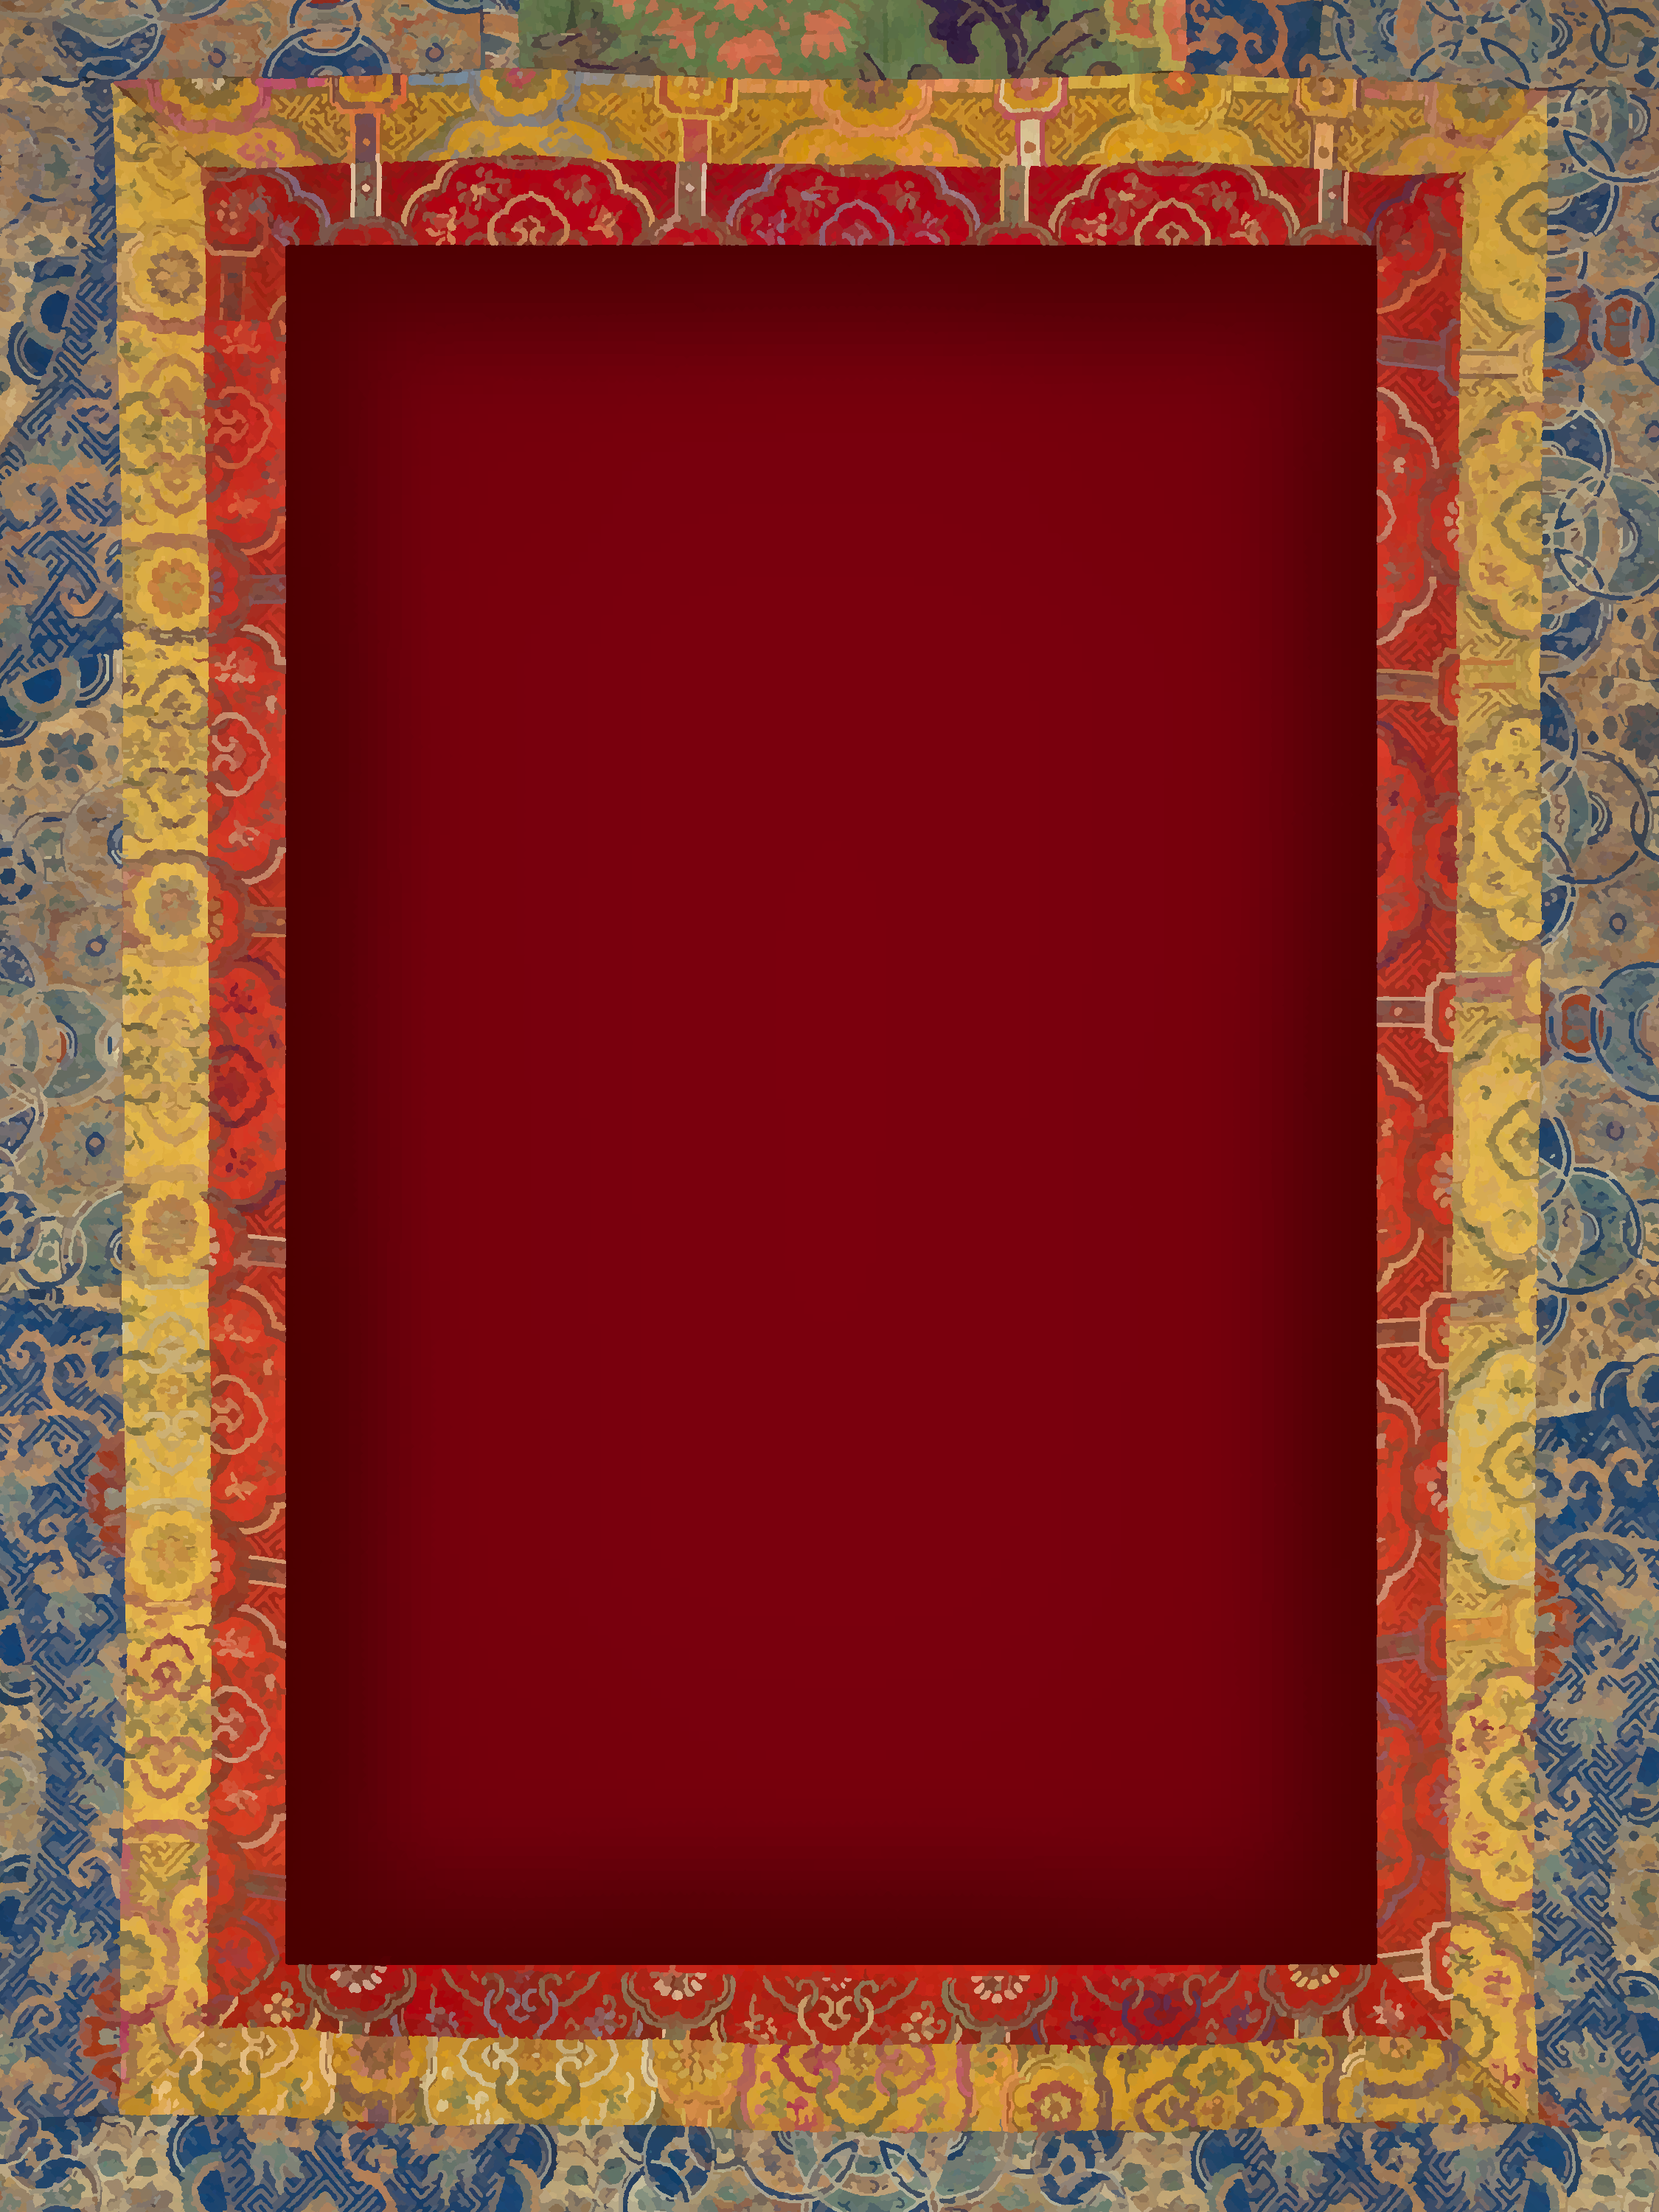
\includegraphics[width=\paperwidth,height=\paperheight]{tibet01.png}}

\let\oldquotation\quotation
\renewenvironment{quotation}
  {\par\noindent}
  {\par}
  
% fix toc page numbers
\let\origcftsecfont\cft
\let\origcftsecpagefont\cftsecpagefont
\let\origcftsecafterpnum\cftsecafterpnum
\renewcommand{\cftsecpagefont}{{\origcftsecpagefont}}
\renewcommand{\cftsecafterpnum}{{\origcftsecafterpnum}}
\let\origcftsubsecpagefont\cftsubsecpagefont
\let\origcftsubsecafterpnum\cftsubsecafterpnum
\renewcommand{\cftsubsecpagefont}{{\origcftsubsecpagefont}}
\renewcommand{\cftsubsecafterpnum}{{\origcftsubsecafterpnum}}
\let\origcftsubsubsecpagefont\cftsubsubsecpagefont
\let\origcftsubsubsecafterpnum\cftsubsubsecafterpnum
\renewcommand{\cftsubsubsecpagefont}{{\origcftsubsubsecpagefont}}
\renewcommand{\cftsubsubsecafterpnum}{{\origcftsubsubsecafterpnum}}

\renewcommand\thefootnote{{\bfseries\color{customColor}{\arabic{footnote}}}}
\let\oldfootnote\footnote
    \renewcommand{\footnote}[1]{\oldfootnote{{\bfseries\color{customColor}#1}}}
\begin{titlepage} % Suppresses headers and footers on the title page
	\centering % Centre everything on the title page
	%\scshape % Use small caps for all text on the title page

	%------------------------------------------------
	%	Title
	%------------------------------------------------
	
	\rule{\textwidth}{1.6pt}\vspace*{-\baselineskip}\vspace*{2pt} % Thick horizontal rule
	\rule{\textwidth}{0.4pt} % Thin horizontal rule
	
	\vspace{1\baselineskip} % Whitespace above the title

	{\scshape\Huge Matériaux pour servir\\ à l'Histoire de \\la Déesse Bouddhique \\T\={a}r\={a}}
	
	\vspace{1\baselineskip} % Whitespace above the title

	\rule{\textwidth}{0.4pt}\vspace*{-\baselineskip}\vspace{3.2pt} % Thin horizontal rule
	\rule{\textwidth}{1.6pt} % Thick horizontal rule
	
	\vspace{1\baselineskip} % Whitespace after the title block
	
	%------------------------------------------------
	%	Subtitle
	%------------------------------------------------
	
	{\scshape Par \\\Large Godefroy de Blonay} % Subtitle or further description
	
	\vspace*{1\baselineskip} % Whitespace under the subtitle
	
        {\scshape Élève diplômé de l'école pratique des hautes études} % Subtitle or further description
    
	%------------------------------------------------
	%	Editor(s)
	%------------------------------------------------
        \vspace*{\fill}

	\vspace{1\baselineskip}

	{\small\scshape Paris, 1895}
	
	{\small\scshape{Librairie Émile Bouillon, Éditeur\\67, Rue de Richelieu, au premier}}
	
	\vspace{0.5\baselineskip} % Whitespace after the title block

        \scshape Internet Archive Online Edition  % Publication year
	
	{\scshape\small Utilisation non commerciale --- Partage dans les mêmes conditions 4.0 International} % Publisher
\end{titlepage}
\setlength{\parskip}{1mm plus1mm minus1mm}
\clearpage
\tableofcontents
\clearpage
\section*{}
\paragraph{}
Le présent travail a pour sujet la déesse bouddhique T\={a}r\={a}. Jusqu'ici cette divinité n'était connue que par les rares mentions que lui accordaient les ouvrages généraux ; on savait aussi qu'un certain nombre d'hymnes adressés à cette divinité existaient en manuscrit dans les collections bouddhiques.

Je me suis proposé de coordonner les documents principaux que j'ai recueillis sur T\={a}r\={a}, afin qu'il fût possible de se rendre compte du rôle que cette divinité et son culte ont joue dans le bouddhisme.

Le hasard a mis à ma disposition trois textes qui caractérisent heureusement les différents aspects du sentiment religieux dans le bouddhisme :

Le \emph{Sragdhar\={a} stotra}, composé par Sarvaj\~{n}amitra, un lettré distingué qui se meut à l'aise dans les difficultés d'un mètre compliqué et qui met les ressources d'un style savant au service d'une foi ardente et d'une dévotion exaltée. Ce petit poème peut figurer parmi les inspirations les plus heureuses de la poésie personnelle à côté des \emph{Cent cinquante Stances de M\={a}t\d{r}ce\d{t}a}\footnote{Fujishima : \emph{Deux chapitres}, etc.} qu'I-Tsing admirait comme un chef-d'œuvre, et surpasse assurément en mérite littéraire les hymnes bouddhiques publiés jusqu'ici.\footnote{Minayeff : \emph{Mémoires de la Société Archéologique}, t. 2, fasc. 1, etc.}

Les \emph{Cent huit Noms de T\={a}r\={a}} ou \emph{\={A}ryat\={a}r\={a}n\={a}m\={a}\d{s}\d{t}ottara\'{s}atakastotra} forment avec l'œuvre de Sarvaj\~{n}amitra un étrange contraste. Pour parfaire le nombre consacré, qu'une superstition commune imposait aux bouddhistes aussi bien qu'aux brahmanes, l'auteur anonyme fait défiler une litanie d'épithètes incolores aisément transportables d'une divinité à l'autre, et qui n'ont d'autre vertu que de concourir au total obligatoire. La liste des \emph{Cent huit Noms} encadrée comme à l'ordinaire dans un dialogue, entre Vajrap\={a}\d{n}i et Avalokita, est sans nul doute un chapitre isolé d'un de ces tantras de T\={a}r\={a} auxquels Sarvaj\~{n}amitra fait allusion, où l'adoration de la déesse se mêlait à des pratiques magiques ou répugnantes.\footnote{Les catalogues nous font connaître les titres de plusieurs ouvrages qui se rattachent au culte tantrique de T\={a}r\={a} sans spécifier le caractère brahmanique ou bouddhique de la divinité : \emph{T\={a}r\={a}paddhati}, 170 p., 800 vers ; \emph{T\={a}r\={a}p\={u}janapaddhati}, 120 p., 1200 vers ; \emph{T\={a}r\={a}rahasyav\={a}rttika}, 250 p., 6000 vers ; \emph{T\={a}r\={a}bhaktisudh\={a}r\d{n}ava} ; \emph{T\={a}r\={a}nity\={a}rcanavidhi} (avec les mille noms de la déesse). Ces textes citent d'autres ouvrages intéressant T\={a}r\={a} : \emph{T\={a}r\={a}k\={a}ra\d{n}\={\i}ya}, \emph{T\={a}r\={a}r\d{n}ava}, \emph{T\={a}ropani\d{s}ad}. Voir : \emph{Pa\d{n}\d{d}it Dev\={\i}pras\={a}da}, Catalogue of the sansc. mss. existing in Oudh Province for the year 1889, 15. 21, 22, 23, et \emph{India Office, Cat. of sansc. mss.}, n° 2596 et 2603).}

L'\emph{Ekavi\d{m}\'{s}atistotra} est encore un fragment tantrique où les formules d'adoration se suivent à l'aventure sans que l'auteur ait pris même la peine de leur donner un cadre. La langue, la métrique et la raison sont violées avec un égale indifférence.

Mon travail eût été incomplet si je n'avait pas recherché les traces de T\={a}r\={a} dans les pays étrangers à l'Inde, où le bouddhisme a trouvé une grande faveur. Dans la littérature chinoise, je puis signaler plusieurs passages relatifs à T\={a}r\={a}, et je tiens à remercier M. Specht de l'obligeance avec laquelle il m'a prêté son précieux concours en ce domaine.

Le Tripi\d{t}aka chinois donne les titres des hymnes sanscrits que je publie ; le contenu que j'ai dû me contenter d'étudier sommairement semble répondre en partie seulement à mes textes.

Au Tibet, T\={a}r\={a} semble avoir été spécialement en honneur. Le bouddhisme a eu pour propagateur dans cette région le roi Srong-Tsan-Gampo. Les deux reines ses épouses le secondèrent de leur zèle et restèrent si populaires que la légende en fit les T\={a}r\={a}s tibétaines.

Au 16\textsuperscript{e} siècle encore, T\={a}ran\={a}tha, l'historien du bouddhisme indien, consacre une partie de son ouvrage à la biographie de saints personnages voués au culte de T\={a}r\={a}.

Ces biographies ne valent pas seulement par l'intérêt du conte, mais elles représentent certainement une tradition ancienne fondée sur des documents indiens. L'introduction de Jinarak\d{s}ita à son commentaire du \emph{Sragdhar\={a} stotra} montre que les légendes recueillies par T\={a}ran\={a}tha étaient déjà constituées définitivement dans l'Inde longtemps avant la compilation de l'auteur tibétain.

Qu'il me soit permis de remercier mon maître, M. Sylvain Lévi, des conseils et de l'aide patiente dont il n'a cessé de favoriser mes recherches. Si, grâce à lui, mon travail a quelque mérite, c'est pour moi un devoir et un privilège que de lui témoigner ici ma profonde gratitude.

\bigskip

G. B.
\clearpage
\section*{Bibliographie}
\begin{center}
\textbf{Ouvrages cités.}
\end{center}
\footnotesize
\paragraph{}
Aufrecht. --- \emph{Catalogus Codicum sanscritorum bibliothecæ bodleianæ.} Oxonii, 1864.

Balfour, Sr. G. Edw. --- \emph{The Cyclopedia of India and of Eastern and Southern Asia.}

Barth. --- \emph{Les religions de l'Inde.} Paris, 1876. Sandoz et Fischbacher.

Barth. --- \emph{Bulletin des religions de l'Inde}, dans \emph{Revue de l'histoire des religions.} 1889.

Bendall, Cecil. --- \emph{A Journey of literacy and archæological researches in Nepal and Northern India.} Cambridge, 1886.

Bendall, Cecil. --- \emph{Catalogue of buddhist-sanscrit manuscripts in the university library of Cambridge.} Cambridge, 1886.

Bhagvanlal Indraji. --- \emph{Inscriptions from Nepal} (\emph{Indian Antiq.}, vol. 9).

Bühler. --- Voir \emph{Indian Antiquary}, v. 2, p. 106.

Burgess. --- \emph{Elura Cave temples, Archæological Survey of Western India.} 1883.

Burgess, voir Fergusson.

Burnouf. --- \emph{Introduction à l'Histoire du Bouddhisme indien.} Paris, 1844.

\emph{Catalogue of the sansc. Mss.}, in the library of the India Office Part. 4, by Windisch and Eggeling. London, 1894.

Cunningham. --- \emph{Ancient Geography of India.} London, 1871.

Cowell et Eggeling. --- \emph{Catalogue of buddhist-sanscrit manuscripts in the possession of the Royal Asiatic Society} (Hodgson Collection). \emph{Journ. of R. A. S.}, new series, t. 8.

Csoma de Körös. \emph{Analyse du Kandjour}, trad., L. Feer. \emph{Annales du Musée Guimet.} T. 2.

Dowson, J. --- \emph{A classical Dictionary of Hindu mythology and history.} 1875. Trubner's Oriental Series.

Edkins. --- \emph{Chinese Buddhism.} London, 1880.

Eitel, Ernest. --- \emph{Handbook of Chinese buddhism.} London, 1888.

Fergusson et Burgess. --- \emph{The Cave Temples of India}, London, 1880.

Fleet. --- \emph{Corpus Inscriptionum Indicarum.} Calcutta, 1888.

Fleet. --- V. \emph{Indian Antiquary}, vol. 10. Bombay, 1881.

Fujishima, Ryauon. --- \emph{Deux chapitres extraits des Mémoires d'I-Tsing sur son voyage dans l'Inde, J. A.}, 1888.

Gaur Dás Bysack. --- \emph{Notice on a buddhist monastery at Bhot Bág\={a}n (Howrah), on two rare and valuable Tibetan mss.}, etc. \emph{J. of R. A. S.}, v. 59, 1890.

Hodgson, B. H. --- \emph{Essays on the language, litterature and religion of Nepal and Thibet.} London, 1874.

Hodgson. --- \emph{Quotations in Proof of his sketch of Buddhism. J. of R. A. S.}, old series, t. 2.

Hunter, W. --- \emph{Catalogue of the Hodgson's Manuscripts}, London, 1881.

Julien, Stanislas. --- \emph{Mémoires sur les contrées occidentales}, traduits du sanscrit en chinois en l'an 648 par Hiouen-Tsang et du chinois en français. Paris, 1858.

Kern. --- \emph{The Saddharma Pu\d{n}\d{d}ar\={\i}ka} (Sacred Books of the East, v. 21).

Kern. --- \emph{Der Buddhismus und seine Geschichte in Indien.} Trad. Jacobi, Leipzig, 1884.

Kielhorn. --- v. \emph{Ind. Ant.}, v. 17. \emph{A buddhist Stone Inscription from Sravasti.}

Klaproth, Julius. --- \emph{Reise in den Caucasus und nach Georgien.} Halle-Berlin, 1812.

Langlois, M.-A. --- \emph{Harivansa, ou histoire de la famille de Hari}, traduit sur l'original sanscrit. Paris, 1834.

Lavallée-Poussin, Louis de --- \emph{Bodhicary\={a}vat\={a}ra}, v. \emph{Muséon}, t. 11. Louvain, 1892.

Lévi, Sylvain. --- \emph{Le Théâtre indien.} Paris, 1890.

Minayeff. --- \emph{Recherches sur le Bouddhisme}, trad. Assier de Pompignan. Paris, 1894.

Mitra, R\={a}jendral\={a}la. --- \emph{The sanscrit buddhist Literature of Nepal.} Calcutta, 1882.

Mitra, R\={a}jendral\={a}la. --- \emph{Buddha Gaya, the hermitage of Sakyamuni.} Calcutta, 1878.

Oldenberg. --- \emph{Le Buddha}, trad. A. Foucher. Paris, 1894.

Pa\d{n}\d{d}ita Devi Prasáda. --- \emph{A Catalogue of sanscrit manuscripts existing in Oudh Province for the year 1889, compiled} Allahabad, 1893.

R\={a}jatarangin\={\i}. --- Voir Stein, et Troyer.

Schiefner, Anton. --- \emph{T\={a}ran\={a}thas Geschichte des Buddhismus in Indien}, aus dem Tibetischen übersetzt. Saint-Petersburg, 1869.

Schlagintweit, E. de --- \emph{Le Bouddhisme au Thibet.} Annales du Musée Guimet, t. 3.

Stein, M. A. --- \emph{Kalha\d{n}a's R\={a}jatara\.{n}gi\d{n}\={\i}, or Chronicle of the Kings of Kashmir.} Bombay, 1892.

Svayambhupur\={a}na. --- Manuscrit devanagari, n. 78, Cat. Bibl. Nat.

T\={a}ran\={a}tha. --- Voir Schiefner.

Troyer. --- \emph{R\={a}jatara\.{n}gi\d{n}\={\i}, histoire des rois du Kasmir}, trad. Paris, 1840.

Waddell. --- \emph{J. of R. A. S.}, janv. 1894.

Wassiliew, W. --- \emph{Der Buddhismus, seine Dogmen Geschichte und Litteratur.} Saint-Pétersbourg, 1860.

Wright. --- \emph{History of Nepal.} Cambridge, 1877.

Wilson, H. H. W. --- \emph{Works}, etc., London, 1861-1877.
\clearpage
\normalsize
\section{Sources Littéraires}
\paragraph{}
Les documents les plus complets que nous ayons sur le personnage et le culte de la déesse bouddhique T\={a}r\={a} appartiennent à la littérature sanscrite népalaise. Ce sont le \emph{Sragdhar\={a}stotra} avec son introduction dans la \d{t}\={\i}k\={a} de Jinarak\d{s}ita, la liste des \emph{Cent huit noms de T\={a}r\={a} : \={A}ryat\={a}r\={a}n\={a}m\={a}\d{s}\d{t}ottara\'{s}ataka}, et l'\emph{Hymne en vingt et un vers : Ekavi\d{m}\'{s}atistotra}.

Il a dû exister encore d'autres textes relatifs à T\={a}r\={a} qui seraient précieux à retrouver ; c'est à T\={a}ran\={a}tha que nous devons d'en connaître au moins deux par leurs titres ; il dit à propos de l'\={a}c\={a}rya R\={a}hulabhadra : « Son histoire est racontée dans la \emph{Description de la vie de T\={a}r\={a}.}\footnote{T\={a}ran\={a}tha, p. 93.} » Les informations de T\={a}ran\={a}tha ne déterminent malheureusement ni la date ni l'origine sanscrite ou tibétaine de cet écrit.

L'autre est le \emph{T\={a}r\={a}s\={a}dhana\'{s}ataka}, par Candragomin ; T\={a}ran\={a}tha nous apprend que cet ouvrage a été traduit en tibétain.\footnote{T\={a}r., p. 156.}

Le catalogue du Kandjour nous apprend l'existence dans le canon tibétain des textes suivants en rapport avec le culte de T\={a}r\={a} :
\begin{table}[H]
    \centering
    \bfseries
    \footnotesize
    \begin{tabular}{|l|l|p{28mm}|p{38mm}|}
    \hline
        Rgyud & 4 & 13 & T\={a}r\={a}kurukullakalpa. \\ \hline
        Rgyud & 14 & 49 & Sarva Tath\={a}gata m\={a}t\={a}n\={\i} T\={a}r\={a} vi\'{s}vakarma bhava tantra. \\ \hline
        Rgyud & 14 & 50 & \={A}rya T\={a}r\={a} bhadra n\={a}ma a\d{s}\d{t}a\'{s}atakam. \\ \hline 
        Rgyud & 14 & 51 & T\={a}r\={a} Dev\={\i} n\={a}m\={a} a\d{s}\d{t}a\'{s}atakam. \\ \hline
        Rgyud & 14 & 53 & T\={a}r\={a} svapratij\~{n}\={a} dh\={a}ra\d{n}\={\i} (mantra). \\ \hline 
        Rgyud & 18 & Bhagavaty \={A}rya T\={a}r\={a} m\={u}lakalpa. & ~ \\ \hline
        Rgyud & 21 & 3 & Origine des noms des divinités, parmi lesquelles T\={a}r\={a}. \\ \hline
    \end{tabular}
\end{table}
\paragraph{}
On trouve dans le Tandjour, Rgyud 1, 9 un T\={a}r\={a}mah\={a}yogatantra.

La source la plus féconde en renseignements sur le grand développement que prit le culte de T\={a}r\={a} est l'\emph{Histoire du Bouddhisme aux Indes} de T\={a}ran\={a}tha. Le culte de cette divinité devait avoir conservé une importance particulière pour que l'auteur de l'\emph{Histoire du Bouddhisme} nous rapporte une quantité relativement considérable de renseignements au sujet de T\={a}r\={a} ; elle avait parmi les plus notables \={a}c\={a}ryas de l'Inde des sectateurs fervents.

La popularité de T\={a}r\={a} au Tibet se constate dès une époque assez ancienne : Les Tibétains ont identifié T\={a}r\={a} avec les deux femmes du roi Srong-Tsan-Gampo, l'introducteur du bouddhisme en ce pays (septième siècle \textsc{ce}).\footnote{Voir Schlagintweit. \emph{Bouddhisme au Tibet}, 40-42, Waddel, \emph{J. R. A. S.}, janvier 1894.} Les deux épouses royales étaient, en tibétain : Dolkar (pron. Dö-Kar') et Dol-jang (pron. Dö-jang ou Dö-ngön), la T\={a}r\={a} blanche et la T\={a}r\={a} verte. Elles portent aussi l'une et l'autre le nom de S'grolma (pron. 'Döma'). L'une était princesse népalaise,\footnote{Nommée Vajrabhr\={u}ku\d{t}i ou Bribsun fille du roi Prabh\={a}varman ou A\d{m}\'{s}uvarman, 630-640 \textsc{ce}.} l'autre princesse chinoise\footnote{Fille de l'empereur Tai-Tsung, elle épousa le roi en 630 \textsc{ce}. V. Gaur Dàs Bysack. \emph{J. A. S.}, vol. 59, p. 53.} ; ces deux princesses personnifient donc deux influences bouddhiques aussi intenses l'une que l'autre.

L'histoire de la T\={a}r\={a} tibétaine, ou des T\={a}r\={a}s tibétaines, car leur nombre finit par devenir considérable, échappe à nos moyens actuels d'investigation ; il faudrait entreprendre l'examen de documents littéraires bien peu accessibles encore. Klaproth\footnote{\emph{Reise in den Caucasus und nach Georgien}, v. 1, p. 213-215.} donne en allemand un hymne à la verte Darra\d{h} ou Rogon-Darrki, hymne peu caractéristique. M. Waddell\footnote{\emph{J. R. A. S.}, janvier 1894.} a étudié ce sujet spécialement et a publié la traduction anglaise d'hymnes extraits du manuel d'adoration à T\={a}r\={a}, hymnes assez semblables à ceux que nous traduisons. Il y a joint la liste d'un certain nombre de T\={a}r\={a}s, sans donner malheureusement ses sources.

La Chine fournit aussi à nos recherches son contingent de renseignements et de documents.

Hiouen-Tsang mentionne T\={a}r\={a} à deux reprises :
\begin{quotation}
« Au couvent\footnote{St. Julien, v. 2, p. 439-440.} Til\={a}\d{d}haka (dans le Magadha), dans le vih\={a}ra du milieu, il y a une statue droite du Buddha haute de trente pieds. A gauche s'élève la statue de To-lo-pou-sa (T\={a}r\={a}bodhisattva) et à droite celle de Kouan-tseu-thsaï-pou-sa (Avalokite\'{s}varabodhisattva). Ces trois statues sont en laiton fondu, leur aspect divin inspire une crainte respectueuse et les effets de leur puissance se répandent secrètement au loin.\footnote{C'est à M. Specht que je dois la connaissance de ces deux passages avec leur portée précise, qui a échappé à Stanislas Julien.} »
\end{quotation}
\paragraph{}
Puis dans la description du royaume de Vai\'{s}\={a}l\={\i}\footnote{St. Julien, v. 3, p. 40 et suiv.} :
\begin{quotation}
« A deux ou trois lis au nord de la statue en cuivre du Buddha exécutée par le roi Mouan-Tscheou (Po\={u}r\d{n}avarma) on voit au milieu d'un vih\={a}ra en briques la statue de To-lo-pou-sa (T\={a}r\={a}bodhisattva). Elle est d'une grande hauteur et douée de pénétration divine. Le premier jour de chaque année on lui fait de riches offrandes. Les rois, les ministres et les hommes puissants des royaumes voisins présentent des fleurs d'un parfum exquis en tenant des étendards et des parasols ornés de pierres précieuses. Les instruments de métal et de pierre résonnent tour à tour, les guitares et les flûtes unissent leurs sons harmonieux. Ces assemblées religieuses durent pendant sept jours.\footnote{St. Julien, v. 3, p. 50-51.} »
\end{quotation}
\paragraph{}
Il est fait mention aussi de T\={a}r\={a} dans le livre : \emph{Les pays du Buddha}, chapitre 4, description de toute l'Inde et route pour y aller. L'auteur Tao-Suen, le fondateur de l'École du Vinaya en Chine (650 \textsc{ce}) mentionne dans le royaume de Tsauk\={u}\d{t}a près du Str\={\i}r\={a}jya, par conséquent dans l'Asie centrale, un st\={u}pa de T\={a}r\={a}.

Grâce à l'obligeance de M. Édouard Specht qui m'en a signalé l'existence, je puis constater la présence dans le \emph{Tripi\d{t}aka} chinois de deux textes relatifs à T\={a}r\={a} :

Le premier donne une transcription en caractères chinois d'un texte sanscrit : \emph{Les cent huit noms de la Sainte T\={a}r\={a}}.

Quoique ce titre nous permît d'espérer trouver la transcription du texte que nous donnons plus loin en sanscrit, il a fallu renoncer à cette identification, car nous nous trouvons en présence de dh\={a}ra\d{n}\={\i}s sans caractère propre. Le texte commence ainsi :

Ôm, trailokye, vijaye, artha\d{m}jaye, ari\d{m}ghate, jaye, ajaye, vijaye, mah\={a}jaye, vijaye, jaye, jaye, hi hi ... etc.\footnote{Voir \emph{Ta Ts'ang King}, boîte 27, cahier 11, de l'exemplaire de la Société asiatique.}

Les qualificatifs sont donnés en transcription et le texte sous forme de s\={u}tra est donné en traduction chinoise. Le bodhisattva Avalokita est un des interlocuteurs, comme dans le texte sanscrit.

Le second texte donne aussi une transcription en caractères chinois d'un texte sanscrit, ayant pour titre : Chan-to-lo-pou-sa-fan-tsan équivalant au sanscrit : \={A}rya t\={a}r\={a} bodhisattva sa\d{m}sk\d{r}ta stotra, soit : \emph{Éloge en sanscrit de la sainte T\={a}r\={a} bodhisattva}.\footnote{\emph{Ta Ts'ang King}, b. 27, c. 13.}

Le nombre des indications fournies par le bouddhisme chinois donne le droit de penser que le bouddhisme japonais a conservé aussi un souvenir plus ou moins vivace de T\={a}r\={a}. Malgré les efforts que nous avons tentés dans cette direction, à cause peut-être de l'insuffisance des moyens d'investigation dont nous disposions, il ne nous a pas été donné de suivre T\={a}r\={a} jusqu'au Japon.

M. Horiu Toki, d'après des notes prises dans les documents japonais du Musée Guimet, a pu nous signaler le nom de \={A}rya T\={a}r\={a} bodhisattva passé au Japon, sous la forme de Ro-tara-ni-bi. « Elle est comme le bateau qui fait traverser à l'homme l'Océan, et lui procure la liberté (d'après le Yoga-ki). »

Le bouddhisme du sud n'accorde point de place aux énergies féminines des Buddhas (\emph{\'{s}aktis}), aussi T\={a}r\={a} est-elle restée étrangère à la littérature sacrée de Ceylan.\footnote{Barth. \emph{Bulletin des religions de l'Inde}, 1889, 2 part. p. 5.}
\clearpage
\section{Documents Épigraphiques}
\paragraph{}
Les documents épigraphiques seraient les fondements historiques les plus sûrs pour assigner des dates précises aux phases du culte de T\={a}r\={a} aux Indes. D'après les légendes il y a eu une quantité de temples et de collèges consacrés à ce culte. T\={a}ran\={a}tha mentionne des fondations de ce genre extrêmement nombreuses. Un examen détaillé des ruines bouddhiques de l'Inde permettra peut-être de trouver plus de vestiges que nous n'avons pu le faire en nous aidant de ce qui a été publié jusqu'à présent.

Un document précieux, le plus ancien en date, se trouve dans l'île de Java. M. Brandes l'a publié tout au long, texte et traduction, sous le titre : \emph{Een n\={a}gar\={\i} opschrift gevonden tusschen Kalasan en Prambanan}.\footnote{Voir : \emph{Tijdschrift von indische Taal-Land-en-Volkerkunde.} (Batavia, 1886.)}

Le texte mutilé au début est de douze strophes en vers, soit vasantatilaka, soit \={a}ry\={a} ; je donne ici la traduction complète du texte, plus le texte de l'invocation initiale à T\={a}r\={a} :
\begin{quotation}
« Hommage à la bienheureuse \={A}rya T\={a}r\={a}. »

\bigskip

« 1. Elle qui délivre directement de cet état infini de malheur ... ce qui concerne la nature de ce qui est terrestre et de ce qui est invisible ... l'essence du salut du monde inférieur, des dieux et des hommes ... seule T\={a}r\={a}. »

« Namo bhagavaty\={a}y \={a}ryat\={a}r\={a}yai \texthindi{॥} y\={a} t\={a}rayaty amitadu\d{h}khabhav\={a}t tiryag na \texthindi{।} lokavilokyavidhiva ... rup\={a}ya\d{h} \texthindi{॥} s\={a}ra\d{h} surendran\={a}ralokavibh\={u}tis\={a}ra\d{m} \texthindi{।} t\={a}r\={a}di ... bhimata\d{m} jagad ekat\={a}r\={a}. »

\bigskip

« 2. Car les gurus du prince \'{S}ailendra ont fait construire un temple majestueux à T\={a}r\={a}. 3. Sur l'ordre des gurus une déesse a été fabriquée par les reconnaissants, et aussi un temple pour elle et aussi un lieu de séjour pour les nobles moines qui connaissent le Mah\={a}y\={a}na de la doctrine du Vinaya. 4. Sous la surveillance des \={A}de\'{s}a\'{s}\={a}strin du prince, nommés le Pa\~{n}kura, le Taw\={a}na, le T\={\i}ripa,\footnote{Fonctionnaires dont on ignore le rôle précis.} a été construit ce temple de T\={a}r\={a} et aussi un lieu de séjour pour les nobles moines 5. dans le royaume florissant du prince qui est l'ornement de la dynastie des \'{S}ailendras, (d'après les désirs) des gurus de ce prince des \'{S}ailendras auxquels il est satisfait de cette façon : un temple à T\={a}r\={a} a été élevé 6. après que sept siècles se sont écoulés dans l'ère du prince des \'{S}akas ; le prince, pour honorer ses gurus, à la suite d'un vœu, a construit un temple à T\={a}r\={a}. 7. Le domaine du village, nommé K\={a}lasa, est donné à l'assemblée en présence du Pa\~{n}kura, du Taw\={a}na, du T\={\i}ripa et des notables chefs du village. 8. Ce don, à la façon bhura, donné à l'église par le prince, ne peut pas être aboli par les princes de la race \'{S}ailendra, mais doit être indéfiniment respecté 9. aussi par les Pa\~{n}kura, les Taw\={a}nas, et les T\={\i}ripas et leurs respectables femmes 10. et le roi demande aussi à tous les princes qui régneront plus tard, ceci, qu'il exige : « Puisse cette digue du droit qui est commun à tous, de tout temps être protégée par vous. » 11. Puissent en suite de cette sainte fondation tous les gens avoir connaissance des vibh\={a}gas et des prescriptions du Tribhav\={a} (?). 12. Sa majesté fait un vœu kariy\={a}na, elle prie les princes qui régneront ici plus tard de protéger de plus en plus cette fondation, toujours. »
\end{quotation}
\paragraph{}
Dans cette inscription, rien qui soit très personnel à T\={a}r\={a} et qui se rapproche de nos hymnes, d'autant plus que la première strophe est particulièrement mutilée. Néanmoins, il est important à constater que T\={a}r\={a} a pénétré en même temps que le bouddhisme à Java où son culte, comme partout ailleurs, est attaché à la tradition du Mah\={a}y\={a}na.

La date de l'inscription, donnée dans l'ère \'{S}aka, correspond à 779 \textsc{ce} (un siècle après Sarvaj\~{n}amitra).

Un des documents les plus importants a été publié par M. Fleet\footnote{\emph{Indian Antiquary}, v. 10, p. 185. Je cite presque textuellement cet article.} ; Elliot en avait donné une transcription.\footnote{Elliot, \emph{Mss. collection}, vol. 1, p. 356.} C'est une inscription trouvée sur une tablette de pierre, près d'un temple jaina, dans le fort de Dan\d{m}bal. Les emblèmes figurés sur la pierre sont décrits au chapitre suivant.\footnote{V. \emph{inf.}, p. 9.} Le texte est édité d'après un estampage de M. H. Cousens. Le texte est en écriture vieux canarais, délicatement gravé et parfaitement conservé. Autour du sommet de la tablette deux longues lignes de même écriture contiennent trois vers sanscrits. L'inscription est du temps du roi C\={a}lukya Tribhuvanamalla ou Vikram\={a}ditya 6, elle est datée du Juva sa\d{m}vatsara, la dix-neuvième année du C\={a}lukya-Vikramavar\d{s}a, ère qui fut fondée par ce prince et qui part de son avènement en l'année \'{s}aka 1017, soit 1095-6 \textsc{ce}. L'inscription donne le nom de la reine Lak\d{s}m\={a}dev\={\i}, qui gouvernait la région nommée « les dix-huit agrah\={a}ras » et la ville de Dharmapura ou Dharmavolal, la ville de la religion, qui est certainement Da\d{m}bal même. Il y avait alors à Da\d{m}bal un vih\={a}ra bouddhique construit par les seize se\d{t}\d{t}his (\'{S}re\d{s}\d{t}hin, marchands) de l'endroit, et un vih\={a}ra de T\={a}r\={a}dev\={\i} construit par le se\d{t}\d{t}hi Sa\d{m}gavaya de Lokkigu\d{n}\d{d}i, tandis que cette ville était jaina et que ces marchands appartenaient à la secte V\={\i}rabala\~{n}ja, qui plus tard adopta le culte lingaïte de Basava\footnote{Voir Wilson, \emph{Religious sects of the Hindus}, p. 225 sqq.} : une preuve de plus de la profonde influence que tous ces cultes hindous parallèles exerçaient les uns sur les autres.

Voici les passages de l'inscription qui sont spécialement relatifs à T\={a}r\={a}.
\begin{quotation}
l. 1. « Hommage à Buddha, hommage à toi, ô sainte T\={a}r\={a}, qui apaises la crainte des lions, des éléphants, du feu, des serpents à chaperon, des voleurs, des chaînes, de l'eau, de l'océan. --- Toi qui es revêtue d'une splendeur semblable à celle des rayons de la lune. Qu'elle donne toujours sa bénédiction, cette T\={a}r\={a} qui apaise la misère de l'affliction de l'existence, qui sortit du barattement de l'océan du savoir nommé Praj\~{n}\={a} ; elle qui donne la puissance au Buddha, qui est l'incarnation suprême de la parfaite sagesse dans les trois mondes, qui demeure dans le cœur du Tath\={a}gata de même que le disque de la pleine lune dans le ciel. »

\bigskip

l. 19. « Hommage à la déesses, la sainte T\={a}r\={a}dev\={\i} et au dieu Buddha. (Qu'on donne) un mattar de terrain de jardin en concession, à la façon sarvanamasya, dans le domaine Ponnakuruva, à l'est du village, et un aruvana et trois gadyanas d'or à percevoir chaque année comme taxe, dont on profitera avec jouissance pour l'entretien convenable du culte, pour l'approvisionnement de parfums, fleurs, encens, lampes et guirlandes, et pour l'offrande perpétuelle et autres choses, --- pour l'entretien du p\={u}j\={a}ri, pour fournir de nourriture et de vêtements les religieux mendiants du lieu, et pour subvenir aux frais de restauration. »
\end{quotation}
\paragraph{}
Voici la traduction des trois lignes sanscrites qui encadrent l'image :
\begin{quotation}
« ... T\={a}r\={a} puisse-t-elle, elle qui se préoccupe avec anxiété de témoigner sa tendresse, préserver les hommes que tourmente la crainte de l'eau, des rois, des masses, du feu, du vent, elle qui ôte la crainte des audacieux, des océans, des éléphants, des lions ... qui accorde sans délai les récompenses désirées ! Que Sa\d{m}gama nous préserve toujours ! »
\end{quotation}
\paragraph{}
L'épigraphie de T\={a}r\={a} est étroitement apparentée à sa littérature ; elle est dans l'une et dans l'autre la sauveuse par excellence, celle qui prend soin d'écarter de ses adeptes les craintes et les supplices ; elle occupe une place prépondérante à côté du Buddha qui lui doit sa sagesse, et dont elle est le principal ornement. Les vers sanscrits de l'inscription sont presque des citations de nos stotras, ou du moins ils les reflètent indirectement par l'intermédiaire d'une tradition précise et fidèle.

Une inscription bouddhique de \'{S}r\={a}vast\={\i} (Oudh), plus récente encore que celle de Da\d{m}bal puisqu'elle date de l'an 1219 \textsc{ce}, contient une mention de T\={a}r\={a} qui suffit à prouver la persistance vivace de son culte.\footnote{\emph{Indian Antiquary}, vol. 17, p. 62.}

La déesse est adorée en ces termes :
\begin{quotation}
l. 2. Sa\d{m}s\={a}r\={a}mbhodhit\={a}r\={a}ya t\={a}r\={a}m utt\={a}ralocan\={a}m \texthindi{।} vande g\={\i}rvv\={a}\d{n}av\={a}\d{n}\={\i}n\={a}\d{m} Bh\={a}rat\={\i}m adhidevat\={a}m. \texthindi{॥}

\bigskip

« Pour traverser l'océan des existences, j'adore la sauveuse Bh\={a}rat\={\i}, T\={a}r\={a}, qui a des yeux dont saillent les pupilles, la déesse souveraine des paroles des dieux. »
\end{quotation}
\paragraph{}
T\={a}r\={a} est encore celle qui fait traverser et son nom conserve ici toute sa puissance étymologique.
\clearpage
\section{Les Images de T\={a}r\={a}}
\paragraph{}
Les images de T\={a}r\={a}, identifiées jusqu'ici, sont peu nombreuses. Une enquête diligente permettra sans aucun doute d'en reconnaître bien davantage, même dans les monuments déjà explorés, et particulièrement (au témoignage de M. Waddell) dans le pays de Magadha.

Près d'un temple Jaina, dans le fort de Da\d{m}bal,\footnote{V. Fleet. \emph{Indian Antiquary}, v. 10, p. 185.} sur une tablette de pierre, outre l'inscription mentionnée plus haut se trouve une figure représentant T\={a}r\={a}, assise à l'intérieur d'une châsse, regardant devant elle, tenant dans sa main gauche un nymphéa épanoui et dans sa main droite un objet difficile à identifier. A la droite de la divinité, une vache et un veau ; le soleil au-dessus d'eux ; à gauche, une figure debout, les mains jointes sur le visage, en adoration, un nénuphar à huit pétales sur les mains, deux candélabres à mèches allumées derrière elle, et la lune au-dessus. L'image, en somme, ne présente pas de traits caractéristiques.

A Buddha Gay\={a},\footnote{\emph{Buddha Gay\={a}}, par R\={a}jendral\={a}la Mitra. 1878, pl. 20, fig. 1.} sur l'emplacement d'un temple voué à T\={a}r\={a}, on a trouvé une figure sculptée que R\={a}jendral\={a}la Mitra dit être Padmap\={a}\d{n}i, et qui ensuite passa pour une T\={a}r\={a}, lorsque le temple fut consacré au culte de cette divinité. Buchanan Hamilton\footnote{Même ouvrage, p. 60.} est d'accord pour constater que ce n'est pas du tout une image originale de T\={a}r\={a}, mais un personnage masculin.

A Ellora, Burgess\footnote{Burgess. \emph{Ellora Cave Temples}, cave 12.} a constaté la présence d'une statue de T\={a}r\={a}, avec un lotus, au-dessous d'une niche.

T\={a}ran\={a}tha\footnote{T\={a}r., p. 160.} parle d'une statue d'elle, élevée par Vin\={\i}tasena dans un temple, qui fut transportée à Devagiri par crainte des dégâts que commettaient les Turu\d{s}kas.

Il semble que les diverses T\={a}r\={a}s se distinguaient par la couleur. Chacune d'elles portait les couleurs de son Buddha respectif.\footnote{Voir Wright, \emph{History of Nepal}, plate 5, p. 28. Kern, \emph{Buddhismus}, vol. 2, p. 215-16. Hodgson, \emph{J. R. A. S.}, old s., v. 2, p. 319 et suiv.}

\begin{table}[H]
    \centering
    \bfseries
    \begin{tabular}{|l|l|l|}
    \hline
        \textbf{Buddha:} & \textbf{T\={a}r\={a}:} & \textbf{Couleur:} \\ \hline
        Ak\d{s}obhya & Locan\={a} & bleu \\ \hline
        Ratnasa\d{m}bhava & M\={a}mak\={\i} ou M\={a}muk\={\i} & jaune ou or \\ \hline
        Vairocana & Vajradh\={a}tv\={\i}\'{s}var\={\i} & blanc \\ \hline
        Amit\={a}bha & P\={a}\d{n}\d{d}ar\={a} ou P\={a}\d{n}\d{d}ur\={a} & rose, rouge \\ \hline
        Amoghasiddha & T\={a}r\={a}\tablefootnote{Voir le manuscrit add. 1476 (Dh\={a}ra\d{n}\={\i}s) du catalogue de Cecil Bendall, qui contient p. 22 b. une T\={a}r\={a} dont la tête et les membres sont verts. Cette miniature fort belle est du 17\textsuperscript{e} siècle.} & vert \\ \hline
    \end{tabular}
\end{table}
\paragraph{}
La position des mains varie aussi de l'une à l'autre.

Le Népal, le Tibet et la Mongolie sont d'accord sur la répartition de ces couleurs, c'est surtout dans ces pays que les images des Dhy\={a}nibuddhas et de leurs T\={a}r\={a}s ont été les plus nombreuses et les plus spécialement révérées.

Au Tibet,\footnote{Schlagintweit. \emph{Le Bouddhisme au Thibet}, p. 42.} comme nous l'avons vu, on connaît deux T\={a}r\={a}s : Dolkar et Doljang. On les représente toutes deux dans la même attitude ; le pied droit pendant devant le trône, la main droite tenant le lotus bleu. Leur teint est différent : Dolkar est blanche, Doljang est verte. Elles sont censées créées par le rayon bleu qui sortait de l'œil gauche d'Amit\={a}bha s'incarnant en elles.\footnote{Schlagintweit, p. 54.} Certaines représentations de Doljang montrent cet œil de sagesse dessiné dans la paume de ses mains et sous la plante de ses pieds ; ces marques ont même une ressemblance surprenante avec les stigmates chrétiens.\footnote{Schlagintweit, p. 138.} Le Musée Guimet\footnote{Salle 2, vitrine 13, partie verticale, second rang (catal. p. 55).} possède une statuette de bronze représentant Doljang ou Dolkar assise sur un lotus, la jambe droite pendante, coiffée d'une couronne.

La T\={a}r\={a} japonaise tiendrait de très près à la T\={a}r\={a} tibétaine d'après le témoignage de M. Horiu Toki, fondée sur le Yoga-ghi-Ki. Elle serait verte mêlée de blanc, née des yeux de Kouan-in, elle se nomme aussi Fou-ghen, et fait partie du groupe de Kouan-in.

En somme, à en juger sur ces indications trop rares, rien n'a distingué T\={a}r\={a}, au point de vue artistique, de bien d'autres figures féminines que l'art hindou a produites ; de même que la littérature l'a habillée non seulement de toutes les épithètes bouddhiques en vogue, mais encore des qualités et attributs chers au panthéon brahmanique, de même il est difficile de croire qu'une forme extérieure bien arrêtée ait jamais été consacrée à T\={a}r\={a}.

Dans le \emph{Sragdhar\={a} Stotra}, quoiqu'au point de vue de la charité T\={a}r\={a} ne varie jamais, son apparence néanmoins revêt les aspects les plus divers ; on la voit les pieds illuminés de l'éblouissement de ceux qui l'adorent,\footnote{\emph{Srag.}, vers 1.} dorée comme le soleil levant,\footnote{\emph{Srag.}, v. 5.} courbant sous son poids les têtes d'Indra, Rudra et Brahm\={a}, se tenir dans l'attitude de l'\={a}l\={\i}\d{d}ha qui est une de celles du tireur d'arc, la jambe droite en avant, la gauche repliée\footnote{\emph{Srag.}, v. 30.} ; ou bien, emportée de colère\footnote{\emph{Srag.}, v. 31.} elle est revêtue d'armes étincelantes et des serpents affreux lui enserrent les bras, analogue à K\={a}l\={\i}\footnote{Comp. Buchanan Hamilton. \emph{Tantra S\={a}ra. Transact. R. As. S.}, 1, 45.} ; ou bien, plus calme,\footnote{\emph{Srag.}, v. 32.} tous les personnages célestes et terrestres lui offrent leurs hommages et, conclut Sarvaj\~{n}amitra, « la déesse pareille au cristal qui reflète tout ce qui l'entoure, à sa fantaisie se pare de la pourpre du soleil levant, plus rouge que la laque, d'une couleur sombre plus sombre que le saphir ou la feuille écrasée du lotus, d'un blanc plus blanc que le lait baratté de l'océan.\footnote{\emph{Srag.}, v. 33.} »

Cette énumération de couleurs, d'accord avec les couleurs des Buddhas et des T\={a}r\={a}s données plus haut pourrait n'être pas fantaisiste et tenir de la tradition ; le bleu, le blanc, le rouge y sont, manqueraient le jaune et le vert pour que la concordance fût complète, et encore le vert on le trouve à côté du bleu-saphir dans la poussière de la feuille du lotus, et l'or ou jaune est tout naturellement impliqué dans la comparaison avec le soleil.

Dans la liste des \emph{Cent huit noms d'\={A}rya T\={a}r\={a}} comme dans toutes les énumérations de ce genre, T\={a}r\={a}\footnote{\emph{108 noms}, v. 26.} a mille bras, mille yeux, elle a le visage sombre et revêt toutes les formes.\footnote{\emph{108 noms}, v. 28.} Avec l'éclat du feu, elle a de grands yeux,\footnote{\emph{108 noms}, v. 34.} porte toutes les armes, s'orne de crânes\footnote{\emph{108 noms}, v. 37.} ... etc.

Évidemment, ce qui ressort le plus clairement de nos hymnes, c'est le privilège qu'a T\={a}r\={a} de revêtir à son gré la forme extérieure qui lui convient, et n'est-ce pas là le privilège indispensable au rôle de charité universelle qu'elle joue\footnote{Voir : \emph{Naip\={a}l\={\i}yadevat\={a}kaly\={a}\d{n}apa\~{n}cavi\d{m}\'{s}atik\={a}}, v. 1 (Wilson, Works, vol. 2).} ? Elle est la \emph{très bonne}. Elle paraît à l'up\={a}saka \'{S}\={a}ntivarman sous la forme d'une vieille femme pour lui faire traverser un fleuve\footnote{T\={a}r., p. 142.} : elle se dépouille de ses joyaux en faveur d'une pauvre vieille lorsque Candragomin\footnote{T\={a}r., p. 157.} adresse une prière à l'image qui la représente et depuis lors la peinture resta sans bijoux.
\clearpage
\section{Le Rôle de T\={a}r\={a} dans T\={a}ran\={a}tha}
\paragraph{}
T\={a}ran\={a}tha, nous l'avons dit, nous fournit dans son \emph{Histoire du Bouddhisme}, les noms et l'histoire d'une série de fidèles de T\={a}r\={a}. Il faut les reprendre un à un pour suivre, d'après un ordre aussi chronologique que possible, le développement de ce culte au travers des cinquième, sixième, septième et huitième siècles de notre ère.

Le premier personnage en date qui soit mentionné est l'\={a}c\={a}rya K\={a}la\footnote{T\={a}r., p. 89.} dont la personnalité est bien difficile à identifier au milieu du grand nombre de noms qui lui sont donnés\footnote{T\={a}r., p. 90 et Kern. \emph{Buddhismus}, 7, 464.} : K\={a}la, M\={a}t\d{r}ce\d{t}a,\footnote{I-Tsing nous donne la transcription chinoise de ce nom : Mot'ch'a-li-tchi-tch'a dans le chap. 35 de l'\emph{Histoire de la loi intérieure envoyée de la mer du Sud}. Voir Ryauon Fujishima. \emph{J. As.}, 1889, 2 chap. d'I-Tsing.} Pit\d{r}ce\d{t}a, A\'{s}vagho\d{s}a, Durdhar\d{s}a, Durdhar\d{s}ak\={a}la, Dh\={a}rmika, Subh\={u}ti, Maticitra, \'{S}\={u}ra.

T\={a}ran\={a}tha place la vie de K\={a}la sous les règnes de Bindus\={a}ra\footnote{T\={a}r., p. 88.} fils de Candragupta et de \'{S}ri Candra son successeur.\footnote{T\={a}r., p. 89.} K\={a}la sacra roi Candanap\={a}la et convertit le roi Kanika (?).\footnote{T\={a}r., p. 92.}

K\={a}la\footnote{T\={a}r., p. 90.} ou M\={a}t\d{r}ce\d{t}a, car c'ast sous ces deux noms qu'il semble le plus connu, est petit-fils d'un marchand de la ville de Khorta qui avait dix filles fidèles à la loi du Buddha ; la dernière épousa un brahmane nommé Sa\d{m}ghaguhya qui devint père de K\={a}la.\footnote{D'ap. I-Tsing, \emph{loc. cit.} K\={a}la renaît d'un rossignol qui avait entendu le Buddha.} K\={a}la devint fort savant dans la connaissance des Vedas et des Ved\={a}\.{n}gas, il étudia ensuite les Tantras et les Mantras et devint un adversaire actif du bouddhisme. Sa mère, restée attachée à la religion, l'envoya à N\={a}landa dans la persuasion qu'il s'y convertirait. Effectivement, arrivé dans le Magadha\footnote{N\={a}landa, d'ap. Hiouen Tsang, a été fondé par \'{S}akr\={a}ditya, \emph{Vie de H. T.}, p. 149.} il devint sthavira, apprit le Tripi\d{t}aka et vit en songe\footnote{T\={a}r., p. 91.} apparaître la vénérable T\={a}r\={a} qui l'invita à composer en l'honneur du Buddha toutes sortes de chants de louanges afin de se laver des péchés commis contre la religion. Il composa alors une centaine d'hymnes à Buddha et l'hymne en cent cinquante \'{s}lokas\footnote{\emph{\'{S}atapa\~{n}c\={a}\'{s}atika n\={a}ma Stotra}, v. Tanjour. b. 1.} qu'admirèrent Asa\.{n}ga et Vasubandhu et qu'on trouve dans le Tanjour attribué à V\={a}gbha\d{t}a, fils de Sa\d{m}ghagupta\footnote{T\={a}r., p. 311.} ; un nom de plus à ajouter à la liste de ceux de K\={a}la.\footnote{K\={a}la mourut avant d'avoir achevé la rédaction du \emph{Livre des dix-fois-dix naissances} qui en resta à la trente-quatrième naissance, et qui serait contenu, d'après Schiefner, dans le Tanjour, sous le nom du \emph{Buddhacaritamah\={a}k\={a}vya} d'A\'{s}vagho\d{s}a (chin. : Ma-ming). Si c'est exact, A\'{s}vagho\d{s}a ou notre K\={a}la serait le même dont parle la biographie chinoise de Vasubandhu, qui fut appelé au Kasmir pour écrire la Vibh\={a}\d{s}\={a}, et qui fut enlevé du Magadha par le roi des Yue-Tchis. Wassilief. \emph{Buddhismus}, p. 75.}

C'est lui peut-être aussi qui, sous le nom de K\d{r}\d{s}\d{n}a (le noir comme K\={a}la), aurait consacré R\={a}hulabhadra\footnote{T\={a}r., p. 66.} son contemporain, l'un des fondateurs\footnote{Wassilief, p. 219.} du système naissant du Mah\={a}y\={a}na auquel se rattache déjà K\={a}la, avec un autre initiateur : \={A}ryadeva, élève de N\={a}g\={a}rjuna.\footnote{Wassilief, p. 34.}

L'\={a}c\={a}rya R\={a}hulabhadra,\footnote{T\={a}r., p. 93.} contemporain de K\={a}la, plus jeune cependant que lui, est élève d'\={A}ryadeva. Il vint à N\={a}landa lors du sacre de Candanap\={a}la et fut lui-même alors consacré par K\={a}la\footnote{T\={a}r., p. 66.} ou plus exactement K\d{r}\d{s}\d{n}a. R\={a}hulabhadra étudia les s\={u}tras et les tantras du Mah\={a}y\={a}na et propagea la doctrine M\={a}dhyamika.\footnote{T\={a}r., p. 67.} Il succéda dans N\={a}landa à son maître \={A}ryadeva.\footnote{Wassilief, p. 221.} Sa vie, nous dit T\={a}ran\={a}tha, était racontée dans un ouvrage intitulé : \emph{Biographie de T\={a}r\={a}}.\footnote{T\={a}r., p. 93.} De cette mention, il semble logique de conclure que R\={a}hulabhadra a été spécialement lié au développement du culte de T\={a}r\={a}. Avant de mourir \={A}ryadeva\footnote{T\={a}r., p. 68.} transmit à son élève, à Ra\.{n}gan\={a}tha près de K\={a}\~{n}c\={\i} « le grain du sens de l'enseignement ; » et c'est sous le nom de \'{S}r\={\i}-Saraha que R\={a}hulabhadra succéda à son maître dans l'école mystique.\footnote{Kern, 2, p. 500. Wassilief, p. 218 et suiv.} Le roi \'{S}ri Candra embellit N\={a}landa, alors que R\={a}hulabhadra y enseignait, de quatorze écoles et de quatorze promenoirs.

R\={a}hulabhadra mourut dans le pays Dhi\.{n}ko\d{t}a après avoir vu la face du Buddha Amit\={a}bha. Bhagavat lui prédit qu'il serait dans un temps à venir le Tath\={a}gata Saptaratnapadmavikramin.\footnote{\emph{Lotus}, p. 133.} Nous connaissons comme ses élèves sous le roi Buddhapak\d{s}a et sous son successeur Karmacandra : R\={a}hulamitra et son disciple N\={a}gamitra, qui tous deux prirent une part active à la propagation du Mah\={a}y\={a}na ; N\={a}g\={a}rjuna, le fondateur de la doctrine M\={a}dhyamika.

T\={a}r\={a} avait aussi ses fidèles parmi les laïcs, témoin un certain \'{S}\={a}ntivarman.\footnote{T\={a}r., p. 141.} Revenant du Potala avec un exemplaire en huit parties de la \emph{Pa\~{n}cavi\d{m}\'{s}atis\={a}hasrik\={a}praj\~{n}\={a}p\={a}ramit\={a}} \'{S}\={a}ntivarman fut rencontré par Vimuktasena, neveu de l'\={a}c\={a}rya Buddhap\={a}lita, de l'école des Kaurukullakas,\footnote{T\={a}r., p. 137-138.} et contemporain de Vasubandhu. \'{S}\={a}ntivarman\footnote{T\={a}r., p. 142-143.} avait été envoyé au mont Potala par le roi \'{S}ubhas\={a}ra à la suite d'un songe que ce dernier avait eu. T\={a}r\={a} lui vint en aide pendant son voyage sous la forme d'une vieille femme dirigeant une barque pour lui faire traverser un gouffre d'abord, puis un grand fleuve. Avec le secours de T\={a}r\={a}, Hayagr\={\i}va, Ekaj\={a}\d{t}\={\i}, Amoghap\={a}\'{s}a et autres, \'{S}\={a}ntivarman réussit enfin dans son voyage, vit les dieux dans le Potala et revint auprès de \'{S}ubh\={a}s\={a}ra qui en souvenir de ces incidents éleva le monastère Kar\d{s}\={a}pa\d{n}a vih\={a}ra. Un appela \'{S}\={a}ntiv\={a}rman l'homme aux mollets de fer à cause de ses longs voyages, car il en fit plusieurs autres encore.

T\={a}r\={a} intervient en sa faveur, nous venons de le voir, en lui faisant traverser les eaux. Nous allons constater bien des fois encore ce genre d'intervention.

Ravigupta\footnote{T\={a}r., p. 147-148.} qui mourut ainsi que Vimuktasena à l'époque du roi Bhar\d{s}a, fils de Si\d{m}ha, semble se rattacher à un mouvement spécial. C'était un bhik\d{s}u thaumaturge comme \'{S}\={a}ntideva et Sarvaj\~{n}amitra plus tard au Kasmir, les contemporains aussi des magiciens Do\d{m}biheruka et Vajragha\d{n}\d{t}a, qui ne sont malheureusement connus que par leur nom.\footnote{T\={a}r., p. 170.} T\={a}ran\={a}tha passe sommairement sur Ravigupta, disant que sa biographie est rapportée ailleurs ; cependant il témoigne que Ravigupta chercha à concilier les doctrines d'\={A}rya N\={a}g\={a}rjuna et d'Asa\.{n}ga.\footnote{Cf. Wassilief, p. 227, rem.} Il fonda au Kasmir et dans le Magadha douze écoles et propagea le culte de T\={a}r\={a} qui se trouve, dès lors au moins, étroitement uni à la thaumaturgie.

Une colombe qui avait entendu Vasubandhu\footnote{T\={a}r., p. 129.} renaquit, dans le sud du Da\d{n}\d{d}ak\={a}ra\d{n}ya, sous la forme d'un fils de marchand ; ce fut l'\={a}c\={a}rya Sthiramati. A l'âge de sept ans on l'envoya à Vasubandhu, de qui il apprit la sagesse sans peine. Un jour, comme il avait trouvé une pleine poignée de fèves et pensait à les manger, il estima qu'il ne serait pas convenable de le faire sans auparavant en offrir à la vénérable T\={a}r\={a} dont il y avait là un temple. Lorsque l'enfant eut donné à la statue quelques fèves, celles-ci roulèrent en bas ; il se dit que si la vénérable ne les voulait pas manger il ne pouvait non plus y goûter. Et comme il lui en offrait toujours et que celles-ci s'obstinaient à rouler à terre, l'enfant se prit à pleurer. La divinité lui apparut en face et lui dit : « Ne pleure pas, je te bénirai. » A ce moment se fit en lui la lumière, et la statue fut dès lors connue sous le nom de M\={a}\d{s}a T\={a}r\={a} (la T\={a}r\={a} aux fèves). Sthiramati est un des docteurs formés par Asa\.{n}ga et Vasubandhu.\footnote{St. Julien, v. 3, p. 164.} Il commenta les œuvres de Vasubandhu et le Ratnak\={u}\d{t}a.\footnote{Kern, v. 2, p. 519, et Wassilief, p. 84-85.} Sthiramati est le maître de Candragomin\footnote{T\={a}r., p. 150.} et de Gu\d{n}amati. D'après Hiouen-Tsang, Sthiramati aurait vécu dans l'Ouest, dans le royaume de Valabh\={\i}.\footnote{St. Julien, v. 2, p. 46-164.}

Vin\={\i}tasena,\footnote{T\={a}r., p. 159.} contemporain du précédent et de Candragomin, nous est très peu connu, T\={a}ran\={a}tha nous avertit qu'il n'en a pas trouvé de biographie détaillée. Elève de Prasena, il vivait au temps des rois Cala, Pa\~{n}camasi\d{m}ha, etc., et aurait élevé dans un temple une image à Ajitan\={a}tha. Cette divinité aurait exigé de Vin\={\i}tasena qu'il élevât aussi une image à T\={a}r\={a},\footnote{T\={a}r., p. 160.} sa commère dans le salut des êtres. Vin\={\i}tasena l'exécuta après avoir convié Candragomin. Détail intéressant, ces deux imagos, par crainte des Turu\d{s}kas, furent transportées à Devagiri où elles se trouvaient encore du temps de T\={a}ran\={a}tha.

Candragomin\footnote{Minayeff a publié une étude sur Candragomin et ses œuvres. V. Bulletin de l'Acad. de Saint-Pétersbourg, v. 4, p. 294, dont on trouvera un résumé dans l'\emph{Indian Antiquary}, octobre 1890, p. 319.} est le plus illustre personnage de l'époque qui se rattache au culte de T\={a}r\={a}, d'une façon même très intime, car c'est avec Sarvaj\~{n}amitra celui dont T\={a}ran\={a}tha raconte les aventures avec le plus de soin.

T\={a}ran\={a}tha mentionne Candragomin parmi les six joyaux du Jambudv\={\i}pa.\footnote{T\={a}r., p. 5.} A la naissance de Candragomin, à Varendra, dans l'ouest,\footnote{T\={a}r., p. 148-149.} se rattache une légende étrange, qui donne dès l'abord une couleur mystique à toute l'histoire de l'\={a}c\={a}rya : Durant sept ans il ne parle point, et ne prend ensuite la parole que pour défendre la religion contre les attaques d'un maître T\={\i}rthya.\footnote{T\={a}r., p. 150.}

Candragomin est élève laïc de l'école d'Asa\.{n}ga\footnote{Kern, v. 2, p. 520.} de Vasubandhu et de Sthiramati,\footnote{T\={a}r., p. 150.} leur disciple. Aussi, il a brillé surtout dans le domaine de la grammaire et de la métrique. Il a écrit le \emph{Candravy\={a}kara\d{n}a}, le \emph{Sambaravi\d{m}\'{s}aka},\footnote{T\={a}r., p. 156.} le \emph{T\={a}r\={a}s\={a}dhana\'{s}ataka}, l'\emph{Avalokite\'{s}varas\={a}dhana\'{s}ataka} et beaucoup de \'{s}\={a}stras.

Infatigable défenseur de l'idéalisme d'\={A}ry\={a}sa\.{n}ga contre Candrak\={\i}rti qui suivait la doctrine de Buddhap\={a}lita\footnote{T\={a}r., p. 153.} dont on le considérait comme une réincarnation, Candragomin finit probablement par l'emporter après sept ans de lutte, ce que Wassilief conclut du fait que Candragomin resta à N\={a}landa, tandis que son adversaire s'en alla au sud dans le Konkan.\footnote{Wassilief, p. 207-208.}

Candragomin est contemporain des rois Si\d{m}ha, Bhar\d{s}a et de Dharmap\={a}la\footnote{T\={a}r., p. 158.} ; il fut consacré par l'\={a}c\={a}rya A\'{s}oka.\footnote{T\={a}r., p. 150.} Comme il récitait une formule magique, il vit face à face, dans le pays du roi Bhar\d{s}a, \={A}rya Avalokite\'{s}vara et T\={a}r\={a}.\footnote{T\={a}r., p. 150.} Ses succès dans le domaine de la métrique, de l'art et de la grammaire lui valurent la main de la fille du roi et une terre.\footnote{T\={a}r., p. 150-151.} Comme une fois la servante de sa femme appelait cette dernière T\={a}r\={a}, l'\={a}c\={a}rya trouva peu convenable que sa femme portât le nom d'une divinité protectrice et fut sur le point de se retirer dans un autre pays ; lorsque le roi eut appris la chose, il ordonna que, si l'\={a}c\={a}rya ne voulait pas vivre avec sa fille on le mît dans une caisse et on le jetât dans le Gange. L'ordre ayant été exécuté, l'\={a}c\={a}rya pria la très haute et très vénérable T\={a}r\={a} et fut poussé sur une île de l'Océan, à l'embouchure du Gange, magiquement créée par la divinité. Cette île reçut ensuite le nom de Candradv\={\i}pa, en souvenir de Candragomin. Séjournant dans cette île, l'\={a}c\={a}rya érigea des statues de pierre à Avalokite\'{s}vara et à T\={a}r\={a}. Peu après Candragomin alla à N\={a}landa où commença la lutte entre Candrak\={\i}rti et lui. Après que la lutte fut apaisée, grâce à l'intervention merveilleuse des divinités,\footnote{T\={a}r., p. 155.} Candragomin, trouvant le \'{s}\={a}stra \emph{Samantabhadra} de Candrak\={\i}rti de forme plus parfaite que son \emph{\'{S}abdas\={u}tra} qui devenait inutile, jeta son livre dans une source. Alors la vénérable T\={a}r\={a} lui dit : « Puisque tu as écrit cet ouvrage dans le bon but d'être utile aux autres, à l'avenir il sera pour les créatures intelligentes très utile, tandis que celui de Candrak\={\i}rti, qui est plein d'orgueil, sera de moindre utilité aux autres. C'est pourquoi retire ton œuvre de l'eau. » A la suite de cette prédiction, Candragomin sauva son ouvrage, et depuis lors quiconque boit de l'eau de cette source obtient une grande sagesse.

T\={a}r\={a} intervint encore plusieurs fois dans la carrière de Candragomin.

Comme il faisait étudier à ses élèves ses nombreux ouvrages sur toutes sortes de sciences : la grammaire, la dialectique, la médecine, la métrique, la mimique, la lexicographie, la poésie, l'astronomie, etc., la déesse lui dit : « Lis le \emph{Da\'{s}abh\={u}mika} et le \emph{Candraprad\={\i}pa}, le \emph{Ga\d{n}\d{d}\={a}la\d{m}k\={a}ra}, le \emph{La\.{n}k\={a}vat\={a}ra} et la \emph{Praj\~{n}\={a}p\={a}ramit\={a}}, qu'as-tu à t'occuper de métrique et à redresser ce qui est mal et contourné\footnote{T\={a}r., p. 156.} ? »

Une autrefois\footnote{T\={a}r., p. 156-157.} une femme pauvre et vieille qui avait une fort belle fille et était réduite à mendier, renvoyée par Candrak\={\i}rti, s'adresse à Candragomin pour obtenir une aumône. Celui-ci, qui ne possède rien, se met en prière devant une riche peinture représentant T\={a}r\={a} et l'implore en pleurant ; T\={a}r\={a} apparaît elle-même, se dépouille de ses bijoux et les donne à l'\={a}c\={a}rya qui en comble la vieille femme. Depuis lors l'image resta dépourvue de joyaux.

Une dernière fois enfin, T\={a}r\={a} sauve la vie de son fidèle disciple à peu près dans les mêmes circonstances que jadis\footnote{T\={a}r., p. 157.} : il allait à Potala et le n\={a}ga \'{S}e\d{s}a voulant venger d'anciens griefs éleva contre le vaisseau une énorme vague. Une voix crie : « Que Candragomin soit sauvé. » L'\={a}c\={a}rya invoque sa sauveuse qui apparaît revêtue de ses cinq formes, assise sur Garu\d{d}a dans les régions aériennes. Les n\={a}gas terrifiés prennent la fuite et le vaisseau atteint sans encombre Dhana\'{s}r\={\i} ; là, Candragomin fait une offrande, élève cent temples à T\={a}r\={a} et cent à Avalokite\'{s}vara. Arrivé à Potala, il y vit encore sans avoir abandonné son enveloppe terrestre.

Peu après Candragomin, presque son contemporain, il faut citer l'auteur de notre \emph{Sragdhar\={a} stotra}, Sarvaj\~{n}amitra, comme un des plus notables adeptes de T\={a}r\={a} ; différents documents nous le font connaître.

Nous apprenons par T\={a}ran\={a}tha qu'il était élève de Gu\d{n}aprabha (mentionné par I-Tsing parmi ses contemporains\footnote{Au septième siècle ; cf. \emph{Deux Chapitres extraits des Mémoires d'I-Tsing}, traduit par Ryauon Fujishima. \emph{J. A.}, 1888 2, p. 435.}) et vivait au Kasmir tandis que régnaient le roi Cala à l'Ouest, et le roi Pa\~{n}camasi\d{m}ha, fils de Bhar\d{s}a, à l'Est et au Nord jusqu'au Tibet.\footnote{T\={a}r., p. 158-159.}

T\={a}ran\={a}tha nous raconte plus loin :

Sarvaj\~{n}amitra,\footnote{T\={a}r., p. 168.} beau-fils d'un roi du Kasmir, fut pendant son enfance, comme il dormait un jour sur le toit de la maison, enlevé par un vautour et déposé dans le Madhyade\'{s}a sur le faîte du temple Gandhola. Des pandits recueillirent l'enfant, le ranimèrent. Quand il fut devenu plus grand il devint très subtil et fut au nombre des bhik\d{s}us possédant les Pi\d{t}akas, à N\={a}landa. Alors il s'attacha à la haute et vénérable T\={a}r\={a}, il la vit en réalité et obtint d'inépuisables richesses.

Sarvaj\~{n}amitra fit des aumônes de tous ses biens, de sorte qu'il arriva qu'il n'avait plus rien à donner ; il s'en alla de son pays vers le Sud, afin de n'avoir pas à renvoyer les mains vides les nombreux mendiants qui ne manqueraient pas de venir. En route il rencontre un brahmane aveugle auquel un petit garçon sert de guide. Comme il lui demandait où il allait, le brahmane dit qu'à \'{S}r\={\i}-N\={a}landa vivait Sarvaj\~{n}amitra qui donnait satisfaction à tous les quêteurs ; c'est auprès de lui qu'il allait. Lorsque Sarvaj\~{n}amitra lui eut dit que c'était lui en personne et que précisément il était arrivé à l'épuisement total de ses richesses, le brahmane fut accablé de douleur et une grande compassion s'empara de Sarvaj\~{n}amitra. Ce dernier avait entendu dire qu'un roi nommé Sara\d{n}a, adonné passionnément à des doctrines mauvaises et obéissant à un perfide \={a}c\={a}rya, voulait acheter cent huit hommes pour les sacrifier dans le feu, afin d'obtenir une force surnaturelle et une grande puissance, et par là acquérir en partage la délivrance. Le roi avait trouvé cent sept hommes, il en restait donc un à acheter. L'\={a}c\={a}rya pensa à se vendre lui-même afin de venir en aide au brahmane. Il dit au brahmane\footnote{T\={a}r., p. 169.} : « Ne t'attriste pas, je vais trouver un expédient et revenir. » Arrivé à la ville, il demanda qui achetait des hommes ; le roi l'acheta et lui donna comme prix autant d'or qu'il pesait. Quand Sarvaj\~{n}amitra eut donné l'or au brahmane celui-ci s'en alla satisfait, puis Sarvaj\~{n}amitra fut mis dans la prison royale. Là, les hommes lui dirent : « Si tu n'étais pas venu nous aurions peut-être été sauvés, mais maintenant on va nous brûler, » et ils se laissèrent aller à une profonde tristesse. Le soir, les cent huit hommes furent placés, liés, sur un bûcher élevé au sommet d'une montagne. L'\={a}c\={a}rya des hérétiques officiait, et lorsque tout le bûcher s'enflamma en craquant au feu, les cent sept hommes sanglotèrent bruyamment. Sarvaj\~{n}amitra, pris de compassion, implora la vénérable T\={a}r\={a}. Celle-ci apparaissant fit jaillir de sa main un flot de nectar. Tandis qu'il ne pleuvait pas, là où se tenait le peuple, des flots de pluie s'abattaient sur l'emplacement où flambait le bûcher. Lorsque le feu s'éteignit un lac apparut. Le roi, frappé d'admiration, s'inclina plein de respect devant l'\={a}c\={a}rya, et laissa aller les hommes après leur avoir donné une récompense. Quoique le roi témoignât beaucoup de respect à Sarvaj\~{n}amitra, il ne se tourna cependant pas vers la vraie doctrine et ne répandit pas la Loi. Quand il se fut écoulé beaucoup de temps, l'\={a}c\={a}rya fut très attristé et pria la vénérable T\={a}r\={a} de le reconduire dans sa patrie. Elle lui dit de saisir son vêtement et de fermer les yeux, puis de les rouvrir, et Sarvaj\~{n}amitra\footnote{T\={a}r., p. 170.} se trouva dans un endroit qu'il n'avait jamais encore vu, où était un très grand palais royal. Il demanda à la déesse pourquoi elle l'avait porté là et non pas à N\={a}landa ;--- celle-ci lui dit que c'était là précisément sa patrie. Sarvaj\~{n}amitra resta dans cet endroit, éleva un grand temple à T\={a}r\={a}, enseigna très bien la Loi et conduisait tous les êtres au salut. Sarvaj\~{n}amitra est élève de Ravigupta.

En regard du récit très détaillé de T\={a}ran\={a}tha nous pourrions placer l'introduction de la \emph{Sragdhar\={a} Ṭ\={\i}k\={a}} de Jinarak\d{s}ita, que nous donnons plus loin avec le texte et qui, chronologiquement, est bien plus proche de Sarvaj\~{n}amitra que le récit postérieur de T\={a}ran\={a}tha. On constatera le peu de différence qui existe entre les deux récits, à part la façon dont intervient T\={a}r\={a} dans le dénouement, et le nom du roi cruel que Jinarak\d{s}ita appelle Vajramuku\d{t}a tandis que T\={a}ran\={a}tha le nomme Sara\d{n}a.

D'autre part, nous trouvons dans la \emph{R\={a}jatara\.{n}gi\d{n}\={\i}}\footnote{\emph{R\={a}jatara\.{n}gi\d{n}\={\i}}, l. 4, v. 210.\\\hspace*{10mm}\'{s}r\={\i}m\={a}n kayyavih\={a}ro'pi tenaiva vidadhe' dbhuta\d{h} \texthindi{।}\\\hspace*{10mm}bhik\d{s}u\d{h} Sarvaj\~{n}amitro'bh\={u}t kram\={a}d yatra jinopama\d{h} \texthindi{॥}} la mention suivante :
\begin{quotation}
« Le mendiant religieux Sarvaj\~{n}amitra s'éleva dans ce couvent (de Kayya\footnote{Ce couvent, avait été bâti par le roi de L\={a}\d{t}a nommé Kayya, à une époque où nous voyons le bouddhisme fleurir d'une façon très intense, si nous en croyons la \emph{R\={a}jatara\.{n}gi\d{n}\={\i}}.}) à la dignité de Jina. »
\end{quotation}
\paragraph{}
Or, cet événement se place sous le règne de Lalit\={a}ditya,\footnote{\emph{R\={a}jatara\.{n}gi\d{n}\={\i}}, l. 4, v. 126.} suivi de celui de Kuvalay\={a}p\={\i}\d{d}a,\footnote{\emph{R\={a}jatara\.{n}gi\d{n}\={\i}}, l. 4, v. 372.} qui ne régna qu'un an ; après lui régna Vajr\={a}ditya ou Vappiyaka, ou aussi Lalit\={a}ditya,\footnote{\emph{R\={a}jatara\.{n}gi\d{n}\={\i}}, l. 4, v. 393.} roi méchant et de mœurs cruelles\footnote{\emph{R\={a}jatara\.{n}gi\d{n}\={\i}}, l. 4, v. 397.} : « Il livra, en les vendant, un grand nombre d'hommes aux Mlecchas et fit régner dans le pays les coutumes propres aux Mlecchas. » Ces indications coïncideraient avec les grands traits du récit que nous étudions. Entre les noms de Vajramuku\d{t}a du Stotra et Vajr\={a}ditya des annales du Kasmir il n'y a que la différence du deuxième élément du nom ; Vajr\={a}ditya aurait régné dans le courant du huitième siècle, et Sarvaj\~{n}amitra, élève de Ravigupta\footnote{T\={a}r., p. 170. Ravigupta est contemporain de Sukhadeva, élève de Candragomin.} et de Gu\d{n}aprabha, se place vers la fin du septième et au commencement du huitième siècle.

\'{S}\={a}ntideva se rapproche beaucoup de Sarvaj\~{n}amitra. L'auteur du \emph{Bodhicary\={a}vat\={a}ra} et celui du \emph{Sragdhar\={a} Stotra} sont contemporains. M. de la Vallée-Poussin\footnote{\emph{Le Muséon}, 1892, p. 109. Bodhicary\={a}vat\={a}ra.} a déjà signalé la grande analogie de ces deux productions. \'{S}\={a}ntideva n'est pas étranger à T\={a}r\={a}, T\={a}ran\={a}tha nous dit de lui, après l'avoir mis au même rang que Candragomin, comme maître accomplissant des miracles\footnote{T\={a}r., p. 103 et suiv.} : « Il naquit dans le Saur\={a}\d{s}\d{t}ra, de famille royale. Dès son enfance, par la vertu de ses mérites, il jouit de la bienveillance de Ma\~{n}ju\'{s}r\={\i} ; le dieu personnifiant la sagesse lui apparaissait en songe.\footnote{\emph{Le Muséon}, p. 72-73, et T\={a}r., p. 163.} »

Devenu grand, la veille du jour où il devait être élevé au rang royal, \'{S}\={a}ntideva vit pendant son sommeil Ma\~{n}ju\'{s}r\={\i} assis sur le trône qui lui était destiné à lui. « Mon fils, dit le bodhisattva, ceci est mon siège, je suis ton ami spirituel, il n'est par conséquent pas convenable que toi et moi soyons assis sur le même trône. » Après que le bodhisattva eut ainsi parlé, \={A}rya T\={a}r\={a} revêtant la forme de la mère de \'{S}\={a}ntideva l'aspergea du haut en bas d'eau brûlante. \'{S}\={a}ntideva demanda ce que cela signifiait, elle dit : « La royauté est l'inépuisable eau bouillante de l'enfer, en l'acceptant, tu te destines à cette eau brûlante. » \'{S}\={a}ntideva prit la fuite ce jour même. Après vingt et un jours (de fuite), comme il voulait boire d'une source qui se trouvait dans une forêt, une femme l'en empêcha, lui donna d'autre eau très douce, et le mena auprès d'un ascète, dans une caverne. L'ascète donna à \'{S}\={a}ntideva la bonne direction. C'était Ma\~{n}ju\'{s}r\={\i}, la femme était T\={a}r\={a}.\footnote{T\={a}r., p. 164.}

\'{S}\={a}ntideva devint dans la suite ministre de Pa\~{n}camasi\d{m}ha. Il possédait des vertus magiques extraordinaires et fut ordonné moine par Jayadeva. Il se rattache encore d'autres miracles à son histoire,\footnote{T\={a}r., p. 165, 166, 167.} mais ce qui précède suffit à montrer combien l'histoire de \'{S}\={a}ntideva, comme celle de Sarvaj\~{n}amitra, est empreinte de merveilleux et le rattache au même mouvement.

\'{S}\={a}ntideva se place donc comme Sarvaj\~{n}amitra du septième au huitième siècle, un peu plus tard que Jayadeva, élève de Dharmap\={a}la.\footnote{Dharmap\={a}la est cité avec Gu\d{n}aprabha par I-Tsing entre ses contemporains. Cf. \emph{Deux Chapitres}, etc., \emph{loc. cit.}}

Bhavabhadra, le sixième des douze tantr\={a}c\={a}ryas de Vikrama\'{s}\={\i}la entre \'{S}r\={\i}dhara et Bhavyak\={\i}rti,\footnote{T\={a}r., p. 5, 6.} était très versé dans le système Ny\={a}ya. Il fut béni en songe par Cakrasambara et vit la face de T\={a}r\={a}. Il atteignit la siddhi.\footnote{T\={a}r., p. 258, 259.} Les \={a}c\={a}ryas de Vikrama\'{s}\={\i}la,\footnote{Voici la liste des douze \={a}c\={a}ryas de Vikrama\'{s}\={\i}l\={a} d'ap. T\={a}r., p. 257-260 :\\\hspace*{10mm}Buddhaj\~{n}\={a}nap\={a}da.\\\hspace*{10mm}D\={\i}pa\d{m}karabhadra.\\\hspace*{10mm}La\.{n}k\={a}jayabhadra.\\\hspace*{10mm}\'{S}r\={\i}dh\={a}ra.\\\hspace*{10mm}Bhavabhadra.\\\hspace*{10mm}Bhavyak\={\i}rti.\\\hspace*{10mm}L\={\i}l\={a}vajra.\\\hspace*{10mm}Durjayacandra.\\\hspace*{10mm}K\d{r}\d{s}\d{n}asamayavajra.\\\hspace*{10mm}Tath\={a}gatarak\d{s}ita.\\\hspace*{10mm}Bodhibhadra.\\\hspace*{10mm}Kamalarak\d{s}ita.} à part les deux premiers, se succèdent de douze en douze ans ; le premier, Buddhaj\~{n}\={a}nap\={a}da est contemporain du roi Dharmap\={a}la. Trente-six ans après lui vient Bhavabhadra, ce qui permet de le placer à peu près au commencement du huitième siècle.\footnote{T\={a}ran\={a}tha (p. 225) place la mort de Mah\={\i}p\={a}la 70 ans après la mort de Dharmapal\={a} et la fait coïncider avec la mort du roi tibétain Kri-ral, à laquelle les Chinois (\emph{Histoire des Thang}) assignent la date de 797 \textsc{ce}.}

A Vikrama\'{s}\={\i}la se rattache aussi Jinarak\d{s}ita, l'auteur d'un des commentaires du \emph{Sragdhar\={a}} (manuscrit C.) mentionné ailleurs. En effet, le colophon du manuscrit désigne ainsi ce personnage :
\begin{quotation}
« \'{S}r\={\i}madvikrama\'{s}\={\i}ladevamah\={a}vih\={a}r\={\i}yar\={a}jagurupa\d{n}\d{d}itabhik\d{s}u\'{s}r\={\i}jinarak\d{s}itak\d{r}t\={a}b\={a}l\={a}rkastuti\d{t}\={\i}k\={a} parisam\={a}pt\={a} \texthindi{॥} »

\bigskip

« Fin de la glose de l'hymne b\={a}l\={a}rk\={a} ... etc., composée par Jinarak\d{s}ita le bhik\d{s}u, savant, guru royal, du grand vih\={a}ra de Vikrama\'{s}\={\i}la. »
\end{quotation}
\paragraph{}
Jet\={a}ri\footnote{T\={a}r., p. 230.} est un peu mieux connu que Bhavabhadra. C'est le fils du brahmane bouddhiste Garbhap\={a}da et d'une femme que ce dernier avait reçue du roi San\={a}tana, régnant dans le Varendra. Il se rattache aussi des miracles à son enfance.\footnote{T\={a}r., p. 231.} Jet\={a}ri devint un up\={a}saka (laïc) fort versé dans les écritures, les lettres et la métrique. Il s'aperçoit un jour qu'il a été incrédule, se repent et voit la face de T\={a}r\={a} qui lui dit que ses péchés seront rachetés s'il compose beaucoup de \'{s}\={a}stras du Mah\={a}y\={a}na.\footnote{T\={a}r., p. 232.} Jet\={a}ri est l'auteur du \emph{Bodhipratide\'{s}an\={a}v\d{r}tti} et du \emph{Sugatamah\={a}vibha\.{n}gak\={a}rik\={a}}\footnote{T\={a}r., p. 327.} (ces deux ouvrages se trouvent dans le Tanjour) de commentaires : du \emph{\'{S}ik\d{s}\={a}samuccaya}, du (\emph{Bodhi}) \emph{Cary\={a}vat\={a}ra} (de \'{S}\={a}ntideva), de l'\emph{Ak\={a}\'{s}agarbhas\={u}tra} et d'environ une centaine de s\={u}tras. Au temps du roi Mah\={a}p\={a}la on lui donna une belle résidence à V\d{r}k\d{s}apur\={\i} ; à Vikrama\'{s}\={\i}la, il reçut son diplôme de pa\d{n}\d{d}it.\footnote{T\={a}r., p. 233.}

Asvabh\={a}va,\footnote{T\={a}r., p. 198, 199.} laïc, issu d'une famille de marchands, attaché au Mah\={a}y\={a}na, fit des miracles dans le pays de K\={a}mar\={u}pa et vint à Hacipura où il expliquait le Ny\={a}ya-Madhyamika. On peut le dater du huitième siècle, car il fleurit à la mort de Dharmak\={\i}rti, quand Govicandra monte sur le trône.\footnote{T\={a}r., p. 195.}

T\={a}r\={a} intervient miraculeusement en faveur d'Asvabh\={a}va. Un serpent éveillé par son passage et celui de ses compagnons en dévore plusieurs, en mord un grand nombre, et ceux qui veulent fuir tombent étourdis par le poison de l'haleine du reptile. Alors le laïc s'adresse à T\={a}r\={a} et compose un hymne. Immédiatement le serpent venimeux ressent de violentes douleurs, rend deux de ses victimes et disparaît. Lorsque ceux qui avaient été dévorés, les blessés et ceux que le poison avait saisis eurent été aspergés d'une eau sur laquelle on avait récité un mantra à T\={a}r\={a}, le poison disparut et les hommes revinrent à la vie.\footnote{T\={a}r., p. 198, 199.}

Une autre fois encore, que l'up\={a}saka était menacé par un serpent, il lui lança une fleur sur laquelle il avait récité un mantra à T\={a}r\={a}. Le serpent vomit beaucoup de perles dites sarvamukti devant l'\={a}c\={a}rya et disparut.

Asvabh\={a}va avait le pouvoir, lorsqu'une forêt brûlait, d'éteindre l'incendie par la récitation d'un mantra à T\={a}r\={a}.

V\={a}g\={\i}\'{s}varak\={\i}rti\footnote{T\={a}r., p. 235.} est le dernier des personnages mentionnés par T\={a}ran\={a}tha qui semble avoir des attaches spéciales avec le culte de T\={a}r\={a}. Il vivait sous le règne du fils aîné du roi Ca\d{n}aka, \'{S}re\d{s}\d{t}hap\={a}la. Né à V\={a}ra\d{n}\={a}s\={\i} de race k\d{s}atriya, de l'école Mah\={a}s\={a}\d{m}ghika\footnote{T\={a}r., p. 236.} il passa dans les ordres. Devenu très savant, dans tous les domaines, il voyait continuellement la face de T\={a}r\={a} et dissipait tous les doutes. Il alla à N\={a}landa, fut tantriste, et comme ses prédécesseurs accomplit différents actes merveilleux.

Un jour\footnote{T\={a}r., p. 237.} qu'il avait une conversation au sujet de la loi avec le bhik\d{s}u Avadh\={u}ti, ce dernier cita l'\emph{\={A}gama} de Vasubandhu. Par plaisanterie V\={a}g\={\i}\'{s}varak\={\i}rti se moqua de Vasubandhu. Le même soir sa langue enfla, et il ne pouvait plus enseigner la doctrine ; il resta ainsi plusieurs mois souffrant. T\={a}r\={a}, interrogée par lui, répondit que son mal venait de ce que par ses paroles il avait blessé (la mémoire de) Vasubandhu, il devait donc composer un hymne en l'honneur de cet illustre personnage. Ainsi fit-il, et la maladie disparut.

V\={a}g\={\i}\'{s}varak\={\i}rti resta longtemps à Vikrama\'{s}\={\i}la, puis alla dans le Népal.

Enfin, dans son quarante-troisième chapitre, où T\={a}ran\={a}tha examine les sources du Mantray\={a}na,\footnote{T\={a}r., p. 278.} il conclut :
\begin{quotation}
« Qui pourrait rapporter toutes les histoires des magiciens de l'\={A}ryade\'{s}a ? Rien qu'à l'époque de N\={a}g\={a}rjuna cinq mille personnes ont obtenu la siddhi grâce aux mantras de T\={a}r\={a} ; mais si l'on considère l'histoire de l'entourage de D\={a}rika\footnote{D\={a}rika, qui aurait été avant sa vocation religieuse le roi de \'{S}alaputra, paraît avoir été un magicien très puissant, contemporain de Heruka, d'origine indoue, élève de N\={a}ropa dont l'histoire est racontée dans le \emph{Livre des 84 sorciers}. Il usurpa le trône royal dans le pays d'O\d{d}ivi\'{s}a. Il se rattache à l'école de L\={u}jipa. Ce dernier est un clef d'école dont l'histoire mystérieuse ouvre le \emph{Livre des 84 sorciers}. (T\={a}r., 127, 249, 315, 319.)} et de K\={a}lac\={a}rin on verra que leur nombre est incalculable. »
\end{quotation}
\paragraph{}
Si nous serrons de près l'étude des \={a}c\={a}ryas auxquels le souvenir de T\={a}r\={a} reste attaché, nous constatons que nous nous trouvons en présence d'une suite de personnages qui se rattachent au Mantray\={a}na de beaucoup plus près qu'au Mah\={a}y\={a}na proprement dit : personnages dont la vie est fortement empreinte d'éléments merveilleux, thaumaturges mystiques, dont la puissance résidait dans la connaissance des formules magiques. Cette école était représentée par quelques noms restés célèbres. La tradition s'était transmise de K\={a}la et R\={a}hulabhadra jusqu'aux véritables magiciens Naropa, D\={a}rika et Do\d{m}bi, qui marquent l'apogée de ce mouvement. 
\clearpage
\section{Textes}
\paragraph{}
Je me suis servi, pour la présente édition du \emph{Sragdhar\={a} stotra}, des textes suivants :

1. Manuscrit de la bibliothèque de la Société asiatique : \emph{Sragdhar\={a} stotra} (H. 21), en vingt et un feuillets, de sept à huit lignes chacun et de trente-sept vers accompagnés d'un commentaire anonyme. Le manuscrit est en écriture devanag\={a}r\={\i} du Népal, peu régulière et incorrecte, le texte lui-même est très correct et demande extrêmement peu de modifications (je le nomme \textbf{A}).

2. La bibliothèque de la Société asiatique possède un deuxième texte du \emph{Sragdhar\={a} stotra} dans un volumineux manuscrit qui porte pour titre : \emph{Stotras et dh\={a}ra\d{n}\={\i}s}\footnote{Voir \emph{J. A.}, série 9, tome 2, p. 369.} (H. 14) et compte cent cinquante-six feuillets de six lignes. Le texte du \emph{Sragdhar\={a} stotra} se trouve du feuillet quatre-vingt \emph{b}, ligne quatre, au feuillet quatre-vingt-cinq \emph{a}, ligne trois, où est le colophon : ity\={a}ryat\={a}r\={a}bha\d{t}\d{t}arik\={a}y\={a}\d{h} sragdhar\={a} stotra sam\={a}pta\d{m}. Le texte est incorrect et mal écrit (je le nomme \textbf{B}).

3. Le troisième texte (que je nomme \textbf{C}) dont je disposais est dû à l'amabilité du secrétaire de l'Asiatic Society of Bengal, qui a bien voulu m'envoyer une copie de la \emph{Sragdhar\={a}\d{t}\={\i}k\={a}} de la Société (cat. de R\={a}jendral\={a}la Mitra, p. 229). Ce manuscrit, de cinquante-neuf feuillets à cinq lignes et cinq cent quatre-vingts \'{s}lokas, contient en introduction l'histoire de Sarvaj\~{n}amitra, puis les trente-sept vers du \emph{Sragdhar\={a} stotra} avec le commentaire composé par Jinarak\d{s}ita (différent du commentaire anonyme de \textbf{A}).

Le colophon de ce manuscrit nous fournit un renseignement précieux sur la valeur du commentaire.

4. Le quatrième texte qui a servi à établir la présente édition est dû aussi à la Société du Bengale ; copie m'en a été également envoyée (Catal. de R\={a}jendral\={a}la Mitra, p. 228). C'est un manuscrit de douze feuillets à huit lignes, il contient le texte des vers du \emph{Sragdhar\={a} stotra}, plus un colophon.

Parmi les manuscrits sanscrits offerts par Hodgson à l'India Office se trouvent deux \emph{Sragdhar\={a} stotra} (2743 \emph{h}, 2743 \emph{l}) dont je dois communication à l'amabilité du docteur Rost\footnote{Voir \emph{Catalogue of sanscrit manuscripts}, coll. by Hodgson. Trübner, 1881 (p. 11 : 2. 24 et 29).} :

5. Le manuscrit 2743 \emph{l} est de onze feuillets à cinq lignes, d'écriture incorrecte et souvent fautive. Il paraît n'être qu'un fragment d'un manuscrit plus considérable, car le premier feuillet est numé roté 33 et contient au recto un colophon qui appartenait à un texte du \emph{Sragdhar\={a} stotra} précédant immédiatement celui qui reste. Ce colophon ne présente d'autre intérêt que la date : sa\d{m}vat 771. (1651) et le nom d'un couvent : Cakravih\={a}ra. Les mots difficiles du texte sont expliqués par un synonyme ajouté sur le mot, soit entre les lignes, soit en marge. Le texte du premier feuillet est annoté à l'encre rouge.

6. Le manuscrit 2743 \emph{h} en très bel état contient dix-huit feuillets à cinq lignes. Il est écrit à l'encre d'or sur noir. Il offre de l'intérêt par son colophon qui donne une date nouvelle pour l'histoire du Népal et quelques noms jusqu'ici inconnus.\footnote{\emph{J. A.} Janvier-février 1894, p. 183-4.}

J'ai relevé encore les textes suivants du \emph{Sragdhar\={a} stotra}, que je n'ai pas consultés :

7. \emph{Sragdhar\={a} stotra T\={a}r\={a}bha\d{t}\d{t}\={a}raka} avec commentaire, de trente-neuf feuillets à cinq lignes, n° 29 du catalogue de Cowell et Eggeling,\footnote{Journal of R. A. S., new series, t. 8, p. 23.} de la Royal Asiatic Society.

8. Dans le n° 30 du même catalogue, intitulé \emph{Stotra sa\d{m}graha : Sragdhar\={a} stotra \={a}ryat\={a}r\={a}bha\d{t}\d{t}\={a}r\={a}kaya}, dix feuillets.

9. \emph{Sragdhar\={a} stotra} : Université de Cambridge, add. 1104,\footnote{Cat. Cecil Bendall, p. 29.} vingt-cinq feuillets à six lignes, date du 18\textsuperscript{e} siècle.

10. \emph{Sragdhar\={a} Stotra}, Cambridge, add. 1362,\footnote{Cat. Cecil Bendall, p. 69.} avec commentaire, dix-huit feuilles de huit à onze lignes, daté de 1846.

11. \emph{Sragdhar\={a} stuti}. Cambridge, add. 1272\footnote{Cat. Cecil Bendall, p. 35.} avec commentaire, vingt-cinq feuilles, 5 lignes, daté de 1784.

12. Le texte du \emph{Sragdhar\={a} stotra} a été imprimé à Calcutta par J\={\i}b\={a}nanda Vidy\={a}s\={a}gara, sous ce titre : \emph{Sragdhar\={a} stotram Sarvaj\~{n}amitrap\={a}daviracitam}, publié d'une façon tellement incorrecte qu'on en peut à peine tenir compte. (Je nomme ce texte J.)

\bigskip

Pour l'édition du texte des \emph{Cent huit noms de T\={a}r\={a}} je me suis basé :

1. Sur le manuscrit de la Société asiatique (H. 9) (que je nomme \textbf{A}) :

\emph{\={A}ryat\={a}r\={a}bha\d{t}\d{t}\={a}rik\={a}y\={a}n\={a}m\={a}\d{s}\d{t}ottara\'{s}ataka}, comprenant le texte de cinquante-sept vers en huit feuillets de cinq lignes, en écriture devan\={a}gar\={\i} du Népal correcte et très lisible. Ce manuscrit ne porte point de date.

La stance que je numérote 10 \emph{b} y fait défaut; le copiste est néanmoins arrivé au nombre voulu de cinquante-sept stances en dédoublant à la fin du manuscrit la strophe cinquante-cinq. J'ai conservé la numérotation de ce manuscrit, le prenant pour type, tout en intercalant sous la rubrique 10 \emph{b} le vers manquant qui est donné par tous les autres textes consultés.

2. La bibliothèque de la Société asiatique possède un deuxième texte des \emph{Cent huit noms de T\={a}r\={a}} (que je nomme \textbf{B}) dans le manuscrit : \emph{Stotras et dh\={a}ra\d{n}\={\i}s} (H. 14).\footnote{Voir \emph{J. A.}, série 9, tome 2, p. 371.} Au feuillet 145, ligne 4, commence notre texte complet, à peu près correct, jusqu'au feuillet 148, ligne 3. Le vers 10 \emph{b} s'y trouve.

3. J\={\i}b\={a}nanda Vidy\={a}s\={a}gara a imprimé les \emph{Cent huit noms de T\={a}r\={a}} dans le même fascicule que le \emph{Sragdhar\={a} stotra} sous titre : \emph{T\={a}r\={a}\'{s}atan\={a}m\={a}ni}. Le texte est un peu moins incorrect que celui du \emph{Sragdhar\={a}} (je le nomme \textbf{C}).

J'ai relevé les textes suivants que je n'ai pas consultés personnellement :

4. \emph{T\={a}r\={a} N\={a}m\={a}\d{s}\d{t}ottara-\'{s}ataka}, Université de Cambridge,\footnote{Bendall, p. 120.} add. 1549, neuf feuillets, cinq lignes, daté de 1801.

5. \emph{\={A}rya T\={a}r\={a}bha\d{t}\d{t}\={a}rik\={a}y\={a} n\={a}m\={a}\d{s}\d{t}ottara\'{s}ataka\d{m}}, Cambridge,\footnote{Bendall, p. 45.} add. 1318, moderne.

6. Le manuscrit intitulé \emph{Dh\={a}ra\d{n}\={\i}s}, Cambridge,\footnote{Bendall, p. 105-106.} add. 1476, qui date du 17\textsuperscript{e} ou 18\textsuperscript{e} siècle, contient les \emph{Cent huit noms de T\={a}r\={a}} sous titre : \emph{\={A}rya T\={a}r\={a} Dh\={a}ra\d{n}\={\i}}, du feuillet vingt-deux \emph{b}, au feuillet vingt-neuf.

La figure de T\={a}r\={a} mentionnée ci-dessus se trouve dans ce manuscrit qui, quoique incorrect, est luxueusement décoré de figures et de lettres dorées.

7. Nous trouvons le texte des \emph{Cent huit noms de T\={a}r\={a}} dans le catalogue des manuscrits offerts par Hodgson à l'India Office : add. 1549. N\={a}m\={a}\d{s}\d{t}ottara\'{s}ataka.\footnote{Voir p. 11, 2, n° 16.}

\bigskip

Pour établir le texte de l'\emph{Ekavi\d{m}\'{s}atistotra}, j'ai disposé des deux textes suivants :

1. \emph{Ekavi\d{m}\'{s}atistotra\d{m}}, man. n° 32 (\emph{T\={a}r\={a}stotra\d{m}}), quatre feuillets de cinq lignes.\footnote{Voir Cowell et Eggeling. \emph{J. of R. A. S.}, n. s., t. 8, p. 25, et \emph{Catalogue of sanscrit mss. collected by Hodgson}, p. 7 ; 1, 32.}

2. Page 4 du manuscrit, add. 1551, Cambridge, intitulé \emph{Dh\={a}ra\d{n}\={\i}s} sous-titre : \emph{Bhagavaty\={a}ryat\={a}r\={a}devy\={a} namask\={a}raikavi\d{m}\'{s}atistotra\d{m}}.\footnote{M. le professeur Cowell a bien voulu faire pour moi la collation de ce manuscrit.}
\clearpage
\section{Introduction du Commentaire de Jinarak\d{s}ita}
\begin{quotation}
O\d{m} namas T\={a}r\={a}yai

\bigskip

Natv\={a}ryat\={a}r\={a}\d{m} jagadarthas\={a}r\={a}\d{m}

dharm\={a}kar\={a}dhye\d{s}a\d{n}ay\={a} sam\={a}s\={a}t \texthindi{।}

b\={a}l\={a}rkam atra karomi \d{t}\={\i}k\={a}\d{m}

sphu\d{t}\={a}\d{m} aha\d{m} \'{s}r\={\i}jinarak\d{s}ita\d{h} k\d{r}t\={\i} \texthindi{॥}

\bigskip

prabh\={u}tavidve\d{s}ahut\={a}\'{s}an\={a}nta\d{h}sphuracchikh\={a}dagdhamukhena hanta \texthindi{।}

khalu tvay\={a} satsukhad\={a} mameya\d{m}

\d{t}\={\i}k\={a} n\={a} d\={u}\d{s}y\={a} tvayi me \~{n}jali\'{s} ca \texthindi{॥}
\end{quotation}
\paragraph{}
Tatra v\d{r}ttau upodgh\={a}tam \={a}dau prast\={u}yate \texthindi{।} iha k\={a}\'{s}m\={\i}ravi\d{s}aye bodhisatvade\'{s}\={\i}yo mun\={\i}ndrapravacanak\d{r}payar\={a}v\={a}r\={\i}\d{n}\={a} s\={a}ndro mah\={a}karu\d{n}\={a}pragu\d{n}\={\i}k\d{r}tah\d{r}day\={a}tm\={a} sarvaj\~{n}amitro n\={a}ma bhik\d{s}ur abhavat \texthindi{॥} sa cint\={a}ma\d{n}ir iv\={a}rthin\={a}\d{m} yath\={a}bhila\d{s}it\={a}rthasa\d{m}p\={a}d\={a}n\={a}d d\={a}t\d{r}tvena jagati vikhy\={a}ta\d{h} svam arthaj\={a}tam arthibhyo vis\d{r}jya c\={\i}varap\={a}travibhavo de\'{s}\={a}ntara\d{m} vrajan vajramuku\d{t}asya r\={a}j\~{n}o vi\d{s}ayam \={a}gamat \texthindi{॥} tatra jar\={a}jarjar\={\i}k\d{r}ta\d{m} parityaktaparijana\d{m} dvijam ekam adhvany apa\'{s}yat \texthindi{॥} sa kath\={a}prasa\.{n}gena iva virthayitum api tu sarvaj\~{n}amitrasya bhik\d{s}or antika\d{m} \texthindi{॥} aya\d{m} svavibhavaj\={a}tam arthibhyo vibhajya sa bhik\d{s}ur de\'{s}\={a}nara\d{m} gata iti ki\d{m} na \'{s}ruta\d{m} ityukto v\={a}rddhakamuni\d{h} suciram abhini\d{h}\'{s}vasy\={a}ni\'{s}ce\d{s}\d{t}a iva muh\={u}rtam av\={a}l\={\i}yata \texthindi{॥} tatas tam eva\d{m}vidha\d{m} sakaru\d{n}a\d{m} \'{s}ocayantam aham eva sarvaj\~{n}amitra iti sam\={a}\'{s}v\={a}sayann uv\={a}ca maivam adh\={\i}ro bhav\={a}ha\d{m} sarvam abhimata\d{m} sa\d{m}p\={a}dayi\d{s}y\={a}m\={\i}ty uktv\={a} tam \={a}d\={a}ya varjramuku\d{t}asya n\d{r}pater antika\d{m} suvar\d{n}ena sam\={\i}k\d{r}tya sva\'{s}ar\={\i}ra\d{m} vikr\={\i}ya tanm\={u}lya\d{m} tasmai prad\={a}y\={a}pan\={\i}ya prasth\={a}pya r\={a}j\~{n}a\d{h} purato vasthita\d{h} \texthindi{॥} tasmi\d{m}\'{s} ca samaye tasya r\={a}j\~{n}o yathoktavicitralak\d{s}a\d{n}opetapuru\d{s}aika\'{s}atakartitamastako parisn\={a}n\={a}d abhimata\d{m} setsyat\={\i}ty upadi\d{s}\d{t}a\d{m} ken\={a}pi tad v\={a}kya\d{m} mahat\={a} k\={a}lena yatnato nvi\d{s}ya suvar\d{n}asamatulam ekona\'{s}ata\d{m} puru\d{s}\={a}\d{n}\={a}\d{m} kr\={\i}tam \={a}ste anenaikena \'{s}ata\d{m} parip\={u}r\d{n}a\d{m} \texthindi{॥} ata\d{h} kartitamastako parisn\={a}na\d{m} kari\d{s}y\={a}mi dh\={a}yai tanmadhya\d{m} nayety \={a}di\'{s}ati sma \texthindi{॥} tad\={a}di\d{s}tabh\d{r}tyena tathaiva sa\d{m}p\={a}dita\d{m} pa\'{s}c\={a}t tam ekam avalokya sarva eva te vadhyapuru\d{s}\={a}\d{h} pr\={a}tar m\d{r}t\={a} vayam ity uccair \={a}krandanta\d{h} s\={a}k\d{s}\={a}nm\d{r}tyubhaya upasthito mu\d{n}\d{d}a ity avadan \texthindi{॥} te bodhisatven\={a}bhihit\={a}\d{h} \texthindi{॥} kasm\={a}d evam adh\={\i}rat\={a} p\={u}rvam evam aj\~{n}\={a}tvaiva kim \={a}tm\={a} kr\={\i}ta iti tata et\={a}n atik\={a}tar\={a}n sam\={a}\'{s}v\={a}sya mah\={a}karu\d{n}\={a}rdray\={a} d\d{r}\'{s}\={a} c\={a}valokya m\={a}tara\d{m} vih\={a}ya n\={a}sti ka\'{s}cid e\d{s}\={a}m anyo nist\={a}ro ya iti ni\'{s}citya sa yatir bh\={u}yas\={a} sarvaj\~{n}amitro bhagavat\={\i}m \={a}ryat\={a}r\={a}\d{m} stotum \={a}rabdhav\={a}n \texthindi{॥} tata\d{h} \'{s}lokakatipayam anantara\d{m} bhagavat\={\i} svayam \={a}gatya yath\={a}kartavyam \={a}di\'{s}y\={a}nucintit\={a} c\={a}dhiti\d{s}\d{t}haty antarhit\={a} \texthindi{॥} tata\d{h} sakalalabdhavara\d{h} sarvaj\~{n}amitra\d{h} \texthindi{॥} yu\d{s}m\={a}bhi\d{h} sarvai\d{h} pr\={a}tar yugapad eva sn\={a}tavyam ity \={a}di\d{s}\d{t}av\={a}n \texthindi{॥} tata\d{h} pr\={a}tar \={a}gatya r\={a}japuru\d{s}ais te vadhy\={a}\d{h} sarast\={\i}re n\={\i}t\={a}\d{h} \texthindi{॥} tatas t\={a}n abhihitavanta\d{h} \texthindi{॥} sarvair asm\={a}bhir ekadaiva sn\={a}tavya\d{m} ki\d{m} bahuvilambenety uktv\={a} sarasi nimagn\={a} bhagavat\={\i}prabh\={a}v\={a}t sva\d{m} sva\d{m} de\'{s}am upajagmu\d{h} \texthindi{॥} pa\'{s}c\={a}n muh\={u}rtadvitay\={a}nantara\d{m} yatnato nvi\d{s}\d{t}\={a}\d{h} santas tair nopalabdh\={a}\d{h} tanm\={u}lyasuvar\d{n}a\d{m} ca yath\={a}svar\={a}\'{s}ir\={a}\'{s}ik\d{r}tya sarast\={\i}re param \={a}lokita\d{m} \texthindi{॥} tatas te r\={a}japuru\d{s}\={a} bhayavismay\={a}kulitamanaso r\={a}j\={a}na\d{m} vij\~{n}\={a}pay\={a}m \={a}su\d{h} \texthindi{॥} tac chrutv\={a} sa r\={a}j\={a} vismay\={a}varjitaman\={a}s tasyaivaikasya vikr\={\i}tasya bhik\d{s}or aya\d{m} prabh\={a}va ity abhidh\={a}ya sa\d{m}j\={a}t\={a}dhikatarapras\={a}das tam anvi\d{s}y\={a}n\={\i}ya tacchi\d{s}yat\={a}m upagata ity\={a}dikath\={a} prasiddhaiva nokt\={a} \texthindi{॥} \'{s}r\={\i}devyai nama\d{h}.
\clearpage
\subsection[\emph{Addendum editoris} : Devan\={a}gar\={\i} \texthindi{(देवनागरी)}.]{\emph{Addendum editoris} : Devan\={a}gar\={\i} (\texthindi{देवनागरी}).\footnote{IAST. https://arshavidya.org.uk/vyasa.html. April 2025.}}
\begin{quotation}
\texthindi{ओं नमस् तारायै}

\bigskip

\texthindi{नत्वार्यतारां जगदर्थसारां}

\texthindi{धर्माकराध्येषणया समासात् ।}

\texthindi{बालार्कम् अत्र करोमि टीकां}

\texthindi{स्फुटां अहं श्रीजिनरक्षितः कृती ॥}

\bigskip

\texthindi{प्रभूतविद्वेषहुताशनान्तःस्फुरच्छिखादग्धमुखेन हन्त ।}

\texthindi{खलु त्वया सत्सुखदा ममेयं}

\texthindi{टीका ना दूष्या त्वयि मे ञ्जलिश् च ॥}
\end{quotation}
\paragraph{}
\texthindi{तत्र वृत्तौ उपोद्घातम् आदौ प्रस्तूयते । इह काश्मीरविषये बोधिसत्वदेशीयो मुनीन्द्रप्रवचनकृपयरावारीणा सान्द्रो महाकरुणाप्रगुणीकृतहृदयात्मा सर्वज्ञमित्रो नाम भिक्षुर् अभवत् ॥ स चिन्तामणिर् इवार्थिनां यथाभिलषितार्थसंपादानाद् दातृत्वेन जगति विख्यातः स्वम् अर्थजातम् अर्थिभ्यो विसृज्य चीवरपात्रविभवो देशान्तरं व्रजन् वज्रमुकुटस्य राज्ञो विषयम् आगमत् ॥ तत्र जराजर्जरीकृतं परित्यक्तपरिजनं द्विजम् एकम् अध्वन्य् अपश्यत् ॥ स कथाप्रसङ्गेन इव विर्थयितुम् अपि तु सर्वज्ञमित्रस्य भिक्षोर् अन्तिकं ॥ अयं स्वविभवजातम् अर्थिभ्यो विभज्य स भिक्षुर् देशानरं गत इति किं न श्रुतं इत्युक्तो वार्द्धकमुनिः सुचिरम् अभिनिःश्वस्यानिश्चेष्ट इव मुहूर्तम् अवालीयत ॥ ततस् तम् एवंविधं सकरुणं शोचयन्तम् अहम् एव सर्वज्ञमित्र इति समाश्वासयन्न् उवाच मैवम् अधीरो भवाहं सर्वम् अभिमतं संपादयिष्यामीत्य् उक्त्वा तम् आदाय वर्ज्रमुकुटस्य नृपतेर् अन्तिकं सुवर्णेन समीकृत्य स्वशरीरं विक्रीय तन्मूल्यं तस्मै प्रदायापनीय प्रस्थाप्य राज्ञः पुरतो वस्थितः ॥ तस्मिंश् च समये तस्य राज्ञो यथोक्तविचित्रलक्षणोपेतपुरुषैकशतकर्तितमस्तको परिस्नानाद् अभिमतं सेत्स्यतीत्य् उपदिष्टं केनापि तद् वाक्यं महता कालेन यत्नतो न्विष्य सुवर्णसमतुलम् एकोनशतं पुरुषाणां क्रीतम् आस्ते अनेनैकेन शतं परिपूर्णं ॥ अतः कर्तितमस्तको परिस्नानं करिष्यामि धायै तन्मध्यं नयेत्य् आदिशति स्म ॥ तदादिष्तभृत्येन तथैव संपादितं पश्चात् तम् एकम् अवलोक्य सर्व एव ते वध्यपुरुषाः प्रातर् मृता वयम् इत्य् उच्चैर् आक्रन्दन्तः साक्षान्मृत्युभय उपस्थितो मुण्ड इत्य् अवदन् ॥ ते बोधिसत्वेनाभिहिताः ॥ कस्माद् एवम् अधीरता पूर्वम् एवम् अज्ञात्वैव किम् आत्मा क्रीत इति तत एतान् अतिकातरान् समाश्वास्य महाकरुणार्द्रया दृशा चावलोक्य मातरं विहाय नास्ति कश्चिद् एषाम् अन्यो निस्तारो य इति निश्चित्य स यतिर् भूयसा सर्वज्ञमित्रो भगवतीम् आर्यतारां स्तोतुम् आरब्धवान् ॥ ततः श्लोककतिपयम् अनन्तरं भगवती स्वयम् आगत्य यथाकर्तव्यम् आदिश्यानुचिन्तिता चाधितिष्ठत्य् अन्तर्हिता ॥ ततः सकललब्धवरः सर्वज्ञमित्रः ॥ युष्माभिः सर्वैः प्रातर् युगपद् एव स्नातव्यम् इत्य् आदिष्टवान् ॥ ततः प्रातर् आगत्य राजपुरुषैस् ते वध्याः सरस्तीरे नीताः ॥ ततस् तान् अभिहितवन्तः ॥ सर्वैर् अस्माभिर् एकदैव स्नातव्यं किं बहुविलम्बेनेत्य् उक्त्वा सरसि निमग्ना भगवतीप्रभावात् स्वं स्वं देशम् उपजग्मुः ॥ पश्चान् मुहूर्तद्वितयानन्तरं यत्नतो न्विष्टाः सन्तस् तैर् नोपलब्धाः तन्मूल्यसुवर्णं च यथास्वराशिराशिकृत्य सरस्तीरे परम् आलोकितं ॥ ततस् ते राजपुरुषा भयविस्मयाकुलितमनसो राजानं विज्ञापयाम् आसुः ॥ तच् छ्रुत्वा स राजा विस्मयावर्जितमनास् तस्यैवैकस्य विक्रीतस्य भिक्षोर् अयं प्रभाव इत्य् अभिधाय संजाताधिकतरप्रसादस् तम् अन्विष्यानीय तच्छिष्यताम् उपगत इत्यादिकथा प्रसिद्धैव नोक्ता ॥ श्रीदेव्यै नमः॥}
\clearpage
\section{Traduction}
\paragraph{}
Hommage à T\={a}r\={a} !

\bigskip

Ayant adoré \={A}rya T\={a}r\={a}, essence du bien du monde, en recherchant le principe de la loi en abrégé, je compose ce clair commentaire sur les vers b\={a}l\={a}rka, etc., moi, le bon Jinarak\d{s}ita. Toi, dont la bouche brûle des flammes étincelantes que jette le feu de la haine violente, ne maltraite pas ma glose qui procure le vrai bonheur ; à toi mon a\~{n}jali.

Au commencement de ce commentaire, le sujet est indiqué : Ici, dans le pays de Kasmir, se trouvait celui qui tient lieu d'un bodhisattva, mouillé par l'eau de la compassion de l'enseignement, l'Indra des munis, celui qui a l'esprit et le cœur rendus supérieurs par une grande miséricorde, et qui a nom Sarvaj\~{n}amitra, le bhik\d{s}u ; celui-ci, pareil à une gemme magique par le fait qu'il procurait aux pauvres tous les objets de leurs désirs, était célèbre dans le monde par sa générosité. Comme il avait donné aux pauvres les richesses qu'il avait, et qu'il ne lui restait pour tout bien que les haillons et l'écuelle, il alla dans un autre pays ; et, comme il arrivait dans le pays du roi Vajramuku\d{t}a, en chemin, il rencontra un brahmane cassé par la vieillesse et abandonné des siens. Tout en conversant, ce brahmane lui dit qu'il allait trouver le bhik\d{s}u Sarvaj\~{n}amitra. Celui-ci lui dit : « Ce bhik\d{s}u a distribué toutes ses richesses et est allé dans un autre pays, ne l'as-tu pas entendu dire ? » Le vieux religieux ainsi interpellé, ayant soupiré longuement, resta un instant immobile et stupide. Comme il restait dans cet état et se lamentait pitoyablement, Sarvaj\~{n}amitra lui rendit confiance en lui disant : « C'est moi qui suis Sarvaj\~{n}amitra, ne sois pas si faible, je comblerai tous tes désirs. » Il se rendit en présence du roi Vajramuku\d{t}a, et ayant pesé son corps, il le vendit au prix de son pesant d'or et en donna le prix au religieux qu'il avait amené, puis il le congédia et resta devant le roi. Or, en ce temps-là, le roi avait entendu cet avis : « Ton projet réussira si tu te baignes sur les têtes coupées d'une centaine d'hommes doués de signes divers tels et tels ... » A ce moment même on tenait à la disposition du roi quatre-vingt-dix-neuf hommes achetés leur pesant d'or, qu'on avait cherchés à grand'peine et par cet \emph{un} là, la centaine était rendue complète. « Eh bien, je m'en vais me baigner sur les têtes coupées, qu'on les amène ici devant, » ordonna le roi. Le serviteur qui avait reçu l'ordre l'exécuta ainsi, et regardant ensuite tous ces hommes qui allaient être rais à mort, il les vit criant à haute voix : « Ce matin nous sommes morts ! c'est ce chauve-là qui s'est présenté comme un danger mortel imminent. » Injurié de cette façon, le bodhisattva leur répondit : « Pourquoi un pareil manque de courage, jadis lorsque vous vous êtes vendus, ne le saviez-vous pas ? » Il relevait ces lâches et les regardait d'un œil humide de compassion : « A part la Mère, il n'y a point de salut pour ceux-là. » A cette pensée, Sarvaj\~{n}amitra se mit à célébrer la vénérable \={A}rya T\={a}r\={a}. Aussitôt après quelques \'{s}lokas, Bhagavat\={\i} en personne apparut se tenant au-dessus d'eux, elle réfléchit et enseigna ce qu'il y avait à faire, puis disparut. Ayant ainsi reçu toutes les grâces, Sarvaj\~{n}amitra leur indiqua : « Il faut que vous tous ensemble le matin vous alliez au bain. » Le matin étant venu, ils furent tous les cent amenés par les gardes royaux sur les bords d'un étang pour être tués, et ils dirent aux gardes : « Il faut que tous en même temps nous nous baignions, pourquoi longtemps tarder ? » Ayant dit cela, ils plongèrent dans l'étang et par la puissance de Bhagavat\={\i}, ils furent transportés chacun dans son pays. Au bout d'une minute, les gardes les recherchèrent avec zèle, ils ne furent pas trouvés, mais l'or de leur prix fut trouvé sur le bord de l'eau par tas selon chaque individu. Alors les gardes royaux, ayant l'esprit troublé de stupéfaction et de peur, informèrent le roi. Entendant cela, le roi gagné par la surprise dit : « Ceci est l'effet de la puissance unique de ce bhik\d{s}u qui a été acheté, » et comme l'apaisement dans la foi était né en lui, il fit chercher Sarvaj\~{n}amitra, et l'ayant fait amener, il devint son élève.

Voilà le commencement de l'histoire ; comme elle est bien connue, nous ne la raconterons pas.
\clearpage
\section{\={A}ryat\={a}r\={a}sragdhar\={a}stotra}
\begin{quotation}
Om namo bhagavatyai \={A}ryat\={a}r\={a}yai.

\bigskip

1. --- B\={a}l\={a}rk\={a}lokat\={a}mrapravarasura\'{s}ira\'{s}c\={a}ruc\={u}\d{d}\={a}ma\d{n}i\'{s}r\={\i}sa\d{m}patsa\d{m}parkar\={a}gan\={a}ticiraracit\={a}laktakavyaktabhakt\={\i} \texthindi{।}

bhakty\={a} p\={a}dau tav\={a}rye karapu\d{t}amuku\d{t}\={a}topabhugnottam\={a}\.{n}gas t\={a}ri\d{n}y \={a}pacchara\d{n}yair navanutikusumasragbhir abhyarcay\={a}mi\footnote{Commentaire du vers 1.\\\hspace*{5mm}bālārketyādi he tāriṇi uddhāriṇi ārye pūjye tava bhavatyāḥ pādau caraṇau abhyarcayāmi pūjayāmi kena navanutiknusumasragbhir tavāstāṃ nutayaḥ tā eva kusumāni puṣpāni teṣāṃ srajo mālāḥ tābhiḥ he āpaccharaṇya vipaccharaṇya kīdṛśau pādau bālaḥ prathama udito yo sāv arkaḥ raviḥ tasya ālokaḥ uddyotanaṃ tadvat tāmrāḥ lohitāḥ pravarāṇāṃ pradhānānāṃ surāṇāṃśiraḥsu mūrdhasu cāravo darśanīyāḥ ye cūḍāmaṇayaḥ śikhāratnāni teṣāṃ yā śrīḥ kāntiḥ tasyā yāsau samṛddhiḥ. tatsaṃparkena tatsaṃyogena yo sau rāgaḥ rañjanaṃ tena nāticiraṃ svalpakālaṃ racitā digdhā alaktakasya vyaktā sphuṭā bhaktiḥ vicchitir yayos tāu katham arcayāmi bhaktyā sevayā kīdṛśo haṃ karapuṭena hastāñjalinā mukuṭe kiriṭe ya ātopo yogaḥ tena bhugnam ātamraṃ uttamāṅgaṃ śiro yasya saḥ \texthindi{।} 1 \texthindi{।}} \texthindi{॥}

\bigskip

2. --- Durla\.{n}ghe du\d{h}khavahnau vinipatitatanur durbhaga\d{h} k\={a}\d{m}-

\hspace*{85mm}[di\'{s}\={\i}ka\d{h}

ki\d{m} ki\d{m} m\={u}\d{d}ha\d{h} karom\={\i}ty asak\d{r}d api k\d{r}t\={a}rambhavaiyarthya-

\hspace*{85mm}[khinna\d{h} \texthindi{।}

\'{s}rutv\={a} bh\={u}ya\d{h} parebhya\d{h} k\d{s}atanayana iva vyomni candr\={a}rka-

\hspace*{85mm}[lak\d{s}m\={\i}m

\={a}lok\={a}\'{s}\={a}nibaddha\d{h} paragatigamanas tv\={a}\d{m} \'{s}raye p\={a}pahantr\={\i}\d{m} \texthindi{॥}

\bigskip

3. --- Sarvasmin satvam\={a}rge nanu tava karu\d{n}\={a} nirvi\'{s}e\d{s}a\d{m}

\hspace*{85mm}[prav\d{r}tt\={a}

tanmadhye tatgrahe\d{n}a graha\d{n}am upagata\d{m} m\={a}d\d{r}\'{s}asy\={a}py ava-

\hspace*{85mm}[\'{s}yam \texthindi{।}

s\={a}marthya\d{m} c\={a}dvit\={\i}ya\d{m} sakalajagadaghadhv\={a}ntatigm\={a}\d{m}\'{s}ubimba\d{m}

du\d{h}kh\={\i}v\={a}ha\d{m} tath\={a}pi pratapati dhig aho du\d{s}k\d{r}ta\d{m} durvidagdham \texthindi{॥}

\bigskip

4. --- Dhig dhig m\={a}\d{m} mandabh\={a}gya\d{m} divasakararuc\={a}py apra-

\hspace*{85mm}[\d{n}u\d{n}\d{n}\={a}ndhak\={a}ra\d{m}

t\d{r}\d{s}yanta\d{m} k\={u}lakacche hima\'{s}akala\'{s}il\={a}\'{s}\={\i}tale haimavaty\={a}\d{h} \texthindi{।}

ratnadv\={\i}papratoly\={a}vipulama\d{n}iguh\={a}gehagarbhe daridra\d{m}

n\={a}th\={\i}k\d{r}tv\={a}py \={a}n\={a}tha\d{m} bhagavati bhavat\={\i}\d{m} sarvalokaikadh\={a}tr\={\i}m \texthindi{॥}

\bigskip

5. --- M\={a}t\={a}pi stanyahetor viruvati bahu\'{s}a\d{h} khedam \={a}y\={a}ti putre

krodha\d{m} dhatte pit\={a}pi pratidivasam asatpr\={a}rthan\={a}su prayuk-

\hspace*{85mm}[ta\d{h} \texthindi{।}

tva\d{m} tu trailokyav\={a}\~{n}ch\={a}vipulaphalamah\={a}kalpav\d{r}k\d{s}\={a}gravall\={\i}

sarvebhyo bhyarcit\={a}rth\={a}n vis\d{r}jasi na ca te vikriy\={a} j\={a}tu k\={a}cit \texthindi{॥}

\bigskip

6. --- Yo ya\d{h} kle\'{s}oghavahnijvalitatanur aha\d{m} t\={a}ra\d{n}\={\i} tasya tasye-

ty\={a}tmopaj\~{n}\={a}\d{m} pratij\~{n}\={a}\d{m} kuru mayi saphal\={a}\d{m} du\d{h}khap\={a}t\={a}lama

\hspace*{85mm}[gne \texthindi{।}

vardhante y\={a}vad ante paru\d{s}aparibhav\={a}\d{h} pr\={a}\d{n}in\={a}\d{m} du\d{h}khaveg\={a}\d{h}

samyaksa\d{m}buddhay\={a}ne pra\d{n}idhidh\d{r}tadhiy\={a}\d{m}t\={a}vad ev\={a}nukamp\={a} \texthindi{॥}

\bigskip

7. --- Ity uccair \={u}rdhvab\={a}hau nadati nutipadavy\={a}jam \={a}kranda-

\hspace*{85mm}[n\={a}da\d{m}

n\={a}rhaty anyo py upek\d{s}\={a}\d{m} janani janayitu\d{m} ki\d{m} punar y\={a}d\d{r}\'{s}\={\i}

\hspace*{85mm}[tvam \texthindi{।}

tvatta\d{h} pa\'{s}yan pare\d{s}\={a}m abhimatavibhavapr\={a}rthan\={a}\d{h} pr\={a}ptak\={a}m\={a}\footnote{Corr., ms. : °kamo.}

dahye sahyena bh\={u}yastaram aratibhuv\={a} sa\d{m}tat\={a}ntarjvare\d{n}a \texthindi{॥}

\bigskip

8. --- P\={a}p\={\i} yady asmi kasm\={a}t tvayi mama mahat\={\i} vardhate

\hspace*{85mm}[bhaktir e\d{s}\={a}

\'{s}ruty\={a} sm\d{r}ty\={a} ca n\={a}mno py apaharasi ha\d{t}h\={a}t p\={a}pam ek\={a} tvam eva \texthindi{।}

tyaktavy\={a}p\={a}rabh\={a}r\={a} nudasi mayi katha\d{m} kathyat\={a}\d{m} tathyakathye\footnote{\emph{Tathyakathye} mot nouveau : le commentaire explique : he tathyakathye he satyav\={a}dini.}

pathya\d{m} gl\={a}ne mari\d{s}yaty api vipulak\d{r}pa\d{h} ki\d{m} bhi\d{s}ag rorudh\={\i}ti \texthindi{॥}

\bigskip

9. --- M\={a}y\={a}m\={a}tsaryam\={a}naprabh\d{r}tibhir adhamais tulyak\={a}la\d{m}

\hspace*{85mm}[kram\={a}c ca

svair do\d{s}air v\={a}kyam\={a}no ma\d{t}hakarabha iv\={a}nekas\={a}dh\={a}ra\d{n}\={a}\d{m}sa\d{h} \texthindi{।}

yu\d{s}matp\={a}d\={a}bjap\={u}j\={a}\d{m} k\d{s}a\d{n}am api na labhe yat tadartha\d{m} vi\'{s}e\d{s}\={a}d

e\d{s}\={a} k\={a}rpa\d{n}yad\={\i}n\={a}k\d{s}arapadaracan\={a} sy\={a}n mam\={a}vandhyak\={a}m\={a} \texthindi{॥}

\bigskip

10. --- Kalp\={a}ntabhr\={a}ntav\={a}tabhramitajalavalallolakallolahel\={a}-

sa\d{m}k\d{s}obhotk\d{s}iptavel\={a}ta\d{t}avika\d{t}aca\d{t}aspho\d{t}amo\d{t}\={a}\d{t}\d{t}ah\={a}s\={a}t \texthindi{।}

majjadbhir bhinnanaukai\d{h} sakaru\d{n}arudit\={a}krandani\d{s}pandamandai\d{h}

svacchanda\d{m} devi sadyas tvadabhibh\={u}tiparais t\={\i}ram utt\={\i}ryate

\hspace*{85mm}[bdhe\d{h} \texthindi{॥}

\bigskip

11. --- Dh\={u}mabhr\={a}nt\={a}bhragarbhodbhavagaga\d{n}ag\d{r}hotsa\.{n}gari\.{n}gat-

\hspace*{85mm}[sphuli\.{n}ga-

sph\={u}rjaj jv\={a}l\={a}kar\={a}lajvalanajavavi\'{s}adve\'{s}mavi\'{s}r\={a}nta\'{s}ayy\={a}\d{h} \texthindi{।}

tvayy \={a}baddhapra\d{n}am\={a}\~{n}jalipu\d{t}amuku\d{t}\={a} gadgadodg\={\i}tay\={a}c\~{n}\={a}\d{h}

prodyadvidyudvil\={a}sojjvalajaladajavair \={a}priyante k\d{s}a\d{n}ena \texthindi{॥}

\bigskip

12. --- D\={a}n\={a}\d{m}bha\d{h}p\={u}ryam\={a}\d{n}obhayaka\d{t}aka\d{t}ak\={a}lambirolambam\={a}l\={a}hu\d{m}k\={a}r\={a}h\={u}yam\={a}napratigajajanitadve\d{s}avahner dvipasya \texthindi{।}

dant\={a}ntottu\.{n}gadol\={a}talatulitatanus tv\={a}m anusm\d{r}tya m\d{r}tyu\d{m}

praty\={a}ca\d{s}\d{t}e prah\d{r}\d{s}\d{t}a\d{h} p\d{r}thu\'{s}ikhara\'{s}ira\d{h}ko\d{t}iko\d{t}\d{t}opavi\d{s}\d{t}a\d{h} \texthindi{॥}

\bigskip

13. --- Prau\d{d}hapr\={a}saprah\={a}raprahatanara\'{s}ira\d{h}\'{s}\={u}lavallyutsav\={a}y\={a}\d{m}

\'{s}\={u}ny\={a}\d{t}avy\={a}\d{m} kar\={a}gragrahavilasadasispho\d{t}akasph\={\i}tadarp\={a}n \texthindi{।}

dasy\={u}n d\={a}sye niyu\.{n}kte sabh\d{r}ku\d{t}iku\d{t}ilabhr\={u}ka\d{t}\={a}k\d{s}ek\d{s}it\={a}k\d{s}\={a}\d{m}\'{s}

cint\={a}lekhany akhinnasphu\d{t}alikhitapada\d{m} n\={a}madh\={a}ma\'{s}riy\={a}\d{m} te \texthindi{॥}

\bigskip

14. --- Vajrakr\={u}raprah\={a}raprakhara\d{n}akhamukhotkh\={a}tamattebha-

\hspace*{85mm}[kumbha-

\'{s}cyotats\={a}ndr\={a}sradhautasphu\d{t}avika\d{t}asa\d{t}\={a}sa\d{m}ka\d{t}askandhasa\d{m}dhi\d{h} \texthindi{।}

krudhyann \={a}pitsur \={a}r\={a}d upari m\d{r}garipus t\={\i}k\d{s}\d{n}ad\={a}\d{m}\d{s}\d{t}rotka\d{t}\={a}syas

trasyann \={a}v\d{r}tya y\={a}ti tvaducitaracitastotradugdh\={a}rthav\={a}ca\d{h} \texthindi{॥}

\bigskip

15. --- Dh\={u}m\={a}vart\={a}ndhak\={a}r\={a}k\d{r}tivik\d{r}tipha\d{n}isph\={a}raph\={u}tk\={a}rap\={u}ravy\={a}p\={a}ravy\={a}ttavaktrasphuradururasan\={a}rajjuk\={\i}n\={a}\'{s}ap\={a}\'{s}ai\d{h} \texthindi{।}

p\={a}p\={a}t sa\d{m}bh\={u}ya bh\={u}yas tava gu\d{n}aga\d{n}an\={a} tatparas tvatpar\={a}tm\={a}

dhatte matt\={a}lim\={a}l\={a}valayakuvalayasragvibh\={u}\d{s}\={a}\d{m} vibh\={u}ti\d{m} \texthindi{॥}

\bigskip

16.--- Bhart\d{r}bhr\={u}bhedabh\={\i}todbha\d{t}aka\d{t}akabha\d{t}\={a}k\d{r}\d{s}\d{t}adu\d{h}\'{s}li\d{s}\d{t}ake\'{s}a\'{s}

ca\~{n}cadv\={a}c\={a}\d{t}ace\d{t}otka\d{t}ara\d{t}itaka\d{t}ugranthip\={a}\'{s}opag\={u}\d{d}ha\d{h} \texthindi{।}

k\d{s}utt\d{r}\d{t}k\d{s}\={a}mo\d{s}\d{t}haka\d{n}\d{t}has tyajati sa sapadi vy\={a}pada\d{m} t\={a}\d{m} durant\={a}\d{m}

yo y\={a}y\={a}d \={a}ry\={a}t\={a}r\={a}cara\d{n}a\'{s}ara\d{n}at\={a}\d{m} snigdhavandh\={u}jjhito pi \texthindi{॥}

\bigskip

17. --- M\={a}y\={a}nirm\={a}\d{n}akarmakramak\d{r}tavik\d{r}t\={a}nekanepathyamithy\={a}r\={u}p\={a}rambh\={a}nur\={u}paprahara\d{n}akira\d{n}\={a}\d{d}a\d{m}baro\d{d}\d{d}\={a}mar\={a}\d{n}i \texthindi{।}

tvattantroddh\={a}ryamantrasm\d{r}tih\d{r}taduritasy\={a} vahanty apradh\d{r}\d{s}ya\d{m}

pretaprot\={a}ntratantr\={\i}nicayaviracitasr\={a}\~{n}ji rak\d{s}\={a}\d{m}si rak\d{s}\={a}\d{m} \texthindi{॥}

\bigskip

18. --- Garjajj\={\i}m\={u}tam\={u}rtitrimadamadanad\={\i}baddhadh\={a}r\={a}ndhak\={a}re

vidyuddyot\={a}yam\={a}naprahara\d{n}akira\d{n}e ni\d{s}patadb\={a}\d{n}avar\d{s}e \texthindi{।}

ruddha\d{h} sa\d{m}gr\={a}mak\={a}le prabalabhujabalair vidvi\d{s}adbhir dvi\d{s}adtvaddattots\={a}hapu\d{s}\d{t}i\d{h}

prasabham arimah\={\i}m ekav\={\i}ra\d{h} pina\d{s}\d{t}i \texthindi{॥} [bhis

\bigskip

19. --- P\={a}p\={a}c\={a}r\={a}nubandhoddhatagadavigalatp\={u}tip\={u}y\={a}sravisratva\.{n}m\={a}\d{m}s\={a}saktan\={a}\d{d}\={\i}mukhakuharagalajjantujagdhak\d{s}at\={a}\.{n}g\={a}\d{h} \texthindi{।}

yu\d{s}matp\={a}dopasev\={a}gadavaragu\d{t}ik\={a}bhy\={a}sabhaktiprasakt\={a}

j\={a}yante j\={a}tar\={u}papratinidhivapu\d{s}a\d{h} pu\d{n}\d{d}ar\={\i}k\={a}yat\={a}k\d{s}\={a}\d{h} \texthindi{॥}

\bigskip

20. --- Vi\'{s}r\={a}nta\d{m} \'{s}rotrap\={a}tre gurubhir upah\d{r}t\={a}\d{m} y\={a}sya n\={a}m-

\hspace*{85mm}[n\={a}ya\d{m} bhaik\d{s}ya\d{m}\footnote{Ms. : yasy\={a}mn\={a}ya.}

vidvadgo\d{s}\d{t}h\={\i}\d{s}u ya\'{s} ca \'{s}rutadhanavirah\={a}n m\={u}kat\={a}m abhyupaiti \texthindi{।}

sarv\={a}la\d{m}k\={a}rabh\={u}\d{s}\={a}vibh\={a}vasamudita\d{m} pr\={a}pya v\={a}g\={\i}\'{s}varatva\d{m}

so pi tvadbhakti\'{s}akty\={a} harati n\d{r}pasabhe v\={a}disi\d{m}h\={a}san\={a}ni \texthindi{॥}

\bigskip

21. --- Bh\={u}\'{s}ayy\={a}dh\={u}lidh\={u}mrasphu\d{t}itaka\d{t}aka\d{t}\={\i}karpa\d{t}otgh\={a}\d{t}it\={a}\.{n}go

y\={u}k\={a}yu\d{m}\d{s}i prapi\d{m}\'{s}an parapurapurata\d{h} karpare tarpa\d{n}\={a}rth\={\i} \texthindi{।}

tv\={a}m \={a}r\={a}dhy\={a}dhyavasyanvarayuvativahacc\={a}marasmerac\={a}rv\={\i}m

urv\={\i}\d{m} dhatte mad\={a}ndhadvipada\'{s}anaghan\={a}m uddh\d{r}taik\={a}tapatr\={a}\d{m} \texthindi{॥}

\bigskip

22. --- Sev\={a}karm\={a}nta\'{s}ilp\={a}pra\d{n}ayavinimayop\={a}yapary\={a}yakhinna\d{h}

pr\={a}gjanmop\={a}ttapu\d{n}yopacita\'{s}ubhaphala\d{m} vittam apr\={a}pnuvanta\d{h} \texthindi{।}

daiv\={a}tikr\={a}man\={\i}\d{m} tv\={a}m k\d{r}pa\d{n}ajanajanany artham abhyarthya bh\={u}yo

bh\={u}mer nirv\={a}ntac\={a}m\={\i}karanikaranidh\={\i}n nirddhan\={a} pr\={a}pnuvanti \texthindi{॥}

\bigskip

23. --- V\d{r}tticchede vilak\d{s}a\d{h} k\d{s}atanivasanay\={a} bh\={a}ryay\={a} bhart-

\hspace*{85mm}[syam\={a}no

d\={u}r\={a}d \={a}tma\d{m}bharitv\={a}t svajanasutasuh\d{r}dbandhubhir varjyam\={a}na\d{h} \texthindi{।}

tvayy \={a}vedya svadu\d{h}kha\d{m} turagakhuramukhotkh\={a}tas\={\i}mn\={a}\d{m} g\d{r}h\={a}\={\i}\d{s}\d{t}e

sv\={a}nta\d{h}purastr\={\i}valayajha\d{n}ajha\d{n}\={a}j\={a}tanidr\={a}prabodha\d{h} \texthindi{॥} [\d{n}\={a}m

\bigskip

24. --- Cakra\d{m}dikcakracumbi sphuradurukira\d{n}\={a} lak\d{s}a\d{n}\={a}la\d{m}k\d{r}t\={a}str\={\i}

sa\d{d}danto dantimukhya\d{h} \'{s}ikhigalarucira\'{s}y\={a}marom\={a} var\={a}\'{s}va\d{h} \texthindi{।}

bh\={a}svadbh\={a}svanmay\={u}kho ma\d{n}ir amalagu\d{n}a\d{h} ko\d{s}abh\d{r}t p\={u}r\d{n}ako\d{s}a\d{h}

sen\={a}n\={\i}r v\={\i}rasainyo bhavati bhagavati tvatpras\={a}d\={a}\d{m}\'{s}ale\'{s}\={a}t \texthindi{॥}

\bigskip

25. --- Svacchanda\'{s} candan\={a}\d{m}bha\d{h}surabhima\d{n}i\'{s}il\={a}dattasa\d{m}ketak\={a}nt\={a}kr\={\i}\d{d}\={a}nur\={a}g\={a}d

abhinavaracit\={a}tithyatathyopac\={a}ra\d{h} \texthindi{।} [k\={a}nta\d{h}

tvadvidy\={a}labdhasiddhir malayamadhuvana\d{m} y\={a}ti vidy\={a}dharendra\d{h}

kha\d{d}g\={a}\d{m}\'{s}u\'{s}y\={a}map\={\i}nonnatabhujaparigha prollasatp\={a}rih\={a}rya\d{h} \texthindi{॥}

\bigskip

26. --- H\={a}r\={a}kr\={a}ntastan\={a}nt\={a}\d{h} \'{s}rava\d{n}akuvalayaspardham\={a}n\={a}yat\={a}k\d{s}\={a}

mand\={a}rod\={a}rave\d{n}\={\i}taru\d{n}aparimal\={a}mogham\={a}dyaddvireph\={a}\d{h} \texthindi{।}

k\={a}c\={\i}n\={a}d\={a}nubandhoddhatataracara\d{n}od\={a}rama\~{n}j\={\i}rat\={u}ry\={a}s

tvann\={a}tha\d{m} pr\={a}rthayante smaramadamudit\={a}\d{h} s\={a}dar\={a} devakany\={a}\d{h} \texthindi{॥}

\bigskip

27. --- Ratnacchann\={a}ntav\={a}p\={\i}kanakakamalin\={\i}vajraki\~{n}jalkam\={a}l\={a}m

unmajjatp\={a}rij\={a}tadrumadhuramadh\={u}ddh\={u}tadh\={u}l\={\i}vit\={a}n\={a}m \texthindi{।}

v\={\i}\d{n}\={a}ve\d{n}uprav\={\i}\d{n}\={a}marapurarama\d{n}\={\i}dattam\={a}dh\={u}ryat\={u}ry\={a}\d{m}

k\d{r}tv\={a}yu\d{s}matsapary\={a}m anubhavati cira\d{m} nandanody\={a}nay\={a}tr\={a}m \texthindi{॥}

\bigskip

28. --- Karp\={u}rail\={a}lava\.{n}gatvagagarunaladak\d{s}odagandhodak\={a}y\={a}\d{m}

d\={a}nt\={a}kandarpadarpotka\d{t}akucakuhar\={a}vartavi\'{s}r\={a}ntav\={\i}cy\={a}m \texthindi{।}

mand\={a}kiny\={a}m amandaccha\d{t}asalilasaritkr\={\i}\d{d}ay\={a} sundar\={\i}bhi\d{h}

kr\={\i}\d{d}anti tvadgat\={a}nta\d{h}kara\d{n}apari\d{n}atottaptapu\d{n}yaprabh\={a}v\={a}\d{h} \texthindi{॥}

\bigskip

29. --- G\={\i}rv\={a}\d{n}agr\={a}ma\d{n}\={\i}bhir vinayabharanamanmaulibhir vandi-

\hspace*{85mm}[t\={a}j\~{n}a\d{h}

svargotsa\.{n}ge dhir\={u}\d{d}ha\d{h} surakari\d{n}i ra\d{n}adbh\={u}\d{s}a\d{n}odbh\={a}sit\={a}\.{n}ge \texthindi{।}

\'{s}acy\={a} dord\={a}madol\={a}viralavalayitodd\={a}marom\={a}\~{n}cam\={u}rti\d{h}

p\={u}tas tvadd\d{r}\d{s}\d{t}ip\={a}tair avati suramah\={\i}\d{m} h\={\i}rabhinnaprako\d{s}\d{t}ha\d{h} \texthindi{॥}

\bigskip

30. --- C\={u}\d{d}\={a}ratn\={a}vata\d{m}s\={a}sanagatasugatavyomalak\d{s}m\={\i}vit\={a}na\d{m}

prodyadb\={a}l\={a}rkako\d{t}ipa\d{t}utarakira\d{n}\={a}p\={u}ryam\={a}natrilokam \texthindi{।}

prau\d{d}h\={a}l\={\i}\d{d}haikapada\d{m} kramabharainamadbrahmarudrendra-

\hspace*{85mm}[vi\d{s}\d{n}u

tvadr\={u}pa\d{m} bh\={a}vyam\={a}na\d{m} bhavati bhavabhayocchittaye janma-

\hspace*{85mm}[bh\={a}j\={a}m \texthindi{॥}

\bigskip

31. --- Pa\'{s}yanty eke sakopa\d{m} prahara\d{n}akira\d{n}odg\={u}r\d{n}adorda\d{n}\d{d}a-

\hspace*{85mm}[kha\d{n}\d{d}a-

vy\={a}ptavyom\={a}ntar\={a}la\d{m} valayapha\d{n}ipha\d{n}\={a}d\={a}ru\d{n}\={a}h\={a}ryacary\={a}m \texthindi{।}

dvi\d{s}\d{t}avyuttr\={a}sih\={a}so\d{d}\d{d}amara\d{d}amaruko\d{d}\d{d}\={a}mar\={a}sph\={a}lave-

l\={a}vet\={a}lott\={a}lat\={a}lapramadamadamah\={a}kelikol\={a}halogram \texthindi{॥}

\bigskip

32. --- Kecit tv ekaikaromodgamagatagaga\d{n}\={a}bhogabh\={u}bh\={u}talasthasva-

sthabrahmendrarudraprabh\d{r}tinaramarutsiddhagandharvan\={a}-

\hspace*{85mm}[gam \texthindi{।}

dikcakr\={a}kr\={a}midh\={a}masthitasugata\'{s}at\={a}nantanirm\={a}\d{n}acitram

citra\d{m} trailokyavandya\d{m} sthiracararacit\={a}\'{s}e\d{s}abh\={a}vasvabh\={a}vam \texthindi{॥}

\bigskip

33. --- L\={a}k\d{s}\={a}sind\={u}rar\={a}g\={a}ru\d{n}atarakira\d{n}\={a}dityalauhityam eke

\'{s}r\={\i}mats\={a}ndrendran\={\i}lopaladaladalitak\d{s}odan\={\i}la\d{m} tath\={a}nye \texthindi{।}

k\d{s}\={\i}r\={a}bdhik\d{s}ubdhadugdh\={a}dhikataradhavala\d{m} k\={a}\~{n}can\={a}bha\d{m} ca kecit

tvadr\={u}pa\d{m} vi\'{s}var\={u}pa\d{m} spha\d{t}ikavad upadh\={a}yuktibhed\={a}d vibhin-

\hspace*{85mm}[nam \texthindi{॥}

\bigskip

34. --- S\={a}rvaj\~{n}aj\~{n}\={a}nad\={\i}papraka\d{t}itasakalaj\~{n}eyatattvaikas\={a}k\d{s}\={\i}

s\={a}k\d{s}\={a}d vetti tvad\={\i}y\={a}\d{m} gu\d{n}aga\d{n}aga\d{n}an\={a}\d{m} sarvavit tatsuto v\={a} \texthindi{।}

yat tu vy\={a}d\={a}ya vaktra\d{m} valibhujara\d{t}ita\d{m} m\={a}d\d{r}\'{s}o ra\d{t}\={\i}ti

vy\={a}pat s\={a} t\={\i}vradu\d{h}khajvarajanitaruja\'{s}cetaso h\={a}syahetu\d{h} \texthindi{॥}

\bigskip

35. --- Yan me vij\~{n}apsyam\={a}na\d{m} prathamataram adas tva\d{m} vi\'{s}e-

\hspace*{85mm}[\d{s}ena vettr\={\i}

tvatvy\={a}h\={a}r\={a}tireka\'{s}ramavidhir abudhasv\={a}ntasa\d{m}to\d{s}ahetu\d{h} \texthindi{।}

ki\d{m} tu snigdhasya bandhor vi\d{s}a\d{m} iva purato du\d{h}kham udg\={\i}rya

\hspace*{85mm}[v\={a}c\={a}

j\~{n}\={a}t\={a}rthasy\={a}pi du\d{h}kh\={\i} h\d{r}dayalaghutay\={a} svasthat\={a}\d{m} vindat\={\i}va \texthindi{॥}

\bigskip

36. --- Kaly\={a}\d{n}\={a}nandasindhupraka\d{t}a\'{s}a\'{s}ikale \'{s}\={\i}tal\={a}\d{m} dehi d\d{r}\d{s}\d{t}i\d{m}

pu\d{s}\d{t}i\d{m} j\~{n}\={a}nopade\'{s}ai\d{h} kuru ghanakaru\d{n}e dhva\d{m}saya dhv\={a}ntam-

\hspace*{85mm}[anta\d{h} \texthindi{।}

tvatstotr\={a}\d{m}bha\d{h}pavitr\={\i}k\d{r}tamanasi mayi \'{s}reyasa\d{h} sth\={a}nam eka\d{m}

d\d{r}\d{s}\d{t}a\d{m} yasm\={a}d amogha\d{m} jagati tava gu\d{n}astotram\={a}tra\d{m} praj\={a}-

\hspace*{85mm}[n\={a}m \texthindi{॥}

\bigskip

37. --- Sa\d{m}stutya tvatgu\d{n}augh\={a}vayavam aniyateyattam \={a}pta\d{m}

\hspace*{85mm}[may\={a} yat \texthindi{।}

pu\d{n}ya\d{m} pu\d{n}y\={a}hav\={a}\~{n}ch\={a}phalamadhuraras\={a}sv\={a}dam \={a}muktibho-

\hspace*{85mm}[gyam \texthindi{।}

lokas ten\={a}ryaloke\'{s}varacara\d{n}atalasvastikasvasticihn\={a}m

ahn\={a}y\={a}ya\d{m} pray\={a}y\={a}t sugatasutamah\={\i}\d{m} t\={a}\d{m} sukh\={a}vatyup\={a}khy\={a}m \texthindi{॥}
\end{quotation}
\clearpage
\subsection[\emph{Addendum editoris} : Devan\={a}gar\={\i} \texthindi{(देवनागरी)}.]{\emph{Addendum editoris} : Devan\={a}gar\={\i} \texthindi{(देवनागरी)}.\footnote{IAST. https://arshavidya.org.uk/vyasa.html. April 2025.}}
\paragraph{}
\begin{center}
\texthindi{\textbf{आर्यतारास्रग्धरास्तोत्र}}
\end{center}

\bigskip
\begin{quotation}
\texthindi{ओम् नमो भगवत्यै आर्यतारायै ॥}

\bigskip

\texthindi{१}. --- \texthindi{बालार्कालोकताम्रप्रवरसुरशिरश्चारुचूडामणिश्रीसंपत्संपर्करागनातिचिररचितालक्तकव्यक्तभक्ती ।}

\texthindi{भक्त्या पादौ तवार्ये करपुटमुकुटातोपभुग्नोत्तमाङ्गस् तारिण्य् आपच्छरण्यैर् नवनुतिकुसुमस्रग्भिर् अभ्यर्चयामि\footnote{Commentaire du vers \texthindi{१}.\\\hspace*{5mm}\texthindi{बालार्केत्यादि हे तारिणि उद्धारिणि आर्ये पूज्ये तव भवत्याः पादौ चरणौ अभ्यर्चयामि पूजयामि केन नवनुतिक्नुसुमस्रग्भिर् तवास्तां नुतयः ता एव कुसुमानि पुष्पानि तेषां स्रजो मालाः ताभिः हे आपच्छरण्य विपच्छरण्य कीदृशौ पादौ बालः प्रथम उदितो यो साव् अर्कः रविः तस्य आलोकः उद्द्योतनं तद्वत् ताम्राः लोहिताः प्रवराणां प्रधानानां सुराणांशिरःसु मूर्धसु चारवो दर्शनीयाः ये चूडामणयः शिखारत्नानि तेषां या श्रीः कान्तिः तस्या यासौ समृद्धिः ॥ तत्संपर्केन तत्संयोगेन यो सौ रागः रञ्जनं तेन नातिचिरं स्वल्पकालं रचिता दिग्धा अलक्तकस्य व्यक्ता स्फुटा भक्तिः विच्छितिर् ययोस् ताु कथम् अर्चयामि भक्त्या सेवया कीदृशो हं करपुटेन हस्ताञ्जलिना मुकुटे किरिटे य आतोपो योगः तेन भुग्नम् आतम्रं उत्तमाङ्गं शिरो यस्य सः । १ ।}} ॥}

\bigskip

\texthindi{२}. --- \texthindi{दुर्लङ्घे दुःखवह्नौ विनिपतिततनुर् दुर्भगः कां-}

\hspace*{65mm}\texthindi{[दिशीकः}

\texthindi{किं किं मूढः करोमीत्य् असकृद् अपि कृतारम्भवैयर्थ्य-}

\hspace*{65mm}\texthindi{[खिन्नः ।}

\texthindi{श्रुत्वा भूयः परेभ्यः क्षतनयन इव व्योम्नि चन्द्रार्क-}

\hspace*{65mm}\texthindi{[लक्ष्मीम्}

\texthindi{आलोकाशानिबद्धः परगतिगमनस् त्वां श्रये पापहन्त्रीं ॥}

\bigskip

\texthindi{३}. --- \texthindi{सर्वस्मिन् सत्वमार्गे ननु तव करुणा निर्विशेषं}

\hspace*{65mm}\texthindi{[प्रवृत्ता}

\texthindi{तन्मध्ये तत्ग्रहेण ग्रहणम् उपगतं मादृशस्याप्य् अव-}

\hspace*{65mm}\texthindi{[श्यम् ।}

\texthindi{सामर्थ्यं चाद्वितीयं सकलजगदघध्वान्ततिग्मांशुबिम्बं}

\texthindi{दुःखीवाहं तथापि प्रतपति धिग् अहो दुष्कृतं दुर्विदग्धम् ॥}

\bigskip

\texthindi{४}. --- \texthindi{धिग् धिग् मां मन्दभाग्यं दिवसकररुचाप्य् अप्र-}

\hspace*{65mm}\texthindi{[णुण्णान्धकारं}

\texthindi{तृष्यन्तं कूलकच्छे हिमशकलशिलाशीतले हैमवत्याः ।}

\texthindi{रत्नद्वीपप्रतोल्याविपुलमणिगुहागेहगर्भे दरिद्रं}

\texthindi{नाथीकृत्वाप्य् आनाथं भगवति भवतीं सर्वलोकैकधात्रीम् ॥}

\bigskip

\texthindi{५}. --- \texthindi{मातापि स्तन्यहेतोर् विरुवति बहुशः खेदम् आयाति पुत्रे}

\texthindi{क्रोधं धत्ते पितापि प्रतिदिवसम् असत्प्रार्थनासु प्रयुक्-}

\hspace*{65mm}\texthindi{[तः ।}

\texthindi{त्वं तु त्रैलोक्यवाञ्छाविपुलफलमहाकल्पवृक्षाग्रवल्ली}

\texthindi{सर्वेभ्यो भ्यर्चितार्थान् विसृजसि न च ते विक्रिया जातु काचित् ॥}

\bigskip

\texthindi{६}. --- \texthindi{यो यः क्लेशोघवह्निज्वलिततनुर् अहं तारणी तस्य तस्ये-}

\texthindi{त्यात्मोपज्ञां प्रतिज्ञां कुरु मयि सफलां दुःखपातालम}

\hspace*{65mm}\texthindi{[ग्ने ।}

\texthindi{वर्धन्ते यावद् अन्ते परुषपरिभवाः प्राणिनां दुःखवेगाः}

\texthindi{सम्यक्संबुद्धयाने प्रणिधिधृतधियांतावद् एवानुकम्पा ॥}

\bigskip

\texthindi{७}. --- \texthindi{इत्य् उच्चैर् ऊर्ध्वबाहौ नदति नुतिपदव्याजम् आक्रन्द-}

\hspace*{65mm}\texthindi{[नादं}

\texthindi{नार्हत्य् अन्यो प्य् उपेक्षां जननि जनयितुं किं पुनर् यादृशी}

\hspace*{65mm}\texthindi{[त्वम् ।}

\texthindi{त्वत्तः पश्यन् परेषाम् अभिमतविभवप्रार्थनाः प्राप्तकामा\footnote{Corr., ms. : °\texthindi{कमो}.}}

\texthindi{दह्ये सह्येन भूयस्तरम् अरतिभुवा संततान्तर्ज्वरेण ॥}

\bigskip

\texthindi{८}. --- \texthindi{पापी यद्य् अस्मि कस्मात् त्वयि मम महती वर्धते}

\hspace*{65mm}\texthindi{[भक्तिर् एषा}

\texthindi{श्रुत्या स्मृत्या च नाम्नो प्य् अपहरसि हठात् पापम् एका त्वम् एव ।}

\texthindi{त्यक्तव्यापारभारा नुदसि मयि कथं कथ्यतां तथ्यकथ्ये\footnote{\texthindi{तथ्यकथ्ये} mot nouveau : le commentaire explique : \texthindi{हे तथ्यकथ्ये हे सत्यवादिनि.}}}

\texthindi{पथ्यं ग्लाने मरिष्यत्य् अपि विपुलकृपः किं भिषग् रोरुधीति ॥}

\bigskip

\texthindi{९}. --- \texthindi{मायामात्सर्यमानप्रभृतिभिर् अधमैस् तुल्यकालं}

\hspace*{65mm}\texthindi{[क्रमाच् च}

\texthindi{स्वैर् दोषैर् वाक्यमानो मठकरभ इवानेकसाधारणांसः ।}

\texthindi{युष्मत्पादाब्जपूजां क्षणम् अपि न लभे यत् तदर्थं विशेषाद्}

\texthindi{एषा कार्पण्यदीनाक्षरपदरचना स्यान् ममावन्ध्यकामा ॥}

\bigskip

\texthindi{१०}. --- \texthindi{कल्पान्तभ्रान्तवातभ्रमितजलवलल्लोलकल्लोलहेला-}

\texthindi{संक्षोभोत्क्षिप्तवेलातटविकटचटस्फोटमोटाट्टहासात् ।}

\texthindi{मज्जद्भिर् भिन्ननौकैः सकरुणरुदिताक्रन्दनिष्पन्दमन्दैः}

\texthindi{स्वच्छन्दं देवि सद्यस् त्वदभिभूतिपरैस् तीरम् उत्तीर्यते}

\hspace*{65mm}\texthindi{[ब्धेः ॥}

\bigskip

\texthindi{११}. --- \texthindi{धूमभ्रान्ताभ्रगर्भोद्भवगगणगृहोत्सङ्गरिङ्गत्-}

\hspace*{65mm}\texthindi{[स्फुलिङ्ग-}

\texthindi{स्फूर्जज् ज्वालाकरालज्वलनजवविशद्वेश्मविश्रान्तशय्याः ।}

\texthindi{त्वय्य् आबद्धप्रणमाञ्जलिपुटमुकुटा गद्गदोद्गीतयाच्ञाः}

\texthindi{प्रोद्यद्विद्युद्विलासोज्ज्वलजलदजवैर् आप्रियन्ते क्षणेन ॥}

\bigskip

\texthindi{१२}. --- \texthindi{दानांभःपूर्यमाणोभयकटकटकालम्बिरोलम्बमालाहुंकाराहूयमानप्रतिगजजनितद्वेषवह्नेर् द्विपस्य ।}

\texthindi{दन्तान्तोत्तुङ्गदोलातलतुलिततनुस् त्वाम् अनुस्मृत्य मृत्युं}

\texthindi{प्रत्याचष्टे प्रहृष्टः पृथुशिखरशिरःकोटिकोट्टोपविष्टः ॥}

\bigskip

\texthindi{१३}. --- \texthindi{प्रौढप्रासप्रहारप्रहतनरशिरःशूलवल्ल्युत्सवायां}

\texthindi{शून्याटव्यां कराग्रग्रहविलसदसिस्फोटकस्फीतदर्पान् ।}

\texthindi{दस्यून् दास्ये नियुङ्क्ते सभृकुटिकुटिलभ्रूकटाक्षेक्षिताक्षांश्}

\texthindi{चिन्तालेखन्य् अखिन्नस्फुटलिखितपदं नामधामश्रियां ते ॥}

\bigskip

\texthindi{१४}. --- \texthindi{वज्रक्रूरप्रहारप्रखरणखमुखोत्खातमत्तेभ-}

\hspace*{65mm}\texthindi{[कुम्भ-}

\texthindi{श्च्योतत्सान्द्रास्रधौतस्फुटविकटसटासंकटस्कन्धसंधिः ।}

\texthindi{क्रुध्यन्न् आपित्सुर् आराद् उपरि मृगरिपुस् तीक्ष्णदांष्ट्रोत्कटास्यस्}

\texthindi{त्रस्यन्न् आवृत्य याति त्वदुचितरचितस्तोत्रदुग्धार्थवाचः ॥}

\bigskip

\texthindi{१५}. --- \texthindi{धूमावर्तान्धकाराकृतिविकृतिफणिस्फारफूत्कारपूरव्यापारव्यात्तवक्त्रस्फुरदुरुरसनारज्जुकीनाशपाशैः ।}

\texthindi{पापात् संभूय भूयस् तव गुणगणना तत्परस् त्वत्परात्मा}

\texthindi{धत्ते मत्तालिमालावलयकुवलयस्रग्विभूषां विभूतिं ॥}

\bigskip

\texthindi{१६}. --- \texthindi{भर्तृभ्रूभेदभीतोद्भटकटकभटाकृष्टदुःश्लिष्टकेशश्}

\texthindi{चञ्चद्वाचाटचेटोत्कटरटितकटुग्रन्थिपाशोपगूढः ।}

\texthindi{क्षुत्तृट्क्षामोष्ठकण्ठस् त्यजति स सपदि व्यापदं तां दुरन्तां}

\texthindi{यो यायाद् आर्याताराचरणशरणतां स्निग्धवन्धूज्झितो पि ॥}

\bigskip

\texthindi{१७}. --- \texthindi{मायानिर्माणकर्मक्रमकृतविकृतानेकनेपथ्यमिथ्यारूपारम्भानुरूपप्रहरणकिरणाडंबरोड्डामराणि ।}

\texthindi{त्वत्तन्त्रोद्धार्यमन्त्रस्मृतिहृतदुरितस्या वहन्त्य् अप्रधृष्यं}

\texthindi{प्रेतप्रोतान्त्रतन्त्रीनिचयविरचितस्राञ्जि रक्षांसि रक्षां ॥}

\bigskip

\texthindi{१८}. --- \texthindi{गर्जज्जीमूतमूर्तित्रिमदमदनदीबद्धधारान्धकारे}

\texthindi{विद्युद्द्योतायमानप्रहरणकिरणे निष्पतद्बाणवर्षे ।}

\texthindi{रुद्धः संग्रामकाले प्रबलभुजबलैर् विद्विषद्भिर् द्विषद्त्वद्दत्तोत्साहपुष्टिः}

\texthindi{प्रसभम् अरिमहीम् एकवीरः पिनष्टि ॥ [भिस्}

\bigskip

\texthindi{१९}. --- \texthindi{पापाचारानुबन्धोद्धतगदविगलत्पूतिपूयास्रविस्रत्वङ्मांसासक्तनाडीमुखकुहरगलज्जन्तुजग्धक्षताङ्गाः ।}

\texthindi{युष्मत्पादोपसेवागदवरगुटिकाभ्यासभक्तिप्रसक्ता}

\texthindi{जायन्ते जातरूपप्रतिनिधिवपुषः पुण्डरीकायताक्षाः ॥}

\bigskip

\texthindi{२०}. --- \texthindi{विश्रान्तं श्रोत्रपात्रे गुरुभिर् उपहृतां यास्य नाम्-}

\hspace*{65mm}\texthindi{[नायं भैक्ष्यं}\footnote{Ms. : \texthindi{यस्याम्नाय.}}

\texthindi{विद्वद्गोष्ठीषु यश् च श्रुतधनविरहान् मूकताम् अभ्युपैति ।}

\texthindi{सर्वालंकारभूषाविभावसमुदितं प्राप्य वागीश्वरत्वं}

\texthindi{सो पि त्वद्भक्तिशक्त्या हरति नृपसभे वादिसिंहासनानि ॥}

\bigskip

\texthindi{२१}. --- \texthindi{भूशय्याधूलिधूम्रस्फुटितकटकटीकर्पटोत्घाटिताङ्गो}

\texthindi{यूकायुंषि प्रपिंशन् परपुरपुरतः कर्परे तर्पणार्थी ।}

\texthindi{त्वाम् आराध्याध्यवस्यन्वरयुवतिवहच्चामरस्मेरचार्वीम्}

\texthindi{उर्वीं धत्ते मदान्धद्विपदशनघनाम् उद्धृतैकातपत्रां ॥}

\bigskip

\texthindi{२२}. --- \texthindi{सेवाकर्मान्तशिल्पाप्रणयविनिमयोपायपर्यायखिन्नः}

\texthindi{प्राग्जन्मोपात्तपुण्योपचितशुभफलं वित्तम् अप्राप्नुवन्तः ।}

\texthindi{दैवातिक्रामनीं त्वाम् कृपणजनजनन्य् अर्थम् अभ्यर्थ्य भूयो}

\texthindi{भूमेर् निर्वान्तचामीकरनिकरनिधीन् निर्द्धना प्राप्नुवन्ति ॥}

\bigskip

\texthindi{२३}. --- \texthindi{वृत्तिच्छेदे विलक्षः क्षतनिवसनया भार्यया भर्त्-}

\hspace*{65mm}\texthindi{[स्यमानो}

\texthindi{दूराद् आत्मंभरित्वात् स्वजनसुतसुहृद्बन्धुभिर् वर्ज्यमानः ।}

\texthindi{त्वय्य् आवेद्य स्वदुःखं तुरगखुरमुखोत्खातसीम्नां गृहाीष्टे}

\texthindi{स्वान्तःपुरस्त्रीवलयझणझणाजातनिद्राप्रबोधः ॥ [णाम्}

\bigskip

\texthindi{२४}. --- \texthindi{चक्रंदिक्चक्रचुम्बि स्फुरदुरुकिरणा लक्षणालंकृतास्त्री}

\texthindi{सड्दन्तो दन्तिमुख्यः शिखिगलरुचिरश्यामरोमा वराश्वः ।}

\texthindi{भास्वद्भास्वन्मयूखो मणिर् अमलगुणः कोषभृत् पूर्णकोषः}

\texthindi{सेनानीर् वीरसैन्यो भवति भगवति त्वत्प्रसादांशलेशात् ॥}

\bigskip

\texthindi{२५}. --- \texthindi{स्वच्छन्दश् चन्दनांभःसुरभिमणिशिलादत्तसंकेतकान्ताक्रीडानुरागाद्}

\texthindi{अभिनवरचितातिथ्यतथ्योपचारः । [कान्तः}

\texthindi{त्वद्विद्यालब्धसिद्धिर् मलयमधुवनं याति विद्याधरेन्द्रः}

\texthindi{खड्गांशुश्यामपीनोन्नतभुजपरिघ प्रोल्लसत्पारिहार्यः ॥}

\bigskip

\texthindi{२६}. --- \texthindi{हाराक्रान्तस्तनान्ताः श्रवणकुवलयस्पर्धमानायताक्षा}

\texthindi{मन्दारोदारवेणीतरुणपरिमलामोघमाद्यद्द्विरेफाः ।}

\texthindi{काचीनादानुबन्धोद्धततरचरणोदारमञ्जीरतूर्यास्}

\texthindi{त्वन्नाथं प्रार्थयन्ते स्मरमदमुदिताः सादरा देवकन्याः ॥}

\bigskip

\texthindi{२७}. --- \texthindi{रत्नच्छन्नान्तवापीकनककमलिनीवज्रकिञ्जल्कमालाम्}

\texthindi{उन्मज्जत्पारिजातद्रुमधुरमधूद्धूतधूलीवितानाम् ।}

\texthindi{वीणावेणुप्रवीणामरपुररमणीदत्तमाधूर्यतूर्यां}

\texthindi{कृत्वायुष्मत्सपर्याम् अनुभवति चिरं नन्दनोद्यानयात्राम् ॥}

\bigskip

\texthindi{२८}. --- \texthindi{कर्पूरैलालवङ्गत्वगगरुनलदक्षोदगन्धोदकायां}

\texthindi{दान्ताकन्दर्पदर्पोत्कटकुचकुहरावर्तविश्रान्तवीच्याम् ।}

\texthindi{मन्दाकिन्याम् अमन्दच्छटसलिलसरित्क्रीडया सुन्दरीभिः}

\texthindi{क्रीडन्ति त्वद्गतान्तःकरणपरिणतोत्तप्तपुण्यप्रभावाः ॥}

\bigskip

\texthindi{२९}. --- \texthindi{गीर्वाणग्रामणीभिर् विनयभरनमन्मौलिभिर् वन्दि-}

\hspace*{65mm}\texthindi{[ताज्ञः}

\texthindi{स्वर्गोत्सङ्गे धिरूढः सुरकरिणि रणद्भूषणोद्भासिताङ्गे ।}

\texthindi{शच्या दोर्दामदोलाविरलवलयितोद्दामरोमाञ्चमूर्तिः}

\texthindi{पूतस् त्वद्दृष्टिपातैर् अवति सुरमहीं हीरभिन्नप्रकोष्ठः ॥}

\bigskip

\texthindi{३०}. --- \texthindi{चूडारत्नावतंसासनगतसुगतव्योमलक्ष्मीवितानं}

\texthindi{प्रोद्यद्बालार्ककोटिपटुतरकिरणापूर्यमानत्रिलोकम् \texthindi{।}}

\texthindi{प्रौढालीढैकपदं क्रमभरैनमद्ब्रह्मरुद्रेन्द्र-}

\hspace*{65mm}\texthindi{[विष्णु}

\texthindi{त्वद्रूपं भाव्यमानं भवति भवभयोच्छित्तये जन्म-}

\hspace*{65mm}\texthindi{[भाजाम् ॥}

\bigskip

\texthindi{३१}. --- \texthindi{पश्यन्त्य् एके सकोपं प्रहरणकिरणोद्गूर्णदोर्दण्ड-}

\hspace*{65mm}\texthindi{[खण्ड-}

\texthindi{व्याप्तव्योमान्तरालं वलयफणिफणादारुणाहार्यचर्याम् ।}

\texthindi{द्विष्टव्युत्त्रासिहासोड्डमरडमरुकोड्डामरास्फालवेलावेता-}

\texthindi{लोत्तालतालप्रमदमदमहाकेलिकोलाहलोग्रम् ॥}

\bigskip

\texthindi{३२}. --- \texthindi{केचित् त्व् एकैकरोमोद्गमगतगगणाभोगभूभूतलस्थस्व-}

\texthindi{स्थब्रह्मेन्द्ररुद्रप्रभृतिनरमरुत्सिद्धगन्धर्वना-}

\hspace*{65mm}\texthindi{[गम् ।}

\texthindi{दिक्चक्राक्रामिधामस्थितसुगतशतानन्तनिर्माणचित्रम्}

\texthindi{चित्रं त्रैलोक्यवन्द्यं स्थिरचररचिताशेषभावस्वभावम् ॥}

\bigskip

\texthindi{३३}. --- \texthindi{लाक्षासिन्दूररागारुणतरकिरणादित्यलौहित्यम् एके}

\texthindi{श्रीमत्सान्द्रेन्द्रनीलोपलदलदलितक्षोदनीलं तथान्ये ।}

\texthindi{क्षीराब्धिक्षुब्धदुग्धाधिकतरधवलं काञ्चनाभं च केचित्}

\texthindi{त्वद्रूपं विश्वरूपं स्फटिकवद् उपधायुक्तिभेदाद् विभिन्-}

\hspace*{65mm}\texthindi{[नम् ॥}

\bigskip

\texthindi{३४}. --- \texthindi{सार्वज्ञज्ञानदीपप्रकटितसकलज्ञेयतत्त्वैकसाक्षी}

\texthindi{साक्षाद् वेत्ति त्वदीयां गुणगणगणनां सर्ववित् तत्सुतो वा ।}

\texthindi{यत् तु व्यादाय वक्त्रं वलिभुजरटितं मादृशो रटीति}

\texthindi{व्यापत् सा तीव्रदुःखज्वरजनितरुजश्चेतसो हास्यहेतुः ॥}

\bigskip

\texthindi{३५}. --- \texthindi{यन् मे विज्ञप्स्यमानं प्रथमतरम् अदस् त्वं विशे-}

\hspace*{65mm}\texthindi{[षेन वेत्त्री}

\texthindi{त्वत्व्याहारातिरेकश्रमविधिर् अबुधस्वान्तसंतोषहेतुः ।}

\texthindi{किं तु स्निग्धस्य बन्धोर् विषं इव पुरतो दुःखम् उद्गीर्य}

\hspace*{65mm}\texthindi{[वाचा}

\texthindi{ज्ञातार्थस्यापि दुःखी हृदयलघुतया स्वस्थतां विन्दतीव ॥}

\bigskip

\texthindi{३६}. --- \texthindi{कल्याणानन्दसिन्धुप्रकटशशिकले शीतलां देहि दृष्टिं}

\texthindi{पुष्टिं ज्ञानोपदेशैः कुरु घनकरुणे ध्वंसय ध्वान्तम्-}

\hspace*{65mm}\texthindi{[न्तः ।}

\texthindi{त्वत्स्तोत्रांभःपवित्रीकृतमनसि मयि श्रेयसः स्थानम् एकं}

\texthindi{दृष्टं यस्माद् अमोघं जगति तव गुणस्तोत्रमात्रं प्रजा-}

\hspace*{65mm}\texthindi{[नाम् ॥}

\bigskip

\texthindi{३७}. --- \texthindi{संस्तुत्य त्वत्गुणौघावयवम् अनियतेयत्तम् आप्तं}

\hspace*{65mm}\texthindi{[मया यत् ।}

\texthindi{पुण्यं पुण्याहवाञ्छाफलमधुररसास्वादम् आमुक्तिभो-}

\hspace*{65mm}\texthindi{[ग्यम् ।}

\texthindi{लोकस् तेनार्यलोकेश्वरचरणतलस्वस्तिकस्वस्तिचिह्नाम्}

\texthindi{अह्नायायं प्रयायात् सुगतसुतमहीं तां सुखावत्युपाख्याम् ॥}
\end{quotation}
\clearpage
\section{Traduction}
\paragraph{}
Om, Hommage à la vénérable \={A}rya T\={a}r\={a}.

\bigskip

1. --- Avec des louanges nouvelles en guise de guirlandes de fleurs, oh ! toi qui es un refuge dans le malheur, oh ! toi qui donnes le salut, oh ! \={A}ry\={a}, j'honore tes pieds, dévotement, la tête courbée sous l'éblouissement des diadèmes, les mains jointes en adoration, --- j'honore tes pieds qu'illumine comme d'une teinture laquée l'éclat de l'éblouissance des pierreries des aigrettes gracieuses sur les têtes des plus illustres divinités prosternées devant toi, dorées comme le soleil levant.

2. --- Dans la fournaise du malheur, rude à traverser, mon corps est tombé ; misérable, je ne sais où me diriger ; égaré, que fais-je ? que fais-je ? Constamment brisé par la non-réussite des entreprises tentées, j'entends les autres, et c'est comme si j'avais les yeux crevés, qui parlent de la beauté de la lune et du soleil, et l'espérance de voir m'enchaîne, et je suis obligé de me laisser guider par un autre ; je me réfugie vers toi, qui détruis le mal !

3. --- Oui, c'est sur le chemin de tous les êtres que ta compassion qui ne fait point de distinction s'étend et elle les embrasse tous. --- Je suis sûr d'être de ceux-là. --- Ta puissance sans seconde est le disque solaire des ténèbres que sont les péchés du monde entier. --- Je suis un misérable, moi aussi le péché que j'ai commis me brûle ;--- oh, malheur à ce félon !

4. --- Malheur, malheur à moi ! l'obscurité qui m'environne ne se dissipe même pas à l'éclat du soleil ; je reste altéré au bord de la rive de la fille d'Himavat, cette rive froide et rocheuse enflaconnée de neige, dans les cavernes de laquelle sont des pierreries précieuses en grand nombre, c'est le chemin de l'Île aux Perles. --- Pauvre moi, qui suis sans protecteur, quoique ayant choisi, ô divinité, ta seigneurie, qui est l'unique soutien de tous les mondes.

5. --- Une mère même se lasse, lorsque son fils pleure nombre de fois pour avoir du lait ; un père aussi s'irrite lorsque son fils demande chaque jour des choses qui ne sont pas ;--- mais toi, branche de l'arbre aux souhaits, qui donne pour fruits les désirs des trois mondes, tu donnes à tous ceux qui te prient des biens, et tu ne varies jamais.

6. --- « Celui dont le corps est brûlé par le feu des passions, je suis hi barque qui le sauve. » Réalise en ma faveur cette promesse que tu as révélée, car je plonge dans l'enfer du malheur. Quand croissent les flots du malheur, pour finir par de rudes insultes, tant que les mortels attachent leur pensée à la contemplation de la voie du parfait Buddha, aussi longtemps s'exerce pour eux ta compassion.

7. --- Si quelqu'un crie d'une voie forte, en élevant les bras, une clameur de détresse sous la forme de paroles louangeuses, personne ne doit rester indifférent ; combien plus une telle que toi, ô mère, --- quand je vois les autres obtenir de toi les biens qu'ils souhaitent et satisfaits dans tous leurs désirs, un feu intérieur que le déplaisir fait naître me trouble insupportablement.

8. --- Si je suis méchant, pourquoi ma dévotion envers toi va-t-elle toujours croissant ? Le seul fait d'entendre et de se rappeler ton nom fait que tu enlèves avec force le péché ; comment se fait-il, dis-le-moi, toi qui es toujours véridique, que tu me repousses, renonçant vis-à-vis de moi à ton action coutumière ? Est-ce que le médecin ému d'une grande compassion garde jalousement le remède approprié à la langueur du malade qui va mourir ?

9. --- Tiraillé soit en même temps, soit tour à tour par mes péchés vils, illusion, envie, orgueil, etc., comme le chameau du couvent dont les membres sont propriété commune à plusieurs, je n'obtiens pas d'adorer même un instant le lotus de tes pieds. Pour le faire, j'ai spécialement composé ces syllabes et ces mots qu'attriste mon malheur : puissent par là mes vœux n'être pas stériles !

10. --- Comme le vent des derniers temps du monde, l'ouragan entraîne avec grâce et violence l'eau, elle se soulève en vagues toutes coquettes d'allure qui courent avec la marée vers la rive et s'y brisent en un effroyable fracas, comme en un immense éclat de rire. --- Qu'ils t'appellent les naufragés dont la barque est mise en pièces, avec des cris, des pleurs, pitoyables, paralysés qu'ils sont par l'angoisse, et aussitôt, ô divinité, ta protection conduira aisément au rivage de l'océan ceux dont la ressource suprême est en ta puissance.

11. --- Hors des nuages errants de fumée se dégage, comme une retraite, une demeure céleste ; tandis que les étincelles crépitent et que les flammes jaillissantes augmentent l'horreur du feu dont l'ardeur pénètre la maison, ils trouvent comme un lit de repos, ceux qui te présentent comme un diadème le creux de leurs mains en adoration, qui te chantent leur invocation d'une voix entre-coupée ; parmi les jeux et les feux des éclairs, l'eau rapide des nuages leur apporte la joie au moment même.

12. --- Lorsque la liqueur du rut découle des deux tempes comme des flancs d'une montagne et que les essaims d'abeilles s'y attachent avec un bourdonnement qui affole l'éléphant ennemi et l'enflamme de fureur ; alors si l'éléphant du bout de ses défenses comme d'une haute balançoire soulève le corps de celui qui fixe sur toi sa méditation, la mort s'écarte de ton fidèle, et tout joyeux il se tient comme s'il était sur la tête même de l'éléphant, pareille avec son large sommet à une forteresse.

13. --- Dans la forêt déserte décorée en guise de lianes par les pieux auxquels sont empalées les têtes des hommes qu'ont frappés des traits violemment lancés, les brigands orgueilleux qui, pour se railler, tiraient l'épée du bout des doigts sont marqués comme esclaves, eux aux regards torves, aux sourcils froncés et tortueux, par le pinceau de la pensée qui tracé distinctement sans se lasser les syllabes du nom de ta splendeur et de ta majesté.

14. --- Il frappe comme un carreau de foudre, laboure de ses griffes les tempes des éléphants en troupe, et un sang épais ruisselle le long de sa puissante crinière partagée sur l'épaule ; tout proche et impatient de bondir, la gueule largement ouverte, ornée de dents aiguës, le lion, cet ennemi des gazelles, se détourne en tremblant et fuit devant l'homme qui prononce des mots de louange dignes de toi.

15. --- Des tourbillons de fumée obscurcissent la face hideuse d'innombrables serpents, qui sifflent ensemble ; leur gueule s'ouvre toute grande et montre une large langue ; c'est le lien dont le dieu avare Yama entoure pour le punir le pécheur, mais si sa pensée unique est l'énumération de tes vertus, si tu es son principal souci, il ne porte que guirlandes de fleurs de lotus et bracelets d'abeilles enivrées.

16. --- Les cheveux mal attachés, arrachés par les soldats du service royal rendus farouches et tremblants par les froncements de sourcil de leur maître, enlacé de nœuds de cordes blessants au milieu des cris excités que poussent les serviteurs bavards et agités, la gorge et les lèvres desséchées par la soif et la faim ; il se débarrasse de ces infinies calamités s'il se réfugie aux pieds protecteurs d'\={A}rya T\={a}r\={a}, quand ses parents même et ses amis l'auraient abandonné.

17. --- Quand les rak\d{s}as habiles aux métamorphoses décevantes, peuvent changer de costume, prendre des formes menteuses, s'équiper d'armes dont le rayonnement épouvante et éblouit, celui qui se souvient alors des formules qu'on tire de ton Tantra, rien que par ce souvenir est délivré de son malheur et même ces monstres qui se parent de guirlandes d'entrailles de cadavres, servent de garde pour le défendre de tout mal.

18. --- Les corps des éléphants sont comme les nuages qui tonnent, les flots pressés du mada répandu sont comme les ténèbres, le rayonnement des armes fait une lueur d'éclairs, les flèches sont la pluie qui tombe sur le champ de bataille. A celui que cernent les ennemis acharnés aux bras d'une force extraordinaire tu donnes un accroissement de force, et devenu sans égal le héros réduit en poudre les ennemis avec fracas.

19. --- Ceux dont les membres sont couverts de blessures, dévorés de vers qui remuent dans les plaies béantes des veines attachées à la peau et aux chairs puantes de sang et de pus, dont l'infection dégoutte, châtiés par la maladie de leurs péchés passés ; ceux-là lorsqu'ils s'attachent dévotement à la pratique d'un remède de choix et salutaire, au culte de tes pieds, leur corps prend la beauté de l'or en fusion et leurs longs yeux sont des lotus.

20. --- Même quand, dans le vase de son oreille un précepteur n'a pas déposé l'aumône de la science ; même quand, l'ignorance le rend muet dans la société des savants ; passé maître de beau langage, il est revêtu de tous les ornements, de toutes les parures et de toutes les dignités ; il obtient à la cour des rois les trônes des gens éloquents, grâce à la puissance de la dévotion qu'il a pour toi.

21. --- Les membres mal couverts par des loques qui pendent à ses hanches, déchirées et sales de poussière à force de coucher sur le sol, écrasant ses poux vivants devant les demeures des autres, demandant à manger dans un tesson ; celui qui te gagne avec une ferme conviction gouverne une terre que rend aimable le sourire des jeunes beautés agitant le chasse-mouche, terre abondante en défenses d'éléphants enivrés de rut, et cet homme est abrité sous un parasol incomparable.

22. --- Ceux que lasse la constante recherche des moyens de trafiquer, de solliciter, de s'occuper, d'avoir une profession, de remplir un office ; qui n'obtiennent pas les richesses, fruits des mérites accumulés par les bonnes actions amassées durant les existences antérieures ; ces gens-là, s'ils te demandent la fortune, ô Mère des malheureux qui triomphes du destin, ils trouvent, eux les pauvres, des trésors de masses d'or vomi par la terre.

23. --- Celui qui se trouve sans moyens d'existence, sans plus savoir que faire, que sa femme dont les vêtements sont usés, menace ; que ses parents, ses amis, ses enfants et ses proches, même de loin évitent, par fierté ; un tel homme par le seul fait de te faire connaître sa misère, devient maître d'une maison dont les abords sont foulés par les sabots des chevaux et, dans son sommeil, seul le cliquetis des bracelets des femmes de son gynécée le réveille.

24. --- Pour que le disque pénètre de ses rayons le cercle de l'horizon, pour que la femme soit parée des signes de la beauté et irradie de tous côtés, pour que l'animal aux six défenses devienne le premier entre les éléphants, pour que le cheval de choix ait la robe sombre et luisante comme le plumage du cou du paon, pour que la pierre fine se purifie et brille comme le soleil, pour que le trésorier trouve son trésor comble, pour que le général d'armée dispose d'une multitude de héros, ô vénérable, il suffit d'une bribe de ta grâce.

25. --- A son gré, le roi des Vidy\={a}dharas rend les hommages sincères d'une hospitalité toujours renouvelée aux amantes dont le plaisir est de folâtrer en ces lieux où elles donnent des rendez-vous, sur ces roches de pierres précieuses parfumées de santal. C'est qu'il doit une magique puissance aux formules qu'il t'adresse ; lorsqu'il se rend à la forêt printanière du Malaya, comme des verrous l'enserrent de bracelets frémissants les bras tendus vers lui, gras, assombris par le reflet de ses armes.

26. --- Un collier bat leurs seins, leurs yeux allongés rivalisent avec le lotus qui orne leur oreille, de leurs tresses s'exhale une senteur fraîche, tresses fleuries de fleurs de \emph{mand\={a}ra} auxquelles s'enivrent les abeilles, le bruissement des anneaux de leurs pieds s'harmonise au cliquetis continu des ceintures, joyeuses d'excitation amoureuse et respectueuses aussi, elles, les vierges célestes sollicitent celui qui t'adore.

27. --- Là des guirlandes de pistils de diamants dans les lotus d'or, là des étangs dont les bords sont cachés par les pierreries, là se soulève en dais gracieux la poussière du pollen des fleurs de l'arbre \emph{p\={a}rij\={a}ta} qui s'élance dans les airs, là se donne un concert d'harmonie par les belles de la ville des immortels habiles à jouer de la flûte et du luth : c'est le jardin du Nandana, où celui qui se livre à ton culte goûte longtemps la joie d'être.

28. --- Dans la Mand\={a}kin\={\i} à l'onde parfumée par la poudre du nard, de l'agaru, et des écorces odorantes du giroflier, du cardamum et du camphrier, dont les vagues s'arrêtent en tourbillons dans le creux d'entre les seins que soulève l'excitation de l'ivresse amoureuse des amantes peu paresseuses au jeu do l'eau, ils folâtrent avec de belles femmes, ceux qui ont la puissance épanouie de leurs bonnes œuvres mûrie par l'attachement de leur cœur à toi.

29. --- Par les premiers des dieux, la tête inclinée sous le fardeau de la discipline, ses ordres sont honorés dans le sein du Svarga ; il est monté sur l'éléphant des dieux, dont les membres brillent de parures sonnantes ; il est enlacé par le balancement du collier des bras de \'{S}ac\={\i} : sur son corps ses poils frissonnent ; c'est que purifié par ton regard qui s'abaisse sur lui, il règne sur la terre des dieux et son avant-bras est encerclé de diamants.

30. --- Ta beauté s'épand dans le ciel où le Sugata est assis sur un siège que forme une couronne, par toi les trois mondes resplendissent de rayons plus brillants que des milliers de soleils levants dans leur fraîcheur ; Vi\d{s}\d{n}u, Indra, Rudra et Brahma se courbent sous le faix de ton pas lorsque tu te tiens sur un pied dans l'attitude fière de l'\emph{\={A}l\={\i}\d{d}ha},\footnote{\={A}l\={\i}\d{d}ha. Position particulière de tir, la jambe droite en avant et la gauche repliée.} si dévotement elles honorent ta beauté, tu supprimes la crainte des renaissances pour les créatures.

31. --- Il y en a qui te voient sous ton aspect furieux, alors que tu agites des armes étincelantes à tes bras tels que les troncs d'une forêt qui pénétreraient le milieu du ciel ; en guise de bracelets tes serpents aux aigrettes effroyables : c'est la forme que tu prends pour inspirer la peur. Les ennemis tremblent à ton rire bruyant qui est comme un tambour aux vibrations intenses au moment où elles éclatent ; et les vampires dressent leurs mains et les entrechoquent et font un tumulte d'ivresse folle et de joie bruyante qui fait frémir.\footnote{Le commentaire applique le vers 31 à l'aspect que T\={a}r\={a} revêt aux yeux des méchants, tandis que pour les pieux dévots elle est toute compassion.}

32. --- D'autres te voient sous un autre aspect : dans l'intervalle de tes poils s'étendent et le vaste ciel et la surface de la terre, où demeurent en la béatitude Brahma, Indra, Rudra et le reste des dieux et des hommes, et les Maruts, et les Siddhas, et les Gandharvas, et les N\={a}gas. Le cercle de l'horizon est envahi par la splendeur de Buddhas que tu te plais à créer par centaines et sans fin, prodigieuse, digne des hommages des trois mondes, embrassant dans ta propre nature toutes les créatures tant mobiles qu'immobiles.

33. --- Il y en a qui te voient empourprée comme le rouge soleil aux rayons plus rouges encore que la laque et le sind\={u}ra, d'autres te voient sombre comme la poussière impalpable des éclats d'une pierre splendide de saphir opaque, d'autres encore te voient plus blanche que le lait baratté de l'Océan ou brillante comme l'or. Ta forme universelle est semblable au cristal qui change d'aspects quand les choses qui sont autour de lui changent.

34. --- Témoin unique de la vérité absolue qui peut être connue tout entière lorsqu'elle est éclairée par la lampe de l'omniscience, l'Omniscient ou son fils connaît par ses propres yeux le compte du nombre de tes qualités, mais tout ce qu'un homme comme moi en ouvrant toute grande la bouche peut faire entendre n'est que croassement de corneille, et cette misère est cause de ridicule pour mon esprit qui en souffre une fièvre de maux intenses.

35. --- Ce que je désire te faire connaître, tu le sais en détail déjà d'avance, mais la façon dont se fatigue extrêmement l'ignorant en s'exprimant à toi devient une cause de satisfaction pour lui ; comme en présence d'une mère affectueuse alors même qu'elle sait tout déjà, le malheureux qui vomit sa douleur comme un poison obtient le bien-être.

36. --- O toi qui es le croissant de lune manifesté sur l'océan de la joie du bien, donne-nous ta vue rafraîchissante, fais-nous croître par l'enseignement de la science, ô toi dont la compassion est intense, dissipe l'obscurité intérieure ; j'ai purifié mon cœur dans l'eau lustrale de ta louange, le salut unique est assuré pour moi, puisque l'éloge de tes vertus est la seule ressource infaillible des créatures.

37. --- En louant une fraction insignifiante de la foule de tes mérites j'obtiens un mérite spirituel, qui a la saveur du suc exquis du fruit du souhait du jour pur, pour en jouir jusqu'à la délivrance. Puisse le monde entier par ce même mérite s'en aller tout de suite vers la terre des fils de Sugata, terre qui porte la bienheureuse empreinte du Svastika de la plante des pieds du noble seigneur du monde, terre qui a nom Sukh\={a}vat\={\i} !
\clearpage
\section{\={A}ryat\={a}r\={a}bha\d{t}\d{t}\={a}rik\={a}n\={a}m\={a}\d{s}\d{t}ottara\'{s}atakastotra}
\begin{quotation}
O\d{m} nama\d{h} \'{s}r\={\i}mad\={a}ryat\={a}r\={a}yai

\bigskip

\'{s}r\={\i}matpotalake ramye n\={a}n\={a}dh\={a}tuvir\={a}jite \texthindi{।}

n\={a}n\={a}drumalat\={a}k\={\i}r\d{n}e n\={a}n\={a}pak\d{s}inik\={u}jite \texthindi{।}1\texthindi{।}

\bigskip

n\={a}n\={a}nirjharajha\d{m}k\={a}re n\={a}n\={a}m\d{r}gasam\={a}kule \texthindi{।}

n\={a}n\={a}kusumaj\={a}t\={\i}bhi\d{h} samant\={a}d adhivasite \texthindi{।}2\texthindi{।}

\bigskip

n\={a}n\={a}h\d{r}dyaphalopete \d{s}a\d{t}padodg\={\i}tanisvane \texthindi{।}

kinnarair madhurair g\={\i}tair mattav\={a}ra\d{n}asa\d{m}kule \texthindi{।}3\texthindi{।}

\bigskip

siddhavidy\={a}dh\={a}raga\d{n}ai\d{h} gandharvai\'{s} ca nin\={a}dite \texthindi{।}

munibhir v\={\i}tar\={a}gai\'{s} ca satata\d{m} sa\d{m}ni\d{s}evite \texthindi{।}4\texthindi{।}

\bigskip

bodhisatvaga\d{n}ai\'{s} c\={a}nyai\d{h} da\'{s}abh\={u}m\={\i}\'{s}varair api \texthindi{।}

\={a}ryat\={a}r\={a}dibhir dev\={\i}vidy\={a}r\={a}j\~{n}\={\i}sahasrakai\d{h} \texthindi{।}5\texthindi{।}

\bigskip

krodhar\={a}jaga\d{n}ai\'{s} c\={a}nyaih hayagr\={\i}v\={a}dibhir v\d{r}te \texthindi{।}

sarvasatvahitodyukto bhagav\={a}n avalokita\d{h} \texthindi{।}6\texthindi{।}

\bigskip

vijah\={a}ra tata\d{h} \'{s}r\={\i}m\={a}n padmagarbh\={a}sane\footnote{B. tale.} sthita\d{h} \texthindi{।}

mahat\={a} tapas\={a} yukto maitry\={a} ca\footnote{B. va.} k\d{r}pay\={a}nvita\d{h} \texthindi{।}7\texthindi{।}

\bigskip

dharma\d{m} dide\'{s}a tasy\={a}\d{m} sa mahaty\={a}\d{m} devapar\d{s}adi \texthindi{।}

tatropavi\d{s}\d{t}am \={a}gamya vajrap\={a}\d{n}ir mah\={a}bala\d{h}\footnote{C. vara\d{h}.} \texthindi{।}8\texthindi{।}

\bigskip

paramak\d{r}pay\={a} yukta\d{h} papracchety\footnote{D'ap. C. --- A. papraccha so.} avalokitam \texthindi{।}

taskaroragasi\d{m}h\={a}gnigajavy\={a}ghr\={a}mbusa\d{m}ka\d{t}e \texthindi{।}9\texthindi{।}

\bigskip

s\={\i}danty am\={\i} mune satv\={a} magn\={a}\d{h} sa\d{m}s\={a}ras\={a}gare \texthindi{।}

baddh\={a}\d{h} sa\d{m}s\={a}rakai\d{h} p\={a}\'{s}ai r\={a}gadve\d{s}atamopahai\d{h} \texthindi{।}10\texthindi{।}

\bigskip

mucyante yena sa\d{m}s\={a}r\={a}t tan me br\={u}hi mah\={a}mune \texthindi{।}

evam ukte jagann\={a}tha\d{h} sa \'{s}r\={\i}m\={a}n\footnote{B. supprime le second hémistiche du vers 10 et le premier hémistiche du vers 10 \emph{bis}, où il remplace \'{s}r\={\i}m\={a}n par varm\={a}n.} avalokita\d{h} \texthindi{।}10 \emph{bis}\texthindi{।}

\bigskip

uv\={a}ca madhur\={a}\d{m} v\={a}\d{n}\={\i}\d{m} vajrap\={a}\d{n}i\d{m} prabodhinam \texthindi{।}

\'{s}\d{r}\d{n}u guhyakar\={a}jendra amit\={a}bhasya t\={a}yina\d{h} \texthindi{।}11\texthindi{।}

\bigskip

pra\d{n}idh\={a}nava\'{s}otpann\={a} mam\={a}j\~{n}\={a} lokam\={a}tar\={a}\d{h}

mah\={a}karu\d{n}ayopet\={a} jagaduddhara\d{n}oddh\d{r}t\={a}\d{h} \texthindi{।}12\texthindi{।}

\bigskip

udit\={a}dityasa\d{m}k\={a}\'{s}\={a}\d{h} p\={u}r\d{n}enduvadanaprabh\={a}\d{h} \texthindi{।}

bh\={a}sayanti drum\={a}\d{m}s t\={a}r\={a}\d{h} sadev\={a}suram\={a}nu\d{s}\={a}n \texthindi{।}13\texthindi{।}

\bigskip

kampayanti trayo lok\={a}n tr\={a}syant\={\i} yak\d{s}ar\={a}k\d{s}as\={a}n \texthindi{।}

n\={\i}lotpalakar\={a} dev\={\i} m\={a} bhair m\={a} bhair iti bruvan \texthindi{।}14\texthindi{।}

\bigskip

jagatsa\d{m}rak\d{s}a\d{n}\={a}rth\={a}ya aham utp\={a}dit\={a} jinai\d{h} \texthindi{।}

k\={a}nt\={a}re \'{s}astrasa\d{m}parke n\={a}n\={a}bhayasam\={a}kule \texthindi{।}15\texthindi{।}

\bigskip

smara\d{n}\={a}d eva n\={a}m\={a}ni satv\={a}n rak\d{s}\={a}my aha\d{m} sad\={a} \texthindi{।}

t\={a}rayi\d{s}y\={a}my aha\d{m} n\={a}tha\footnote{B. satv\={a}.} n\={a}n\={a}bhayamah\={a}r\d{n}av\={a}t \texthindi{।}16\texthindi{।}

\bigskip

tena t\={a}reti ma\d{m} loke g\={a}yanti munipu\d{m}gav\={a}\d{h} \texthindi{।}

k\d{r}t\={a}\~{n}jalipu\d{t}\={a} bh\={u}tv\={a} tata\d{h} s\={a}daras\={a}dhvas\={a}\d{h} \texthindi{।}17\texthindi{।}

\bigskip

jvalat\={\i}ryantar\={\i}k\d{s}estha ida\d{m} vacanam abrav\={\i}t\footnote{B. abruvan.} \texthindi{।}

n\={a}m\={a}\d{s}\d{t}a\'{s}ataka\d{m} br\={u}hi yat pur\={a} k\={\i}rtita\d{m} jinai\d{h} \texthindi{।}18\texthindi{।}

\bigskip

d\={a}\'{s}abh\={u}m\={\i}\'{s}varair n\={a}thair bodhisatvair maharddhikai\d{h} \texthindi{।}

sarvap\={a}pahara\d{m} pu\d{n}ya\d{m} m\={a}\.{n}galya\d{m} k\={\i}rtivardhanam \texthindi{।}19\texthindi{।}

\bigskip

dhanadh\={a}nyakara\d{m} caiva \={a}rogyapu\d{s}\d{t}ivardhanam\footnote{B. : dhanadh\={a}nyakara\d{m} caiv\={a}rogyapu\d{s}\d{t}ivardhanam\\\hspace*{10mm}ayur\={a}rogyajana\d{m} sarvasatvasukhavaham, etc. ...} \texthindi{।}

maitr\={\i}m \={a}lambya satv\={a}n\={a}\d{m} tat k\={\i}rtaya mah\={a}mune \texthindi{।}20\texthindi{।}

\bigskip

evam ukte tha bhagav\={a}n prahasann avalokita\d{h} \texthindi{।}

vyavalokya di\'{s}a\d{h} sarv\={a} maitry\={a} sphura\d{n}ay\={a} d\d{r}\'{s}\={a} \texthindi{।}21\texthindi{।}

\bigskip

dak\d{s}i\d{n}akaram uddh\d{r}tya pu\d{n}yalak\d{s}a\d{n}ama\d{n}\d{d}itam \texthindi{।}

tam uv\={a}ca mah\={a}pr\={a}j\~{n}a\d{h} s\={a}dhu s\={a}dhu mah\={a}tapa\d{h} \texthindi{।}22\texthindi{।}

\bigskip

n\={a}m\={a}ni \'{s}\d{r}\d{n}u mah\={a}bh\={a}ga sarvasatvaikavatsala\d{h} \texthindi{।}

y\={a}ni sa\d{m}k\={\i}rtya manuj\={a}\d{h} samyak te syur dhane\'{s}var\={a}\d{h} \texthindi{।}23\texthindi{।}

\bigskip

sarvavy\={a}dhivinirmukt\={a}\d{h} sarvai\'{s}varyagu\d{n}\={a}nvit\={a}\d{h} \texthindi{।}

ak\={a}lam\d{r}tyunirdagdh\={a}\'{s} cyut\={a} y\={a}nti sukh\={a}vat\={\i}m \texthindi{।}24\texthindi{।}

\bigskip

t\={a}ny aha\d{m} sa\d{m}pravak\d{s}y\={a}mi devasa\d{m}gh\={a}\d{h} \'{s}\d{r}\d{n}udhva me

anumodeta [sad] dharme bhavi\d{s}yadhva\d{m} sunirv\d{r}t\={a}\d{h}\footnote{C. anumode bhavetadv\={a} bhavi\d{s}yadhva\d{m} sunirv\d{r}t\={a}h \texthindi{॥}25\texthindi{॥}} \texthindi{।}25\texthindi{।}

\bigskip

o\d{m} locane sulocane t\={a}re t\={a}rotsave sarvasatv\={a}nukampini

sarvasatvott\={a}ri\d{n}i sahasrabhuje sahasranetre \texthindi{।}26\texthindi{।}

\bigskip

o\d{m} namo bhagavate valokya \={a}valoky\={a}\footnote{C. ajoute : m\={a}m.} \texthindi{।}

sarvasatv\={a}n\={a}\d{m} c\={a}ha\d{m} phu\d{t} sv\={a}h\={a}\footnote{C. ajoute : \={O}m t\={a}re tutt\={a}re ture sv\={a}h\={a}.} \texthindi{॥}27\texthindi{।}

\bigskip

o\d{m} \'{s}uddhe vi\'{s}uddhe \'{s}odhanavi\'{s}odhani\footnote{\'{S}odhana vi\'{s}odhani manque dans B et dans C.} \texthindi{।}

sugat\={a}tmaje maitr\={\i}h\d{r}daye nirmale \'{s}y\={a}me \'{s}y\={a}mar\={u}pi\d{n}i \texthindi{।}28\texthindi{।}

\bigskip

mah\={a}pr\={a}j\~{n}e pravare pravarabh\={u}\d{s}ite par\={a}jite \texthindi{।}

mah\={a}raudri vi\'{s}var\={u}pi mah\={a}ya\'{s}a\footnote{B. mahabal\={a}.} \texthindi{।}29\texthindi{।}

\bigskip

kalp\={a}gnimah\={a}tej\={a} lokadh\={a}tr\={\i}\footnote{D'ap. B. --- A. : lokatr\={\i}.} mah\={a}ya\'{s}\={a} \texthindi{।}

sarasvat\={\i} vi\'{s}\={a}l\={a}k\d{s}\={\i} praj\~{n}\={a}\'{s}r\={\i}buddhivardhan\={\i} \texthindi{।}30\texthindi{।}

\bigskip

o\d{m} dh\d{r}tid\={a} pu\d{s}\d{t}id\={a} sv\={a}h\={a} o\d{m}k\={a}r\={a} k\={a}mar\={u}pi\d{n}\={\i} \texthindi{।}

sarvasatvahitodyukt\={a} sa\d{m}gr\={a}me t\={a}ra\d{n}\={\i} jay\={a} \texthindi{।}31\texthindi{।}

\bigskip

praj\~{n}\={a}p\={a}ramit\={a}dev\={\i} \={a}ry\={a}t\={a}r\={a} manoram\={a} \texthindi{।}

dundubhisakhin\={\i} p\={u}r\d{n}avidy\={a}r\={a}j\~{n}\={\i} priya\d{m}vad\={a} \texthindi{।}32\texthindi{।}

\bigskip

candr\={a}nan\={a} mah\={a}gaur\={\i} ajit\={a} p\={\i}tav\={a}sas\={a} \texthindi{।}

mah\={a}m\={a}y\={a} mah\={a}\'{s}vet\={a} mah\={a}balapar\={a}kram\={a} \texthindi{।}33\texthindi{।}

\bigskip

mah\={a}raudr\={\i} mah\={a}ca\d{n}\d{d}\={\i} du\d{s}\d{t}asatvanis\={u}dan\={\i} \texthindi{।}

pra\'{s}\={a}nt\={a} \'{s}\={a}ntar\={u}p\={a} ca vijay\={a} jvalanaprabh\={a} \texthindi{।}34\texthindi{।}

\bigskip

vidyunm\={a}l\={\i} dhvaj\={\i} kha\d{d}g\={\i} cakr\={\i} c\={a}payut\={a}yudh\={a} \texthindi{।}

jambhan\={\i} stambhan\={\i} k\={a}l\={\i} k\={a}lar\={a}tr\={\i} ni\'{s}\={a}car\={\i} \texthindi{।}35\texthindi{।}

\bigskip

rak\d{s}a\d{n}\={\i} mohin\={\i} \'{s}\={a}nt\={a} k\={a}nt\={a} vibh\={a}vin\={\i} \'{s}ubh\={a} \texthindi{।}

br\={a}hma\d{n}\={\i} vedam\={a}t\={a} ca guh\={a} ca guhav\={a}sin\={\i} \texthindi{।}36\texthindi{।}

\bigskip

m\={a}\.{n}galy\={a} \'{s}a\.{n}kar\={\i}\footnote{A. Sakari.} saumy\={a} j\={a}taved\={a} manojav\={a} \texthindi{।}

k\={a}p\={a}lin\={\i} mah\={a}bh\={a}g\={a}\footnote{B. --- veg\={a} --- ce qui éviterait un double, v. v. 39.} sa\d{m}dhy\={a} saty\={a}par\={a}jit\={a} \texthindi{।}37\texthindi{।}

\bigskip

s\={a}rthav\={a}h\={a} k\d{r}pad\d{r}\d{s}\d{t}\={\i} na\d{s}\d{t}am\={a}rgapradar\'{s}an\={\i} \texthindi{।}

varad\={a} \'{s}\={a}san\={\i} \'{s}\={a}str\={\i} str\={\i}r\={u}p\={a}mitavikram\={a} \texthindi{।}38\texthindi{।}

\bigskip

\'{s}aval\={\i} yogin\={\i} siddh\={a} c\={a}\d{n}\d{d}\={a}l\={\i} c\={a}\d{m}\d{r}t\={a} dhruv\={a} \texthindi{।}

dhany\={a} pu\d{n}y\={a} mah\={a}bh\={a}g\={a} subh\={a}g\={a} priyadar\'{s}an\={\i} \texthindi{।}39\texthindi{।}

\bigskip

k\d{r}t\={a}ntatr\={a}san\={\i} bh\={\i}m\={a} ugr\={a} ugramah\={a}tap\={a} \texthindi{।}

jagadekahitodyukt\={a} \'{s}ara\d{n}y\={a} bhaktivatsal\={a} \texthindi{।}40\texthindi{।}

\bigskip

v\={a}g\={\i}\'{s}var\={\i} \'{s}iv\={a} s\={u}k\d{s}m\={a} nity\={a} sarv\={a}rtham\={a}t\d{r}k\={a}\footnote{B. donne : °manu\d{s}a. et C. : sarvatrac\={a}nuga.} \texthindi{।}

sarv\={a}rthas\={a}dhan\={\i} bhadr\={a} goptr\={\i} dh\={a}tr\={\i} dhana\d{m}jay\={a} \texthindi{।}41\texthindi{।}

\bigskip

abhay\={a} gautam\={\i} pu\d{n}y\={a} \'{s}r\={\i}malloke\'{s}var\={a}tmaj\={a}\footnote{C. donne prokta pour pu\d{n}y\={a}. Corr. d'ap. B. --- A. : jeti.} \texthindi{।}

t\={a}r\={a} n\={a}magu\d{n}\={a}nant\={a} sarv\={a}\'{s}\={a}parip\={u}ra\d{n}\={\i} \texthindi{।}42\texthindi{।}

\bigskip

n\={a}m\={a}\d{s}\d{t}ottara\'{s}ataka\d{m} tat k\={\i}rtita\d{m} hitena va\d{h} \texthindi{।}

rahasyam adbhuta\d{m} guhya\d{m} dev\={a}n\={a}m api durlabham \texthindi{।}43\texthindi{।}

\bigskip

saubh\={a}gya\d{m} bh\={a}gyakara\d{n}a\d{m} sarvak\={\i}lbi\d{s}an\={a}\'{s}anam \texthindi{।}

sarvavy\={a}dhipra\'{s}amana\d{m} sarvasatvasukh\={a}vaham \texthindi{।}44\texthindi{।}

\bigskip

trik\={a}ra\d{m} ya\d{h} pa\d{t}hed dh\={\i}m\={a}n \'{s}uci\d{h} sn\={a}nasam\={a}hita\d{h} \texthindi{।}

\footnote{B. porte : \'{s}odhane s\={a}dhakasyevar\={a}dhya\'{s}riya\d{m}. A. : \'{s}odhakasyeva.}acire\d{n}aiva k\={a}lena r\={a}jya\'{s}riyam av\={a}pnuy\={a}t \texthindi{।}45\texthindi{।}

\bigskip

du\d{h}khita\d{h} sy\={a}t sukh\={\i} nityadaridro dhanav\={a}n bhavet \texthindi{।}

[ja\d{d}o] bhavet mah\={a}pr\={a}j\~{n}o medh\={a}v\={\i} ca na sa\d{m}\'{s}aya\d{h} \texthindi{।}46\texthindi{।}

\bigskip

bandhan\={a}n mucyate baddho vyavah\={a}re jayo bhavet \texthindi{।}

\'{s}atravo mitrat\={a}\d{m} y\={a}nti \'{s}\d{r}\.{n}gi\d{n}a\'{s} c\={a}tha da\d{m}\d{s}\d{t}ri\d{n}a\d{h} \texthindi{।}47\texthindi{।}

\bigskip

sa\d{m}gr\={a}me sa\d{m}ka\d{t}e durge n\={a}n\={a}bhayasam\={a}kule \texthindi{।}

smara\d{n}\={a}d eva n\={a}m\={a}ni [sarvap\={a}p\={a}ny] apohati \texthindi{।}48\texthindi{।}

\bigskip

n\={a}k\={a}la\d{m}\d{r}tyur bhavati pr\={a}pnoti vipul\={a}\d{m} \'{s}riyam \texthindi{।}

m\={a}nu\d{s}ya\d{m} saphala\d{m} janma yasya\footnote{D'ap. B. et C. au lieu de : tasya.} kasya mah\={a}tmana\d{h} \texthindi{।}49\texthindi{।}

\bigskip

ya\'{s} ceda\d{m} pr\={a}tar utth\={a}ya m\={a}nava\d{h} k\={\i}rtayi\d{s}yati \texthindi{।}

sa d\={\i}rghak\={a}lam \={a}yu\d{s}m\={a}n \'{s}riya\d{m} ca labhate nara\d{h} \texthindi{।}50\texthindi{।}

\bigskip

dev\={a} n\={a}g\={a}s tath\={a} yak\d{s}\={a} gandharv\={a}\d{h} ka\d{t}ap\={u}tan\={a}\d{h} \texthindi{।}

pi\'{s}\={a}car\={a}k\d{s}as\={a} bh\={u}t\={a} m\={a}taro raudratejasa\d{h} \texthindi{।}51\texthindi{।}

\bigskip

\footnote{B. --- bhay\={a}ni.} k\d{s}ay\={a}pasm\={a}rak\={a}raka\'{s} caiva k\d{s}atak\={a}khor\d{d}ak\={a}daya\d{h}\footnote{Dans C. les hémistiches du v. 52 sont intervertis, et le second finit ainsi : k\d{r}ty\={a}k\={a}rko\d{t}ak\={a}daya\d{h} \texthindi{॥}48\texthindi{॥}.} \texthindi{।}

\d{d}\={a}kiny\={a}s t\={a}rak\={a} pret\={a}\d{h} skand\={a} m\={a}r\={a} mah\={a}grah\={a}\d{h} \texthindi{।}52\texthindi{।}

\bigskip

ch\={a}y\={a}m api na la\.{n}ghante\footnote{Corr. d'ap. B. au lieu de : nalaghake.} ki\d{m} punas tasya vigraha\d{h} \texthindi{।}

du\d{s}\d{t}asatv\={a} na v\={a}dhante vy\={a}dhayo n\={a}kramanti ca \texthindi{।}53\texthindi{।}

\bigskip

dev\={a}sura[m]api sa\d{m}gr\={a}mam anubhavanti maharddhik\={a}\d{h} \texthindi{।}

sarvai\'{s}varyagu\d{n}air yukta\d{h} putrapautrai\'{s} ca vardhate \texthindi{।}54\texthindi{।}

\bigskip

j\={a}tismaro bhaved dh\={\i}m\={a}n kul\={\i}na\d{h} priyadar\'{s}ana\d{h} \texthindi{।}55\texthindi{।}

\bigskip

pr\={\i}tim\={a}\d{m}\'{s} ca mah\={a}v\={a}gm\={\i} sarva\'{s}\={a}stravi\'{s}\={a}rada\d{h} \texthindi{।}56\texthindi{।}

\bigskip

kaly\={a}\d{n}amitrasa\d{m}sev\={\i} bodhicittavibh\={u}\d{s}ita\d{h} \texthindi{।}

sad\={a}virahito buddhair yatra yatropapadyate \texthindi{।}57\texthindi{।}

\bigskip

Ity \={a}ryat\={a}r\={a}bha\d{t}\d{t}\={a}rik\={a}y\={a} n\={a}m\={a}\d{s}\d{t}ottara\'{s}ataka\d{m} buddhabh\={a}\d{s}ita\d{m} sam\={a}ptam \texthindi{।}

\bigskip

\texthindi{।} \'{s}ubham \texthindi{।}
\end{quotation}
\clearpage
\subsection[\emph{Addendum editoris} : Devan\={a}gar\={\i} \texthindi{(देवनागरी)}.]{\emph{Addendum editoris} : Devan\={a}gar\={\i} \texthindi{(देवनागरी)}.\footnote{IAST. https://arshavidya.org.uk/vyasa.html. April 2025.}}
\begin{center}
\textbf{\texthindi{आर्यताराभट्टारिकानामाष्टोत्तरशतकस्तोत्र}}
\end{center}
\begin{quotation}
\texthindi{ओं नमः श्रीमदार्यतारायै}

\bigskip

\texthindi{श्रीमत्पोतलके रम्ये नानाधातुविराजिते ।}

\texthindi{नानाद्रुमलताकीर्णे नानापक्षिनिकूजिते ।१।}

\bigskip

\texthindi{नानानिर्झरझंकारे नानामृगसमाकुले ।}

\texthindi{नानाकुसुमजातीभिः समन्ताद् अधिवसिते ।२।}

\bigskip

\texthindi{नानाहृद्यफलोपेते षट्पदोद्गीतनिस्वने ।}

\texthindi{किन्नरैर् मधुरैर् गीतैर् मत्तवारणसंकुले ।३।}

\bigskip

\texthindi{सिद्धविद्याधारगणैः गन्धर्वैश् च निनादिते ।}

\texthindi{मुनिभिर् वीतरागैश् च सततं संनिषेविते ।४।}

\bigskip

\texthindi{बोधिसत्वगणैश् चान्यैः दशभूमीश्वरैर् अपि ।}

\texthindi{आर्यतारादिभिर् देवीविद्याराज्ञीसहस्रकैः ।५।}

\bigskip

\texthindi{क्रोधराजगणैश् चान्यैह् हयग्रीवादिभिर् वृते ।}

\texthindi{सर्वसत्वहितोद्युक्तो भगवान् अवलोकितः ।६।}

\bigskip

\texthindi{विजहार ततः श्रीमान् पद्मगर्भासने}\footnote{B. \texthindi{तले}.} \texthindi{स्थितः ।}

\texthindi{महता तपसा युक्तो मैत्र्या च}\footnote{B. \texthindi{व}.} \texthindi{कृपयान्वितः ।७।}

\bigskip

\texthindi{धर्मं दिदेश तस्यां स महत्यां देवपर्षदि ।}

\texthindi{तत्रोपविष्टम् आगम्य वज्रपाणिर् महाबलः}\footnote{C. \texthindi{वरः}.} \texthindi{।८।}

\bigskip

\texthindi{परमकृपया युक्तः पप्रच्छेत्य्}\footnote{D'ap. C. --- A. \texthindi{पप्रच्छ सो}.} \texthindi{अवलोकितम् ।}

\texthindi{तस्करोरगसिंहाग्निगजव्याघ्राम्बुसंकटे ।९।}

\bigskip

\texthindi{सीदन्त्य् अमी मुने सत्वा मग्नाः संसारसागरे ।}

\texthindi{बद्धाः संसारकैः पाशै रागद्वेषतमोपहैः ।१०।}

\bigskip

\texthindi{मुच्यन्ते येन संसारात् तन् मे ब्रूहि महामुने ।}

\texthindi{एवम् उक्ते जगन्नाथः स श्रीमान्}\footnote{B. supprime le second hémistiche du vers 10 et le premier hémistiche du vers \texthindi{१०} \emph{bis}, où il remplace \texthindi{श्रीमान्} par \texthindi{वर्मान्}.} \texthindi{अवलोकितः ।१० }\emph{bis}\texthindi{।}

\bigskip

\texthindi{उवाच मधुरां वाणीं वज्रपाणिं प्रबोधिनम् ।}

\texthindi{शृणु गुह्यकराजेन्द्र अमिताभस्य तायिनः ।११।}

\bigskip

\texthindi{प्रणिधानवशोत्पन्ना ममाज्ञा लोकमातराः}

\texthindi{महाकरुणयोपेता जगदुद्धरणोद्धृताः ।१२।}

\bigskip

\texthindi{उदितादित्यसंकाशाः पूर्णेन्दुवदनप्रभाः ।}

\texthindi{भासयन्ति द्रुमांस् ताराः सदेवासुरमानुषान् ।१३।}

\bigskip

\texthindi{कम्पयन्ति त्रयो लोकान् त्रास्यन्ती यक्षराक्षसान् ।}

\texthindi{नीलोत्पलकरा देवी मा भैर् मा भैर् इति ब्रुवन् ।१४।}

\bigskip

\texthindi{जगत्संरक्षणार्थाय अहम् उत्पादिता जिनैः ।}

\texthindi{कान्तारे शस्त्रसंपर्के नानाभयसमाकुले ।१५।}

\bigskip

\texthindi{स्मरणाद् एव नामानि सत्वान् रक्षाम्य् अहं सदा ।}

\texthindi{तारयिष्याम्य् अहं नाथ}\footnote{B. \texthindi{सत्वा}.} \texthindi{नानाभयमहार्णवात् ।१६।}

\bigskip

\texthindi{तेन तारेति मं लोके गायन्ति मुनिपुंगवाः ।}

\texthindi{कृताञ्जलिपुटा भूत्वा ततः सादरसाध्वसाः ।१७।}

\bigskip

\texthindi{ज्वलतीर्यन्तरीक्षेस्थ इदं वचनम् अब्रवीत्\footnote{B. \texthindi{अब्रुवन्}.} ।}

\texthindi{नामाष्टशतकं ब्रूहि यत् पुरा कीर्तितं जिनैः ।१८।}

\bigskip

\texthindi{दाशभूमीश्वरैर् नाथैर् बोधिसत्वैर् महर्द्धिकैः ।}

\texthindi{सर्वपापहरं पुण्यं माङ्गल्यं कीर्तिवर्धनम् ।१९।}

\bigskip

\texthindi{धनधान्यकरं चैव आरोग्यपुष्टिवर्धनम्\footnote{B. : \texthindi{धनधान्यकरं चैवारोग्यपुष्टिवर्धनम्}\\\hspace*{10mm}\texthindi{अयुरारोग्यजनं सर्वसत्वसुखवहम्}, etc. ...} ।}

\texthindi{मैत्रीम् आलम्ब्य सत्वानां तत् कीर्तय महामुने ।२०।}

\bigskip

\texthindi{एवम् उक्ते थ भगवान् प्रहसन्न् अवलोकितः ।}

\texthindi{व्यवलोक्य दिशः सर्वा मैत्र्या स्फुरणया दृशा ।२१।}

\bigskip

\texthindi{दक्षिणकरम् उद्धृत्य पुण्यलक्षणमण्डितम् ।}

\texthindi{तम् उवाच महाप्राज्ञः साधु साधु महातपः ।२२।}

\bigskip

\texthindi{नामानि शृणु महाभाग सर्वसत्वैकवत्सलः ।}

\texthindi{यानि संकीर्त्य मनुजाः सम्यक् ते स्युर् धनेश्वराः ।२३।}

\bigskip

\texthindi{सर्वव्याधिविनिर्मुक्ताः सर्वैश्वर्यगुणान्विताः ।}

\texthindi{अकालमृत्युनिर्दग्धाश् च्युता यान्ति सुखावतीम् ।२४।}

\bigskip

\texthindi{तान्य् अहं संप्रवक्ष्यामि देवसंघाः शृणुध्व मे}

\texthindi{अनुमोदेत [सद्] धर्मे भविष्यध्वं सुनिर्वृताः\footnote{C. \texthindi{अनुमोदे भवेतद्वा भविष्यध्वं सुनिर्वृताह् ॥२५॥}} ।२५।}

\bigskip

\texthindi{ओं लोचने सुलोचने तारे तारोत्सवे सर्वसत्वानुकम्पिनि}

\texthindi{सर्वसत्वोत्तारिणि सहस्रभुजे सहस्रनेत्रे ।२६।}

\bigskip

\texthindi{ओं नमो भगवते वलोक्य आवलोक्या}\footnote{C. ajoute : \texthindi{माम्}.} \texthindi{।}

\texthindi{सर्वसत्वानां चाहं फुट् स्वाहा}\footnote{C. ajoute : \texthindi{ओम् तारे तुत्तारे तुरे स्वाहा}.} \texthindi{॥२७।}

\bigskip

\texthindi{ओं शुद्धे विशुद्धे शोधनविशोधनि}\footnote{\texthindi{शोधन विशोधनि} manque dans B et dans C.} \texthindi{।}

\texthindi{सुगतात्मजे मैत्रीहृदये निर्मले श्यामे श्यामरूपिणि ।२८।}

\bigskip

\texthindi{महाप्राज्ञे प्रवरे प्रवरभूषिते पराजिते ।}

\texthindi{महारौद्रि विश्वरूपि महायश}\footnote{B. \texthindi{महबला.}} \texthindi{।२९।}

\bigskip

\texthindi{कल्पाग्निमहातेजा लोकधात्री}\footnote{D'ap. B. --- A. : \texthindi{लोकत्री}.} \texthindi{महायशा ।}

\texthindi{सरस्वती विशालाक्षी प्रज्ञाश्रीबुद्धिवर्धनी ।३०।}

\bigskip

\texthindi{ओं धृतिदा पुष्टिदा स्वाहा ओंकारा कामरूपिणी ।}

\texthindi{सर्वसत्वहितोद्युक्ता संग्रामे तारणी जया ।३१।}

\bigskip

\texthindi{प्रज्ञापारमितादेवी आर्यातारा मनोरमा ।}

\texthindi{दुन्दुभिसखिनी पूर्णविद्याराज्ञी प्रियंवदा ।३२।}

\bigskip

\texthindi{चन्द्रानना महागौरी अजिता पीतवाससा ।}

\texthindi{महामाया महाश्वेता महाबलपराक्रमा ।३३।}

\bigskip

\texthindi{महारौद्री महाचण्डी दुष्टसत्वनिसूदनी ।}

\texthindi{प्रशान्ता शान्तरूपा च विजया ज्वलनप्रभा ।३४।}

\bigskip

\texthindi{विद्युन्माली ध्वजी खड्गी चक्री चापयुतायुधा ।}

\texthindi{जम्भनी स्तम्भनी काली कालरात्री निशाचरी ।३५।}

\bigskip

\texthindi{रक्षणी मोहिनी शान्ता कान्ता विभाविनी शुभा ।}

\texthindi{ब्राह्मणी वेदमाता च गुहा च गुहवासिनी ।३६।}

\bigskip

\texthindi{माङ्गल्या शङ्करी}\footnote{A. \texthindi{सकरि}.} \texthindi{सौम्या जातवेदा मनोजवा ।}

\texthindi{कापालिनी महाभागा}\footnote{B. --- \texthindi{वेगा} --- ce qui éviterait un double, v. v. 39.} \texthindi{संध्या सत्यापराजिता ।३७।}

\bigskip

\texthindi{सार्थवाहा कृपदृष्टी नष्टमार्गप्रदर्शनी ।}

\texthindi{वरदा शासनी शास्त्री स्त्रीरूपामितविक्रमा ।३८।}

\bigskip

\texthindi{शवली योगिनी सिद्धा चाण्डाली चांृता ध्रुवा ।}

\texthindi{धन्या पुण्या महाभागा सुभागा प्रियदर्शनी ।३९।}

\bigskip

\texthindi{कृतान्तत्रासनी भीमा उग्रा उग्रमहातपा ।}

\texthindi{जगदेकहितोद्युक्ता शरण्या भक्तिवत्सला ।४०।}

\bigskip

\texthindi{वागीश्वरी शिवा सूक्ष्मा नित्या सर्वार्थमातृका}\footnote{B. donne : °\texthindi{मनुष.} et C. : \texthindi{सर्वत्रचानुग.}} \texthindi{।}

\texthindi{सर्वार्थसाधनी भद्रा गोप्त्री धात्री धनंजया ।४१।}

\bigskip

\texthindi{अभया गौतमी पुण्या श्रीमल्लोकेश्वरात्मजा}\footnote{C. donne \texthindi{प्रोक्त पोुर् पुण्या}. Corr. d'ap. B. --- A. : \texthindi{जेति}.} \texthindi{।}

\texthindi{तारा नामगुणानन्ता सर्वाशापरिपूरणी ।४२।}

\bigskip

\texthindi{नामाष्टोत्तरशतकं तत् कीर्तितं हितेन वः ।}

\texthindi{रहस्यम् अद्भुतं गुह्यं देवानाम् अपि दुर्लभम् ।४३।}

\bigskip

\texthindi{सौभाग्यं भाग्यकरणं सर्वकील्बिषनाशनम् ।}

\texthindi{सर्वव्याधिप्रशमनं सर्वसत्वसुखावहम् ।४४।}

\bigskip

\texthindi{त्रिकारं यः पठेद् धीमान् शुचिः स्नानसमाहितः ।}

\footnote{B. porte : \texthindi{शोधने साधकस्येवराध्यश्रियं.} A. : \texthindi{शोधकस्येव.}} \texthindi{चिरेणैव कालेन राज्यश्रियम् अवाप्नुयात् ।४५।}

\bigskip

\texthindi{दुःखितः स्यात् सुखी नित्यदरिद्रो धनवान् भवेत् ।}

\texthindi{[जडो] भवेत् महाप्राज्ञो मेधावी च न संशयः ।४६।}

\bigskip

\texthindi{बन्धनान् मुच्यते बद्धो व्यवहारे जयो भवेत् ।}

\texthindi{शत्रवो मित्रतां यान्ति शृङ्गिणश् चाथ दंष्ट्रिणः ।४७।}

\bigskip

\texthindi{संग्रामे संकटे दुर्गे नानाभयसमाकुले ।}

\texthindi{स्मरणाद् एव नामानि [सर्वपापान्य्] अपोहति ।४८।}

\bigskip

\texthindi{नाकालंर्त्युर् भवति प्राप्नोति विपुलां श्रियम् ।}

\texthindi{मानुष्यं सफलं जन्म यस्य}\footnote{D'ap. B. et C. au lieu de : \texthindi{तस्य.}} \texthindi{कस्य महात्मनः ।४९।}

\bigskip

\texthindi{यश् चेदं प्रातर् उत्थाय मानवः कीर्तयिष्यति ।}

\texthindi{स दीर्घकालम् आयुष्मान् श्रियं च लभते नरः ।५०।}

\bigskip

\texthindi{देवा नागास् तथा यक्षा गन्धर्वाः कटपूतनाः ।}

\texthindi{पिशाचराक्षसा भूता मातरो रौद्रतेजसः ।५१।}

\bigskip

\footnote{B. --- \texthindi{भयानि.}} \texthindi{क्षयापस्मारकारकश् चैव क्षतकाखोर्डकादयः}\footnote{Dans C. les hémistiches du v. 52 sont intervertis, et le second finit ainsi : \texthindi{कृत्याकार्कोटकादयः} \texthindi{॥}48\texthindi{॥}.} \texthindi{।}

\texthindi{डाकिन्यास् तारका प्रेताः स्कन्दा मारा महाग्रहाः ।५२।}

\bigskip

\texthindi{छायाम् अपि न लङ्घन्ते}\footnote{Corr. d'ap. B. au lieu de : \texthindi{नलघके.}} \texthindi{किं पुनस् तस्य विग्रहः ।}

\texthindi{दुष्टसत्वा न वाधन्ते व्याधयो नाक्रमन्ति च ।५३।}

\bigskip

\texthindi{देवासुर[म्]पि संग्रामम् अनुभवन्ति महर्द्धिकाः ।}

\texthindi{सर्वैश्वर्यगुणैर् युक्तः पुत्रपौत्रैश् च वर्धते ।५४।}

\bigskip

\texthindi{जातिस्मरो भवेद् धीमान् कुलीनः प्रियदर्शनः ।५५।}

\bigskip

\texthindi{प्रीतिमांश् च महावाग्मी सर्वशास्त्रविशारदः ।५६।}

\bigskip

\texthindi{कल्याणमित्रसंसेवी बोधिचित्तविभूषितः ।}

\texthindi{सदाविरहितो बुद्धैर् यत्र यत्रोपपद्यते ।५७।}

\bigskip

\texthindi{इत्य् आर्यताराभट्टारिकाया नामाष्टोत्तरशतकं बुद्धभाषितं समाप्तम् ।}

\bigskip

\texthindi{। शुभम् ।}
\end{quotation}
\clearpage
\section{Traduction de la Liste des cent huit Noms d'\={A}rya T\={a}r\={a}}
\paragraph{}
Hommage à la glorieuse \={A}rya T\={a}r\={a}.

\bigskip

Sur le noble Potalaka, qui est agréable, qui resplendit de l'éclat de divers minéraux, que recouvrent des lianes et des arbres variés, qui résonne des cris d'oiseaux de toutes sortes, --- 1. rendu bruyant par de nombreuses cascades, peuplé de gibier de toutes les espèces, que parfument de tous côtés les fleurs de jasmins et de lotus variés, --- 2. fourni de fruits délicieux et divers, tout plein du susurrement des abeilles et rempli des doux chants des kinnaras et des éléphants ivres, --- 3. fréquenté par des troupes de vidy\={a}dh\={a}ras, de saints et de gandharvas bruyants, et par les ascètes exempts de passions ; fréquenté aussi, éternellement, --- 4. par les foules des bodhisattvas et par les autres seigneurs des dix terres, et par des milliers de déesses et de reines de la science, à commencer par \={A}rya T\={a}r\={a}, --- 5. couvert par les troupes du roi de la Colère et d'autres, à commencer par Hayagr\={\i}va ; (sur ce Potalaka) le bienheureux Avalokita qui est attentif au bien de toutes les créatures, --- 6. se tenant sur le siège fait du cœur d'un lotus, le bienheureux était là, doué d'un grand ascétisme et plein de compassion et d'amitié. --- 7. Il enseignait la Loi dans cette grande assemblée des dieux. Étant venu vers lui, qui était assis là, Vajrap\={a}\d{n}i à la grande force --- 8. inspiré par la plus vive compassion, interrogea ainsi Avalokita : « Voleurs, serpents, lions, feu, éléphants, sont comme des flots qui rendent plus périlleux encore l'océan des transmigrations ;--- 9. ô Muni ! ces êtres y tombent noyés, liés par les lacets du sa\d{m}s\={a}ra qui entraînent les ténèbres, la haine et les passions ;--- 10. ce par quoi on est délivré du sa\d{m}s\={a}ra, dis-le-moi, ô grand Muni ! » 10. \emph{bis} Ainsi interpellé, Avalokita, le maître du monde, répondit --- une douce parole à Vajrap\={a}\d{n}i qui veille : « Écoute, souverain des Guhyakas, le sauveur Amit\={a}bha. --- 11. Les Mères du monde, nées par la puissance de mon recueillement, douées d'une grande pitié et attentives à sauver le monde, --- 12. semblables au soleil levant, ayant un éclat pareil à celui de la pleine lune, les T\={a}r\={a}s illuminent les arbres avec les dieux, les asuras et les hommes, --- 13. elles font trembler les trois mondes, épouvantant les yak\d{s}as et les r\={a}k\d{s}asas. La déesse qui a en main un lotus bleu : N'aie pas peur, n'aie pas peur, ainsi dit-elle, --- 14. c'est pour protéger le monde que j'ai été créée par les jinas. Dans les fourrés quand les épées se croisent, quand le danger est pressant, --- 15. par le seul souvenir de mes noms, je protège toujours les créatures, je les ferai traverser, moi, ô protecteur, hors des grands flots et des craintes diverses, --- 16. C'est pourquoi sous le nom de T\={a}r\={a}, ils me célèbrent les taureaux des Munis, ayant fait l'a\~{n}jali en forme de coupe, là, avec respect et émotion. » ... 17. Il (Vajrap\={a}\d{n}i) dit cette parole : « Dis les Cent huit noms qui ont été proclamés autrefois par les jinas, --- 18. par les seigneurs des dix terres, par les bodhisattvas qui sont doués de force surnaturelle, noms qui enlèvent tout péché, purs, qui portent bonheur, qui développent la splendeur, --- 19. qui donnent la richesse et les moissons, et qui accroissent aussi la prospérité et la santé ; au nom de ton amitié pour les créatures, fais cela, ô grand Muni. »

20. A ces paroles, le bienheureux Avalokita, souriant, jetant ses regards sur toutes les régions de l'horizon, d'un œil étincelant de bienveillance, --- 21. soulevant la main droite ornée d'un signe propice, dit à celui-ci, le grand sage :

22. « Bien, bien, ô toi qui as un grand tapas, entends les noms, ô toi bienheureux, unique chéri, en les répétant les hommes sont tous des princes des richesses, --- 23. ils sont délivrés de toutes les maladies, doués de toutes les qualités et de tous les pouvoirs, ils écartent la mort qui est hors de temps, et une fois tombés, ils arrivent à Sukh\={a}vat\={\i}. --- 24. Ces noms, je vais les énumérer, divinités assemblées, écoutez-moi, réjouissez-vous dans la loi --- et soyez bien apaisées dans le dharma. 25. Ô\d{m} ! hommage à celle qui a des yeux, qui a de beaux yeux, T\={a}r\={a}, fête à T\={a}r\={a} qui est miséricordieuse envers toutes les créatures, qui sauve toutes les créatures, qui a mille bras, qui a mille yeux, --- 26. ô\d{m}, hommage à Bhagavat\={\i}, ... de toutes les créatures --- 27. phu\d{t} ! sv\={a}h\={a} ! Ô\d{m}, hommage à la pure, à la très pure, qui purifie, qui nettoie, fille du Sugata, qui a le cœur plein d'amitié, qui est sans tache, de couleur sombre, qui a le visage sombre, --- 28. très sage, excellente, excellemment parée, invincible, inspirant un grand effroi, revêtant toutes les formes, à la grande splendeur, --- 29. au grand éclat du feu du kalpa, protectrice du monde à l'immense gloire, Sarasvat\={\i}, 30. aux grands yeux, faisant croître la sagesse, la beauté et la raison ; qui est ôm, qui revêt à son gré la forme qu'elle souhaite, qui est bonne pour toutes les créatures, dans le combat sauveuse et victorieuse, --- 31. déesse de la perfection de la science, no।ble T\={a}r\={a} qui réjouit le cœur, amie du tambour, reine de la complète science, qui dit des choses agréables,--- 32. qui a un visage de lune, au teint grandement clair, invincible, au vêtement jaune, grande M\={a}y\={a}, très blanche, très forte, très puissante, --- 33. très terrible, pleine de grande fureur, meurtrière des créatures mauvaises, apaisée, à la beauté calme et victorieuse, qui a l'éclat des flammes, --- 34. enguirlandée d'éclairs, porte-drapeau, porte-glaive, portedisque, qui a un arc et des armes, destructrice, soutien, K\={a}l\={\i}, nuit du temps, noctambule, --- 35. protectrice, qui trouble, qui est apaisée, bien-aimée, brillante, br\={a}hma\d{n}\={\i} et mère des Vedas, cachée et habitante des cavernes, --- 36. propice, heureuse, douce, qui a engendré le Veda, prompte comme l'esprit, ornée de crânes, qui a une grande destinée, crépuscule, véridique, victorieuse, --- 37. conductrice des caravanes, qui regarde avec compassion, qui montre la route aux égarés ; elle donne des faveurs, elle ordonne, maîtresse parée de la beauté féminine, au grand courage, --- 38. bigarrée, pratiquant le yoga, sainte, C\={a}\d{n}\d{d}\={a}l\={\i}, immortelle, inébranlable, opulente, pure, à la glorieuse destinée, ayant une belle existence, agréable à voir, --- 39. faisant trembler la mort, terrible, farouche, elle a un puissant et effrayant tapas, elle n'est attentive qu'au bien du monde, protectrice, amie de la dévotion, --- 40. princesse de l'éloquence, favorable, subtile, éternelle, réalisant toutes les fins, elle réalise l'exécution de tous les projets, heureuse, bienfaitrice, nourricière, elle conquiert les richesses, --- 41. intrépide, Gautam\={\i}, sainte fille du vénérable maître du monde. T\={a}r\={a} est infinie par les qualités de ses noms, elle comble entièrement toute espérance. --- 42. Ces cent huit noms ont été promulgués pour votre utilité, noms mystérieux, miraculeux, secrets, difficiles à acquérir même pour les dieux, --- 43. ils procurent la bonne fortune et un heureux destin, ils détruisent tous les péchés, ils sont l'apaisement de toutes les maladies et apportent la joie à tous les êtres. --- 44. Celui qui les réciterait trois fois intelligent, pur, après avoir pris un bain, obtiendra en peu de temps les honneurs royaux, --- 45. le malheureux deviendra heureux perpétuellement, le pauvre sera dans l'opulence, l'idiot deviendra très sage et très intelligent, il n'y a aucun doute à cet égard, --- 46. celui qui est lié sera délivré de ses liens, dans les procès il triomphera, les ennemis deviendront des amis, et les bêtes à cornes ou à défenses ;--- 47. dans la bataille, dans les lieux impraticables, dans les endroits difficiles, remplis de causes variées de frayeur, par le fait du souvenir de ces noms, les péchés sont entièrement enlevés. --- 48. Il n'a pas de mort intempestive, il obtient une grande prospérité, sa naissance comme homme sera fructueuse pour qui que ce soit qui sera magnanime, --- 49. qui, s'étant levé le matin, célébrera ceux-ci ;--- un tel homme obtiendra une longue vie et le bonheur. --- Les dieux, les N\={a}gas et aussi les Yak\d{s}as, les Gandharvas, les démons destructeurs et les Pi\'{s}\={a}cas, les R\={a}k\d{s}asas, les Bh\={u}tas, et les Mères à l'éclat terrible, --- 51. ceux qui apportent la mort et l'épilepsie, les K\d{s}atas (?) K\={a}khor\d{d}aka, etc., 52. les Ḍ\={a}kinis, les T\={a}rakas, les Pretas, les Skandas, les M\={a}ras, les grands monstres, ne franchissent même pas son ombre, à bien plus forte raison ils ne le saisiront pas ; les créatures impures ne le frappent pas, les maladies même ne l'approchent pas. --- 53. Les dieux et les Asuras l'assistent au combat (?), eux qui ont une grande puissance surnaturelle, il est doué des qualités de la domination universelle, il s'accroît par ses fils et ses petits-fils. --- 54. Il aura le souvenir de ses naissances antérieures, intelligent, noble et agréable à voir, --- 55. doué de charmes, très éloquent, versé dans tous les \'{s}\={a}stras ; orné de la pensée de la bodhi, fréquentant de bons amis spirituels, et toujours non abandonné par les Buddhas, où qu'il se trouve. »

Ainsi est terminée la liste des Cent huit noms de \={A}rya T\={a}r\={a}, la princesse, énoncés par Buddha.
\clearpage
\section{Ekavi\d{m}\'{s}atistotra}
\begin{quotation}
1. --- Namas t\={a}re ture v\={\i}re k\d{s}a\d{n}adyutinibhek\d{s}a\d{n}e \texthindi{।}

trailokyan\={a}thavaktr\={a}bjavikasatkesarodbhave \texthindi{॥}

\bigskip

2. --- nama\d{h} \'{s}\={a}ntasaraccandrasa\d{m}p\={u}r\d{n}apa\d{t}al\={a}nane \texthindi{।}

t\={a}re sahasravikalpaprahasatkira\d{n}ojjvale \texthindi{॥}

\bigskip

3. --- nama\d{h} kanakan\={\i}l\={a}bjap\={a}\d{n}ipadmavibh\={u}\d{s}ite \texthindi{।}

d\={a}nav\={\i}ryatapa\d{h}k\d{s}\={a}ntititik\d{s}\={a}dhy\={a}nagocare \texthindi{॥}

\bigskip

4. --- namas tath\={a}gato\d{s}\d{n}\={\i}\d{s}avijay\={a}nantac\={a}ri\d{n}i \texthindi{।}

a\'{s}e\d{s}ap\={a}ramit\={a}pr\={a}ptajinaputrani\d{s}evite \texthindi{॥}

\bigskip

5. --- namas tutt\={a}rah\={u}\d{m}k\={a}rap\={u}rit\={a}\'{s}\={a}digantare \texthindi{।}

saptalokakram\={a}kr\={a}nt\={a} a\'{s}e\d{s}\={a}kar\d{s}a\d{n}ak\d{s}a\d{n}e \texthindi{॥}

\bigskip

6. --- nama\d{h} \'{s}akranarabrahmamarudvi\'{s}ve\'{s}var\={a}rcite \texthindi{।}

bh\={u}tavet\={a}lagandharvaga\d{n}ayak\d{s}apurask\d{r}te \texthindi{॥}

\bigskip

7. --- namas tratritripha\d{t}k\={a}re paramantrapramardani \texthindi{।}

praty\={a}l\={\i}\d{d}hap\={a}dany\={a}se \'{s}ikhijv\={a}l\={a}kulojjvale \texthindi{॥}

\bigskip

8. --- namas ture mah\={a}ghore m\={a}rav\={\i}ravin\={a}\'{s}ani \texthindi{।}

bh\d{r}ku\d{t}\={\i}k\d{r}tavaktr\={a}bjasarvadu\d{s}\d{t}anis\={u}dani \texthindi{॥}

\bigskip

9. --- namas triratnamudr\={a}\.{n}ke h\d{r}dy\={a}\.{n}gulivibh\={u}\d{s}ite \texthindi{।}

bh\={u}\d{s}it\={a}\'{s}e\d{s}adikcakranikare sukul\={a}kule \texthindi{॥}

\bigskip

10. --- nama\d{h} pramudit\={a}\d{t}opamuku\d{t}\={a}k\d{s}iptas\={a}ri\d{n}i \texthindi{।}

hasatprahasattutt\={a}re m\={a}ralokabhaya\d{m}kari \texthindi{॥}

\bigskip

11. --- nama\d{h} samantabh\={u}p\={a}l\={a}p\={a}t\={a}l\={a}kar\d{s}anak\d{s}a\d{n}e \texthindi{।}

bh\d{r}ku\d{t}ik\d{r}tah\={u}\d{m}k\={a}re sarv\={a}padavimocani \texthindi{॥}

\bigskip

12. --- nama\d{h} \'{s}ikha\d{n}\d{d}akha\d{n}\d{d}endumuku\d{t}\={a}bhara\d{n}ojjvale \texthindi{।}

amit\={a}bhatath\={a}bh\={a}re bh\={a}svare kira\d{n}adhruve \texthindi{॥}

\bigskip

13. --- nama\d{h} karatal\={a}gh\={a}tacara\d{n}\={a}hatabh\={u}tale \texthindi{।}

bh\d{r}ku\d{t}ik\d{r}tah\={u}\d{m}k\={a}rasaptap\={a}t\={a}lan\={a}\'{s}ini \texthindi{॥}

\bigskip

14. --- nama\d{h} kalp\={a}ntahutabhugjv\={a}l\={a}m\={a}l\={a}ntare sthite \texthindi{।}

\={a}l\={\i}\d{d}hamudit\={a}baddharipucakravin\={a}\'{s}ini \texthindi{॥}

\bigskip

15. --- nama\d{h} \'{s}ive \'{s}ubhe \'{s}\={a}nte \'{s}\={a}ntanirv\={a}\d{n}agocare \texthindi{।}

sv\={a}h\={a} pra\d{n}amya sa\d{m}yukte mah\={a}p\={a}takan\={a}\'{s}ini \texthindi{॥}

\bigskip

16. --- nama\d{h} pramudit\={a}baddharipug\={a}traprabhedani \texthindi{।}

da\'{s}\={a}k\d{s}arap\={a}dany\={a}se vidy\={a}hu\d{m}k\={a}rad\={\i}pite \texthindi{॥}

\bigskip

17. --- namas ture p\={a}d\={a}gh\={a}te hu\d{m}k\={a}rak\={a}raj\={\i}vite \texthindi{।}

meruma\d{n}\d{d}alakail\={a}\'{s}abh\={u}vanatrayac\={a}ra\d{n}i \texthindi{॥}

\bigskip

18. --- nama\d{h} sur\={a}sar\={a}k\={a}rahari\d{n}\={\i}kakare sthite \texthindi{।}

haradviruktapha\d{t}k\={a}ra a\'{s}esavi\d{s}an\={a}\'{s}ini \texthindi{॥}

\bigskip

19. --- nama\d{h} suraga\d{n}ayak\d{s}\={a}surakinnarasevite \texthindi{।}

\={a}baddhamudit\={a}bhogakari du\d{h}(sva)pnan\={a}\'{s}ini \texthindi{॥}

\bigskip

20. --- nama\'{s} candr\={a}rkasa\d{m}p\={u}r\d{n}a nayanadyuti(sva)bh\={a}svare \texthindi{।}

t\={a}re dviruktott\={a}re vi\d{s}amajvalan\={a}\'{s}ini \texthindi{॥}

\bigskip

21. --- namas tritalaviny\={a}se \'{s}iva\'{s}aktisamanvite \texthindi{।}

grahavet\={a}layak\d{s}\={a}dyan\={a}\'{s}ani pravare ture \texthindi{॥}

\bigskip

\bigskip

1. --- Mantram\={u}lam ida\d{m} stotra\d{m} namask\={a}raikavi\d{m}\'{s}ati \texthindi{।}

ya\d{h} pa\d{t}het pr\={a}ya\'{s}o dh\={\i}m\={a}n devy\={a} bhaktisamanvita\d{h} \texthindi{॥}

\bigskip

2. --- so ya\d{m} v\={a} pr\={a}tar utth\={a}ya smaret sarv\={a}bhayaprada\d{m} \texthindi{।}

sarvap\={a}papra\'{s}amana\d{m} sarvadurgatin\={a}\'{s}anam \texthindi{॥}

\bigskip

3. --- abhi\d{s}iktobhaya t\={u}r\d{n}a\d{m} asmin mahatt\={a}m \={a}s\={a}dya \texthindi{।}

vi\d{s}a\d{m} tasya mah\={a}ghora\d{m} smara\d{n}\={a}t pralaya\d{m} y\={a}nti \texthindi{॥}

\bigskip

4. --- grahajvalavi\d{s}\={a}rt\={a}n\={a}m anye\d{s}\={a}\d{m} caiva satv\={a}n\={a}m \texthindi{।}

putrak\={a}mo labhet putra\d{m} sarvak\={a}m\={a}n av\={a}pnoti \texthindi{॥}

\bigskip

5. --- saptabhir jinako\d{t}ibhi\d{h} so nte bauddhapada\d{m} vrajet \texthindi{।}

sth\={a}vara\d{m} v\={a}tha ja\.{n}gama\d{m} s\={a}\d{d} ida\d{m} p\={\i}\d{d}am eva ca \texthindi{॥}

\bigskip

6. --- param\={a}rtivin\={a}\'{s}ana\d{m} dvitrisapt\={a}bhivartin\={a}m \texthindi{।}

dhanak\={a}mo labhed dhana\d{m} na vighnai\d{h} pratihanyate\footnote{Variantes du ms. B :\\\hspace*{10mm}v. 7. --- kulajvale.\\\hspace*{10mm}v. 8. --- sundani.\\\hspace*{10mm}v. 10. --- m\={a}ri\d{n}i.\\\hspace*{10mm}v. 12. --- abhara\d{n}ajvale.\\\hspace*{5mm}Les vers des strophes de louange de la fin sont donnes dans un ordre diffèrent par le ms. B., mais le texte en est identique.} \texthindi{॥}

\bigskip

Iti \'{s}r\={\i}sa\d{m}yaksa\d{m}buddhavairocanabh\={a}\d{s}ita\d{m} bhagavaty\={a}ryat\={a}r\={a}devy\={a}

namask\={a}raikavi\d{m}\'{s}atistotra\d{m} sa\d{m}p\={u}r\d{n}a\d{m} sam\={a}pta\d{m} \texthindi{॥}

\bigskip

\texthindi{॥} \'{s}ubham \texthindi{॥}
\end{quotation}
\clearpage
\subsection[\emph{Addendum editoris} : Devan\={a}gar\={\i} \texthindi{(देवनागरी)}.]{\emph{Addendum editoris} : Devan\={a}gar\={\i} \texthindi{(देवनागरी)}.\footnote{IAST. https://arshavidya.org.uk/vyasa.html. April 2025.}}
\begin{center}
\texthindi{\textbf{एकविंशतिस्तोत्र}}
\end{center}

\begin{quotation}
\texthindi{१}. --- \texthindi{नमस् तारे तुरे वीरे क्षणद्युतिनिभेक्षणे ।}

\texthindi{त्रैलोक्यनाथवक्त्राब्जविकसत्केसरोद्भवे ॥}

\bigskip

\texthindi{२}. --- \texthindi{नमः शान्तसरच्चन्द्रसंपूर्णपटलानने ।}

\texthindi{तारे सहस्रविकल्पप्रहसत्किरणोज्ज्वले ॥}

\bigskip

\texthindi{३}. --- \texthindi{नमः कनकनीलाब्जपाणिपद्मविभूषिते ।}

\texthindi{दानवीर्यतपःक्षान्तितितिक्षाध्यानगोचरे ॥}

\bigskip

\texthindi{४}. --- \texthindi{नमस् तथागतोष्णीषविजयानन्तचारिणि ।}

\texthindi{अशेषपारमिताप्राप्तजिनपुत्रनिषेविते ॥}

\bigskip

\texthindi{५}. --- \texthindi{नमस् तुत्तारहूंकारपूरिताशादिगन्तरे ।}

\texthindi{सप्तलोकक्रमाक्रान्ता अशेषाकर्षणक्षणे ॥}

\bigskip

\texthindi{६}. --- \texthindi{नमः शक्रनरब्रह्ममरुद्विश्वेश्वरार्चिते ।}

\texthindi{भूतवेतालगन्धर्वगणयक्षपुरस्कृते ॥}

\bigskip

\texthindi{७}. --- \texthindi{नमस् त्रत्रित्रिफट्कारे परमन्त्रप्रमर्दनि ।}

\texthindi{प्रत्यालीढपादन्यासे शिखिज्वालाकुलोज्ज्वले ॥}

\bigskip

\texthindi{८}. --- \texthindi{नमस् तुरे महाघोरे मारवीरविनाशनि ।}

\texthindi{भृकुटीकृतवक्त्राब्जसर्वदुष्टनिसूदनि ॥}

\bigskip

\texthindi{९}. --- \texthindi{नमस् त्रिरत्नमुद्राङ्के हृद्याङ्गुलिविभूषिते ।}

\texthindi{भूषिताशेषदिक्चक्रनिकरे सुकुलाकुले ॥}

\bigskip

\texthindi{१०}. --- \texthindi{नमः प्रमुदिताटोपमुकुटाक्षिप्तसारिणि ।}

\texthindi{हसत्प्रहसत्तुत्तारे मारलोकभयंकरि ॥}

\bigskip

\texthindi{११}. --- \texthindi{नमः समन्तभूपालापातालाकर्षनक्षणे ।}

\texthindi{भृकुटिकृतहूंकारे सर्वापदविमोचनि ॥}

\bigskip

\texthindi{१२}. --- \texthindi{नमः शिखण्डखण्डेन्दुमुकुटाभरणोज्ज्वले ।}

\texthindi{अमिताभतथाभारे भास्वरे किरणध्रुवे ॥}

\bigskip

\texthindi{१३}. --- \texthindi{नमः करतलाघातचरणाहतभूतले ।}

\texthindi{भृकुटिकृतहूंकारसप्तपातालनाशिनि ॥}

\bigskip

\texthindi{१४}. --- \texthindi{नमः कल्पान्तहुतभुग्ज्वालामालान्तरे स्थिते ।}

\texthindi{आलीढमुदिताबद्धरिपुचक्रविनाशिनि ॥}

\bigskip

\texthindi{१५}. --- \texthindi{नमः शिवे शुभे शान्ते शान्तनिर्वाणगोचरे ।}

\texthindi{स्वाहा प्रणम्य संयुक्ते महापातकनाशिनि ॥}

\bigskip

\texthindi{१६}. --- \texthindi{नमः प्रमुदिताबद्धरिपुगात्रप्रभेदनि ।}

\texthindi{दशाक्षरपादन्यासे विद्याहुंकारदीपिते ॥}

\bigskip

\texthindi{१७}. --- \texthindi{नमस् तुरे पादाघाते हुंकारकारजीविते ।}

\texthindi{मेरुमण्डलकैलाशभूवनत्रयचारणि ॥}

\bigskip

\texthindi{१८}. --- \texthindi{नमः सुरासराकारहरिणीककरे स्थिते ।}

\texthindi{हरद्विरुक्तफट्कार अशेसविषनाशिनि ॥}

\bigskip

\texthindi{१९}. --- \texthindi{नमः सुरगणयक्षासुरकिन्नरसेविते ।}

\texthindi{आबद्धमुदिताभोगकरि दुः(स्व)प्ननाशिनि ॥}

\bigskip

\texthindi{२०}. --- \texthindi{नमश् चन्द्रार्कसंपूर्ण नयनद्युति(स्व)भास्वरे ।}

\texthindi{तारे द्विरुक्तोत्तारे विषमज्वलनाशिनि ॥}

\bigskip

\texthindi{२१}. --- \texthindi{नमस् त्रितलविन्यासे शिवशक्तिसमन्विते ।}

\texthindi{ग्रहवेतालयक्षाद्यनाशनि प्रवरे तुरे ॥}

\bigskip

\bigskip

\texthindi{१}. --- \texthindi{मन्त्रमूलम् इदं स्तोत्रं नमस्कारैकविंशति ।}

\texthindi{यः पठेत् प्रायशो धीमान् देव्या भक्तिसमन्वितः ॥}

\bigskip

\texthindi{२}. --- \texthindi{सो यं वा प्रातर् उत्थाय स्मरेत् सर्वाभयप्रदं ।}

\texthindi{सर्वपापप्रशमनं सर्वदुर्गतिनाशनम् ॥}

\bigskip

\texthindi{३}. --- \texthindi{अभिषिक्तोभय तूर्णं अस्मिन् महत्ताम् आसाद्य ।}

\texthindi{विषं तस्य महाघोरं स्मरणात् प्रलयं यान्ति ॥}

\bigskip

\texthindi{४}. --- \texthindi{ग्रहज्वलविषार्तानाम् अन्येषां चैव सत्वानाम् ।}

\texthindi{पुत्रकामो लभेत् पुत्रं सर्वकामान् अवाप्नोति ॥}

\bigskip

\texthindi{५}. --- \texthindi{सप्तभिर् जिनकोटिभिः सो न्ते बौद्धपदं व्रजेत् ।}

\texthindi{स्थावरं वाथ जङ्गमं साड् इदं पीडम् एव च ॥}

\bigskip

\texthindi{६}. --- \texthindi{परमार्तिविनाशनं द्वित्रिसप्ताभिवर्तिनाम् ।}

\texthindi{धनकामो लभेद् धनं न विघ्नैः प्रतिहन्यते}\footnote{Variantes du ms. B :\\\hspace*{10mm}v. 7. --- \texthindi{कुलज्वले}.\\\hspace*{10mm}v. 8. --- \texthindi{सुन्दनि}.\\\hspace*{10mm}v. 10. --- \texthindi{मारिणि}.\\\hspace*{10mm}v. 12. --- \texthindi{अभरणज्वले}.\\\hspace*{5mm}Les vers des strophes de louange de la fin sont donnes dans un ordre diffèrent par le ms. B., mais le texte en est identique.} \texthindi{॥}

\bigskip

\texthindi{इति श्रीसंयक्संबुद्धवैरोचनभाषितं भगवत्यार्यतारादेव्या}

\texthindi{नमस्कारैकविंशतिस्तोत्रं संपूर्णं समाप्तं ॥}

\bigskip

\texthindi{॥ शुभम् ॥}
\end{quotation}
\clearpage
\section{Conclusion}
\paragraph{}
Le bouddhisme, à son origine, semble avoir été plutôt défavorable à l'élément féminin ; qu'on se rappelle les difficultés qui furent soulevées quand la mère adoptive du Buddha, Mah\={a}praj\={a}pati et les religieuses demandèrent à être admises officiellement dans la communauté et les reproches que dut essuyer An\={a}nda, si nous en croyons les récits relatifs au premier concile, pour les avoir protégées.\footnote{Voir Minayeff, trad. de M. de Pompignan, p. 35.} Ces traits trahissent, soit chez les fondateurs de l'église une préoccupation déjà motivée par le danger d'une influence féminine, soit chez les rédacteurs du canon un esprit d'hostilité désireux de se légitimer par un appel au passé.

Tandis que le rationalisme monastique des églises singhalaises réussissait à écarter ce péril, l'église du Nord, plus fidèle au véritable esprit de l'Inde, ouvrait la porte aux divinités féminines et leur permettait d'acquérir peu à peu un rang prépondérant dans son panthéon.

La fortune d'\={A}rya T\={a}r\={a} est la plus éclatante de toutes.

La légende et l'étymologie sont d'accord pour donner à T\={a}r\={a} une double physionomie aisément réductible à l'unité.

Le bouddhisme rattache de préférence son nom à la forme causative de la racine \emph{tar}, traverser ; T\={a}r\={a} est alors la déesse qui \emph{fait traverser} ; son nom éveille comme un écho dans l'imagination indienne la métaphore, usuelle au point d'être inaperçue, de l'Océan des existences. La série des transmigrations apparaît en effet à l'Hindou comme une mer infinie ; c'est à trouver le moyen d'en atteindre l'autre bord que la religion et la philosophie ont l'une et l'autre épuisé leurs ressources.

Le brahmanisme, de son côté, connaît aussi une T\={a}r\={a}, soit que jaloux d'une déesse née en dehors de ses traditions il l'ait annexée au moyen d'une légende, soit que T\={a}r\={a}, l'épouse brillante de B\d{r}haspati, mère de Buddha, eût déjà son histoire telle que nous la donnent les Pur\={a}\d{n}as\footnote{Cf. Vi\d{s}\d{n}upur\={a}\d{n}a, 4. 6, Bh\={a}gavatapur\={a}\d{n}a, 9. 14, 4-8, et Harivansa, 25.\\\hspace*{5mm}Voici le texte du Harivansa d'après la traduction de Langlois, t. 1, p. 113-114 : « Après s'être acquitté de la cérémonie qui complète le sacrifice, heureux et chéri de tous les Devar\d{s}is, il (Soma) brilla parmi les rois dont il était le souverain, étendant sa lumière sur les dix régions du ciel. Mais à peine eut-il obtenu cette domination difficile à acquérir que les munis eux-mêmes avaient sanctionnée de leurs bénédictions, que sa raison se troubla, égarée par l'orgueil. Il enleva la glorieuse épouse de V\d{r}haspati nommée T\={a}r\={a}, manquant ainsi au respect qu'il devait au fils d'A\~{n}giras. En vain les dieux et les R\={a}jar\d{s}is vinrent le prier de réparer cet affront : il refusa de rendre T\={a}r\={a}. Le précepteur des dieux V\d{r}haspati fut indigné de sa conduite et lui déclara la guerre. U\'{s}anas se mit dans l'arrière-garde du fils d'A\~{n}giras ; il avait été le disciple de V\d{r}haspati plutôt que de Bh\d{r}gu son père. Le dieu Rudra lui-même, par amitié pour son maître outragé, prit le commandement de cette arrière-garde et s'arma de son arc Ajagava ; il lança contre les dieux partisans de Soma un trait redoutable qui abattit tout leur orgueil. Alors se livra ce combat terrible auquel T\={a}r\={a} a donné son nom, combat sanglant également funeste aux Devas, aux Daityas et aux mondes. Ceux d'entre les dieux qui avaient échappé et les Tu\d{s}itas se présentèrent devant Brahma, leur protecteur, maître suprême et éternel. Ce dieu arrêta U\'{s}anas et Rudra, et rendit lui-même T\={a}r\={a} au fils d'A\~{n}giras. Mais V\d{r}haspati s'étant aperçu qu'elle était enceinte, lui dit : « Le sein de ma femme ne doit pas garder ce fruit. » Aussitôt il la débarrassa avec violence d'un enfant qui devait un jour être terrible pour ses ennemis et qui brilla comme un feu qui tombe sur une jonchée de roseaux. A peine était-il né qu'il offrait toute la beauté des dieux. En ce moment les Suras indécis dirent à T\={a}r\={a} : « Déclare la vérité, de qui est-il fils, de Soma ou de V\d{r}haspati ? » A cette question des dieux, elle ne répondit rien de satisfaisant, son fils lui-même allait la punir par une imprécation, Brahma le retint et interrogea cette épouse embarrassée : « T\={a}r\={a}, lui dit-il, explique-toi sur la vérité, de qui est ce fils ? » Saluant Brahma avec respect elle répondit : « Il est fils de Soma. » Alors Soma embrassant ce fils, dit : « Voilà Budha ! (Mercure). »} ; il rattache son nom à la désignation générique de l'étoile, en sanscrit : \emph{t\={a}r\={a}, la claire}.

Ces deux aspects se sont facilement confondus : T\={a}r\={a}, gardera toujours l'empreinte de son origine ; nous avons vu qu'elle sauve constamment ses adeptes de l'eau ou par l'eau en les faisant atterrir en lieu sûr ; elle est aussi le guide fidèle, l'étoile du nautonier, \emph{stella maris} invoquée du navigateur.\footnote{Se représenter les bouddhistes indiens hostiles à la navigation serait méconnaître un côté important de leur vie et le complément indispensable du caractère missionnaire de leur foi. La traversée à La\.{n}k\={a} n'était pas la seule qui leur fût familière. Notre inscription javanaise en est une preuve, de même aussi la légende bien connue de P\={u}r\d{n}a le vertueux (Burnouf, \emph{Introd.}, p. 235 et suiv.), qui permet de constater l'existence d'une corporation de marchands marins très puissamment organisée dans la ville de S\={u}rp\={a}raka (au nord de Bombay). Il serait singulier qu'il n'en eût pas été de même dans bien d'autres villes maritimes commerçantes.}

Les titres d'honneur que reçoit T\={a}r\={a} montrent le rang qu'elle occupe dans la savante hiérarchie bouddhique :

Le plus fréquent de tous est : \emph{\={a}ry\={a}}, qui se joint à son nom jusqu'à en devenir un élément inséparable. Cette épithète désigne dans la langue technique de l'église bouddhique le degré suprême de sainteté.\footnote{Voir Minayeff, trad. Pompignan, p. 87.}

T\={a}r\={a} est souvent aussi qualifiée de \emph{Bha\d{t}\d{t}\={a}rik\={a}, la princesse}. Ce mot est un document historique précis : Bha\d{t}\d{t}\={a}rik\={a} est le féminin du mot \emph{Bha\d{t}\d{t}\={a}raka}, qui se rencontre à partir du sixième siècle dans les inscriptions pour désigner les mah\={a}r\={a}jas et les mah\={a}raj\={a}dhirajas (les rois vassaux ou les suzerains) et aussi les divinités de premier rang\footnote{Pa\'{s}upati, \'{S}iva et le Soleil. Ct. Fleet, \emph{Corp.}, p. 17.} ; il désigne les épouses de ces personnages.

Une autre épithète qui est devenue comme un surnom de T\={a}r\={a} est \emph{Sragdhar\={a}, la porteuse de guirlande} ; c'est sans doute la popularité de ce nom qui a déterminé Sarvaj\~{n}amitra à célébrer sa divinité préférée dans le mètre également appelé \emph{Sragdhar\={a}} ; le \emph{Sragdhar\={a} stotra} est en effet à la fois l'hymne à \emph{Sragdhar\={a}} et l'hymne en \emph{Sragdhar\={a}}.

L'extension rapide du culte de T\={a}r\={a}, soit en Chine, soit au Tibet, s'explique par l'histoire du monde bouddhique à partir du sixième siècle : des pèlerins hardis parcouraient l'Asie tout entière et propageaient sur leur passage les doctrines, les croyances et les légendes recueillies au hasard de leur course. Fa-Hian, Hiouen-Tsang et I-Tsing symbolisent ce grand mouvement. Néanmoins il ne faudrait pas se représenter les éléments divers, ainsi transportés, comme se pénétrant aisément les uns les autres ; ils formaient une mosaïque et non point une unité compacte. Tandis que nos documents assignent à T\={a}r\={a} une place très éminente parmi les divinités bouddhiques, c'est à peine si nous la voyons mentionnée dans le reste de la littérature étudiée jusqu'ici.

La continuité du culte de T\={a}r\={a} nous est confirmée par quelques mentions de t\={\i}rthas de T\={a}r\={a} dans le \emph{Svaya\d{m}bh\={u}pur\={a}\d{n}a}\footnote{A ce sujet M. de La Vallée Poussin nous communique le passage suivant du \emph{Svaya\d{m}bh\={u}pur\={a}\d{n}a} manusc. dev. 78 du Cat. de la Bibl. Nat., Paris.\\\hspace*{5mm}F° 147. Le roi A\'{s}oka se rend successivement à tous les t\={\i}rthas et adresse des prières à la série des divinités auxquelles ils sont consacrés, notamment à V\={a}\d{n}\={\i}vat\={\i}, M\={a}t\d{r}dev\={\i} :\\\hspace*{5mm}Tato bhi\d{s}\d{r}ty\={a}ryat\={a}r\={a}tirtham \={a}sady\={a}bhi\d{s}ecya T\={a}r\={a}m abhip\={u}jya T\={a}r\={a}m, bhavas\={a}garat\={a}re vividh\={a}k\={a}re tribhuvanas\={a}re d\={u}r\={\i}k\d{r}tam\={a}re sa\d{m}s\={a}ras\={a}garato m\={a}\d{m} uddharoddhareti so nyatra sn\={a}nani pratyagamat.\\\hspace*{5mm}Dans le ms. dev. 93, f. 109 a, est mentionné le \emph{Sragdhar\={a} stotra} :\\\hspace*{10mm}Sahay\={a}m \={a}sa bh\={a}vena \={A}ryat\={a}r\={a} manohar\={\i}\\\hspace*{10mm}Taddhradasya ca madhye tu \={A}ryat\={a}r\={a} sulak\d{s}ma\d{n}\={\i} ...\\\hspace*{10mm}Tasmin hrade pi sn\={a}n\={a}c ca k\={a}maphala\d{m} pralabhyate ...\\\hspace*{10mm}Tath\={a}pi \emph{\'{s}ragdhar\={a}di ca T\={a}r\={a}stotra\d{m}} pa\d{t}han mud\={a}\\\hspace*{10mm}Eva\d{m} k\d{r}tv\={a} m\={a}nuj\={a}i\'{s}ca v\={a}\~{n}ch\={a}phala\d{m} pralabhyate ...} et les titres de plusieurs tantras. (Voir page 6, note 1.)

La T\={a}r\={a} originelle est dans l'ordonnancement du panthéon septentrional, attribuée comme épouse au dhy\={a}nibuddha Amoghasiddha. Il a fallu créer aussi pour les autres dhy\={a}nibuddhas des compagnes qui ont reçu également le nom générique de T\={a}r\={a} avec des attributs particuliers.\footnote{Voir page 10. On appelle les T\={a}r\={a}s :\\\hspace*{10mm}Bhr\={u}ku\d{t}it\={a}r\={a}, Sitat\={a}r\={a}, Ratnat\={a}r\={a}, Vi\'{s}vat\={a}r\={a}.\\\hspace*{5mm}Il faut mentionner aussi avec le sixième Dhy\={a}nibuddha Vajrasattva son épouse Vajrasattv\={a}tmik\={a}, qui appartiennent en propre aux tantras.}

T\={a}r\={a} n'est pas restée un type isolé, elle a de nombreuses sœurs, elle présente bien des traits communs avec les divinités féminines du tantrisme. Plus on se rapproche des pratiques tantriques, plus la différenciation entre chaque personnage divin devient difficile. Dans les stotras et dh\={a}ra\d{n}\={\i}s les hymnes de T\={a}r\={a} se trouvent confondus pêle-mêle avec ceux de M\={a}rici, Kurukull\={a}, Vasundhar\={a}, Dhanad\={a}, Sa\d{m}patprad\={a}, divinités féminines qui composent la classe tantrique des Vidy\={a}dev\={\i}s ou M\={a}\d{t}rk\={a}dev\={\i}s. Mais dans ces litanies interminables les personnages sont si vagues qu'on se demande si les noms représentent encore des individualités divines distinctes, ou bien s'ils ne sont plus que le souvenir incompris des personnages mythiques qui survivent ainsi aux vieux panthéons indiens pour aller se confondre dans l'océan de l'hindouisme.

En résumé, T\={a}r\={a} est une divinité du bouddhisme du Nord, dont le culte se propage en dehors de l'Inde dans toutes les régions où ce bouddhisme est porté. Lorsque le bouddhisme devient de plus en plus le culte adressé aux bodhisattvas et aux dhy\={a}nibuddhas, T\={a}r\={a} représente, sous forme de leur compagne, un élément féminin dont la prépondérance va croissant dans la croyance comme dans le rituel. Cet élément finira même par prévaloir sur le reste de ce panthéon composite.
\begin{center}
\textbf{Fin.}
\end{center}
\end{document}
